%%%%%%%%%%%%%%%%%%%%%%%%%%%%%%%%%%%%%%%%%
% Classicthesis Typographic Thesis
% LaTeX Template
% Version 1.4 (1/1/16)
%
% This template has been downloaded from:
% http://www.LaTeXTemplates.com
%
% Original author:
% André Miede (http://www.miede.de) with commenting modifications by:
% Vel (vel@LaTeXTemplates.com)
%
% License:
% GNU General Public License (v2)
%
% General Tips:
% 1) Make sure to edit the classicthesis-config.file
% 2) New enumeration (A., B., C., etc in small
% caps): \begin{aenumerate} \end{aenumerate} 
% 3) For margin notes: \marginpar or \graffito{}
% 4) Do not use bold fonts in this style, it is designed around them
% 5) Use tables as in the examples
% 6) See classicthesis-preamble.sty for useful commands
%
%%%%%%%%%%%%%%%%%%%%%%%%%%%%%%%%%%%%%%%%%

%----------------------------------------------------------------------
%	PACKAGES AND OTHER DOCUMENT CONFIGURATIONS
%----------------------------------------------------------------------

\documentclass[
		twoside,openright,titlepage,numbers=noenddot,
                headinclude,%1headlines,
	 	footinclude=true,cleardoublepage=empty,
		dottedtoc, % Make page numbers in the table of
                           % contents flushed right with dots leading
                           % to them 
		BCOR=5mm,paper=a4,fontsize=11pt, % Binding correction,
                                % paper type and font size 
		ngerman,american, % Languages, change this to your
                                % language(s) 
		]{scrreprt} 
                
% Includes the file which contains all the document configurations and
% packages - make sure to edit this file 
%%%%%%%%%%%%%%%%%%%%%%%%%%%%%%%%%%%%%%%%%
% Classicthesis Typographic Thesis
% Configuration File
%
% This file has been downloaded from:
% http://www.LaTeXTemplates.com
%
% Original author:
% André Miede (http://www.miede.de) with extensive commenting changes by:
% Vel (vel@LaTeXTemplates.com)
%
% License:
% GNU General Public License (v2)
%
% Important note:
% The main lines to change in this file are in the DOCUMENT VARIABLES
% section, the rest of the file is for advanced configuration.
%
%%%%%%%%%%%%%%%%%%%%%%%%%%%%%%%%%%%%%%%%%

%---------------------------------------------------------------------
%	CHARACTER ENCODING
%---------------------------------------------------------------------

\PassOptionsToPackage{utf8}{inputenc} % Set the encoding of your
                                % files. UTF-8 is the only sensible
                                % encoding nowadays. If you can't read
                                % äöüßáéçèê∂åëæƒÏ€ then change the
                                % encoding setting in your editor, not
                                % the line below. If your editor does
                                % not support utf8 use another editor! 
\usepackage{inputenc}
\usepackage{algorithm}
\usepackage[noend]{algpseudocode}


\makeatletter
\def\BState{\State\hskip-\ALG@thistlm}
\makeatother
%---------------------------------------------------------------------
%	DOCUMENT VARIABLES
%	Fill in the lines below to enter your information into the
%	thesis template 
%	Each of the commands can be cited anywhere in the thesis
%---------------------------------------------------------------------

% Remove drafting to get rid of the '[ Date - classicthesis version
% 4.0 ]' text at the bottom of every page 
% \PassOptionsToPackage{eulerchapternumbers,listings,drafting,
% pdfspacing, subfig,beramono,eulermath,parts}{classicthesis}

\PassOptionsToPackage{eulerchapternumbers,listings, pdfspacing,
subfig,beramono,eulermath,parts}{classicthesis}

% Available options: drafting parts nochapters linedheaders
% eulerchapternumbers beramono eulermath pdfspacing minionprospacing
% tocaligned dottedtoc manychapters listings floatperchapter subfig 

\newcommand{\myTitle}{Bitcoin trading using Machine Learning
techniques\xspace} 
\newcommand{\mySubtitle}{An Homage to The Elements of Typographic
Style\xspace}
\newcommand{\myDegree}{Masters degree in  Artificial Intelligence\xspace}
\newcommand{\myName}{Zakariae El-Abdelouarti Alouaret\xspace}
\newcommand{\myProf}{Alfonso Mateos Caballero\xspace}
\newcommand{\myOtherProf}{Antonio Jiménez Martín\xspace}
\newcommand{\mySupervisor}{Put name here\xspace}
\newcommand{\myFaculty}{Escuela Técnica Superior de Ingenieros Informáticos\xspace}
\newcommand{\myDepartment}{Put data here\xspace}
\newcommand{\myUni}{Technical University of Madrid\xspace}
\newcommand{\myLocation}{Madrid\xspace}
\newcommand{\myTime}{June 2016\xspace}
\newcommand{\myVersion}{version 4.2\xspace}

%---------------------------------------------------------------------
%	USEFUL COMMANDS
%---------------------------------------------------------------------

\newcommand{\ie}{i.\,e.}
\newcommand{\Ie}{I.\,e.}
\newcommand{\eg}{e.\,g.}
\newcommand{\Eg}{E.\,g.} 

\newcounter{dummy} % Necessary for correct hyperlinks (to index, bib,
                   % etc.) 
\providecommand{\mLyX}{L\kern-.1667em\lower.25em\hbox{Y}\kern-.125emX\@}
\newlength{\abcd} % for ab..z string length calculation

%---------------------------------------------------------------------
%	PACKAGES
%---------------------------------------------------------------------

\usepackage{lipsum} % Used for inserting dummy 'Lorem ipsum' text into
                    % the template 

%------------------------------------------------

%\PassOptionsToPackage{ngerman,american}{babel}  % Change this to your language(s)
% Spanish languages need extra options in order to work with this template
%\PassOptionsToPackage{spanish,es-lcroman}{babel}
\usepackage{babel}

%------------------------------------------------			

\usepackage{csquotes}
\PassOptionsToPackage{%
% backend=biber, % Instead of bibtex
backend=bibtex8,bibencoding=ascii,%
language=auto,%
%style=numeric-comp, %
style=authoryear, %
% citestyle=authoryear-comp, %
citestyle=authoryear-comp, %
%style=authoryear-comp, % Author 1999, 2010
bibstyle=authoryear, %
dashed=false, % dashed: substitute rep. author with ---
sorting=nyt, % name, year, title
maxbibnames=10, % default: 3, et al.
%backref=true,%
natbib=true % natbib compatibility mode (\citep and \citet still work)
}{biblatex}
\usepackage{biblatex}
 
 %------------------------------------------------

\PassOptionsToPackage{fleqn}{amsmath} % Math environments and more by the AMS 
 \usepackage{amsmath}
 
 %------------------------------------------------

\PassOptionsToPackage{T1}{fontenc} % T2A for cyrillics
\usepackage{fontenc}

%------------------------------------------------

\usepackage{textcomp} % Fix warning with missing font shapes

%------------------------------------------------

\usepackage{scrhack} % Fix warnings when using KOMA with listings package  

%------------------------------------------------

\usepackage{xspace} % To get the spacing after macros right

%------------------------------------------------

\usepackage{mparhack} % To get marginpar right

%------------------------------------------------

\usepackage{fixltx2e} % Fixes some LaTeX stuff 

%------------------------------------------------

\PassOptionsToPackage{smaller}{acronym} % Include printonlyused in the
                                % first bracket to only show acronyms
                                % used in the text 
\usepackage{acronym} % Nice macros for handling all acronyms in the
                     % thesis 

%\renewcommand*{\acsfont}[1]{\textssc{#1}} % For MinionPro
\renewcommand*{\aclabelfont}[1]{\acsfont{#1}}

%------------------------------------------------

\PassOptionsToPackage{pdftex}{graphicx}
\usepackage{graphicx} 

%---------------------------------------------------------------------
%	FLOATS: TABLES, FIGURES AND CAPTIONS SETUP
%---------------------------------------------------------------------

\usepackage{tabularx} % Better tables
\setlength{\extrarowheight}{3pt} % Increase table row height
\newcommand{\tableheadline}[1]{\multicolumn{1}{c}{\spacedlowsmallcaps{#1}}}
\newcommand{\myfloatalign}{\centering} % To be used with each float
                                % for alignment 
\usepackage{caption}
\captionsetup{font=small}
\usepackage{subfig}  

%---------------------------------------------------------------------
%	CODE LISTINGS SETUP
%---------------------------------------------------------------------

\usepackage{listings} 
%\lstset{emph={trueIndex,root},emphstyle=\color{BlueViolet}}%\underbar}
%% For special keywords 
\lstset{language=[LaTeX]Tex,%C++ % Specify the language(s) for listings here
morekeywords={PassOptionsToPackage,selectlanguage},
keywordstyle=\color{RoyalBlue}, % Add \bfseries for bold
basicstyle=\small\ttfamily, % Makes listings a smaller font size and a
                            % different font 
%identifierstyle=\color{NavyBlue}, % Color of text inside brackets
commentstyle=\color{Green}\ttfamily, % Color of comments
stringstyle=\rmfamily, % Font type to use for strings
numbers=left, % Change left to none to remove line numbers
numberstyle=\scriptsize, % Font size of the line numbers
stepnumber=5, % Increment of line numbers
numbersep=8pt, % Distance of line numbers from code listing
showstringspaces=false, % Sets whether spaces in strings should appear underlined
breaklines=true, % Force the code to stay in the confines of the listing box
%frameround=ftff, % Uncomment for rounded frame
%frame=single, % Frame border -
%none/leftline/topline/bottomline/lines/single/shadowbox/L 
belowcaptionskip=.75\baselineskip % Space after the "Listing #:
                                % Desciption" text and the listing box 
}

\lstnewenvironment{code}[1][]%
{
   \noindent
   \minipage{\linewidth} 
   \vspace{0.5\baselineskip}
   \lstset{basicstyle=\ttfamily\footnotesize,frame=single,#1}}
{\endminipage}


%---------------------------------------------------------------------
%	HYPERREFERENCES
%---------------------------------------------------------------------

\PassOptionsToPackage{pdftex,hyperfootnotes=false,pdfpagelabels}{hyperref}
\usepackage{hyperref}  % backref linktocpage pagebackref
\newcommand{\algorithmautorefname}{Algorithm}
\pdfcompresslevel=9
\pdfadjustspacing=1

\hypersetup{
% Uncomment the line below to remove all links (to references,
% figures, tables, etc), useful for b/w printouts 
%draft, 
colorlinks=true, linktocpage=true, pdfstartpage=3, pdfstartview=FitV,
% Uncomment the line below if you want to have black links (e.g. for
% printing black and white) 
%colorlinks=false, linktocpage=false, pdfborder={0 0 0},
%pdfstartpage=3, pdfstartview=FitV,  
breaklinks=true, pdfpagemode=UseNone, pageanchor=true, pdfpagemode=UseOutlines,%
plainpages=false, bookmarksnumbered, bookmarksopen=true, bookmarksopenlevel=1,%
hypertexnames=true, pdfhighlight=/O,%nesting=true,%frenchlinks,%
urlcolor=webbrown, linkcolor=RoyalBlue, citecolor=webgreen, %pagecolor=RoyalBlue,%
    %urlcolor=Black, linkcolor=Black, citecolor=Black, %pagecolor=Black,%
%------------------------------------------------
% PDF file meta-information
pdftitle={\myTitle},
pdfauthor={\textcopyright\ \myName, \myUni, \myFaculty},
pdfsubject={},
pdfkeywords={},
pdfcreator={pdfLaTeX},
pdfproducer={LaTeX with hyperref and classicthesis}
%------------------------------------------------
}

%---------------------------------------------------------------------
%	AUTOREFERENCES SETUP
%	Redefines how references in text are prefaced for different 
%	languages (e.g. "Section 1.2" or "section 1.2")
%---------------------------------------------------------------------

\makeatletter
\@ifpackageloaded{babel}
{
\addto\extrasamerican{
\renewcommand*{\figureautorefname}{Figure}
\renewcommand*{\tableautorefname}{Table}
\renewcommand*{\partautorefname}{Part}
\renewcommand*{\chapterautorefname}{Chapter}
\renewcommand*{\sectionautorefname}{Section}
\renewcommand*{\subsectionautorefname}{Section}
\renewcommand*{\subsubsectionautorefname}{Section}
}
\addto\extrasngerman{
\renewcommand*{\paragraphautorefname}{Absatz}
\renewcommand*{\subparagraphautorefname}{Unterabsatz}
\renewcommand*{\footnoteautorefname}{Fu\"snote}
\renewcommand*{\FancyVerbLineautorefname}{Zeile}
\renewcommand*{\theoremautorefname}{Theorem}
\renewcommand*{\appendixautorefname}{Anhang}
\renewcommand*{\equationautorefname}{Gleichung}
\renewcommand*{\itemautorefname}{Punkt}
}
\providecommand{\subfigureautorefname}{\figureautorefname} % Fix to
                                % getting autorefs for subfigures
                                % right 
}{\relax}
\makeatother

%---------------------------------------------------------------------

\usepackage{classicthesis} 

%---------------------------------------------------------------------
%	CHANGING TEXT AREA 
%---------------------------------------------------------------------

%\linespread{1.05} % a bit more for Palatino
%\areaset[current]{312pt}{761pt} % 686 (factor 2.2) + 33 head + 42
%head \the\footskip 
%\setlength{\marginparwidth}{7em}%
%\setlength{\marginparsep}{2em}%

%---------------------------------------------------------------------
%	USING DIFFERENT FONTS
%---------------------------------------------------------------------

%\usepackage[oldstylenums]{kpfonts} % oldstyle notextcomp
%\usepackage[osf]{libertine}
%\usepackage[light,condensed,math]{iwona}
%\renewcommand{\sfdefault}{iwona}
%\usepackage{lmodern} % <-- no osf support :-(
%\usepackage{cfr-lm} % 
%\usepackage[urw-garamond]{mathdesign} <-- no osf support :-(
%\usepackage[default,osfigures]{opensans} % scale=0.95 
%\usepackage[sfdefault]{FiraSans}

\usepackage{tabu}

%%% Local Variables:
%%% mode: plain-tex
%%% TeX-master: t
%%% End:


\addbibresource{tfm.bib} % The file housing your bibliography
%\addbibresource[label=ownpubs]{Self_Publications.bib} % Uncomment for
%optional self-publications 

%\hyphenation{Put special hyphenation here}

\begin{document}

\frenchspacing % Reduces space after periods to make text more compact

\raggedbottom % Makes all pages the height of the text on that page

\selectlanguage{american} % Select your default language - e.g.
                          % american or ngerman 

%\renewcommand*{\bibname}{new name} % Uncomment to change the name of
%the bibliography 
%\setbibpreamble{} % Uncomment to include a preamble to the
%bibliography - some text before the reference list starts 

\pagenumbering{roman} % Roman page numbering prior to the start of the
                      % thesis content (i, ii, iii, etc) 

\pagestyle{plain} % Suppress headers for the pre-content pages

%---------------------------------------------------------------------
%	PRE-CONTENT THESIS PAGES
%---------------------------------------------------------------------

% Title Page

\begin{titlepage}

\begin{addmargin}[-1cm]{-3cm}
\begin{center}
\large

\hfill
\vfill

\begingroup
\color{Maroon}\spacedallcaps{\myTitle} \\ \bigskip % Thesis title
\endgroup

\spacedlowsmallcaps{\myName} % Your name

\vfill

%\includegraphics[width=6cm]{gfx/TFZsuperellipse_bw} \\ \medskip % Picture

%\mySubtitle \\ \medskip % Thesis subtitle
%\myDegree \\
%\myDepartment \\
%\myFaculty \\
%\myUni \\ \bigskip

%\myTime\ -- \myVersion % Time and version
\myTime
\vfill

\end{center}
\end{addmargin}

\end{titlepage} % Main title page

% Back of the title page

\thispagestyle{empty}

\hfill

\vfill

%\noindent\myName: \textit{\myTitle,} \mySubtitle, %\myDegree, 
\noindent\myName: \textit{\myTitle,} %\myDegree, 
\textcopyright\ \myTime

% You may wish to do something with the back of the title page, such as including your supervisors, location or time frame of the work. Below is an example of doing so although you may want to tweak it to your liking.

%\bigskip

%\noindent\spacedlowsmallcaps{Supervisors}: \\
%\myProf \\
%\myOtherProf \\ 
%\mySupervisor

%\medskip \\

%\noindent\spacedlowsmallcaps{Location}: \\
%\myLocation

%\medskip \\

%\noindent\spacedlowsmallcaps{Time Frame}: \\
%\myTime
 % Back of the title page

%\cleardoublepage% Dedication

\thispagestyle{empty}
\refstepcounter{dummy}

\pdfbookmark[1]{Dedication}{Dedication} % Bookmark name visible in a PDF viewer

\vspace*{3cm}

\begin{center}
\emph{Ohana} means family. \\
Family means nobody gets left behind, or forgotten. \\ \medskip
--- Lilo \& Stitch    
\end{center}

\medskip

\begin{center}
Dedicated to the loving memory of Rudolf Miede. \\ \smallskip
1939\,--\,2005
\end{center} % Dedication
%page 

%\cleardoublepage\include{FrontBackMatter/Foreword} % Uncomment and
%create a Foreword.tex to include a foreword 

%\cleardoublepage% Abstract

%\renewcommand{\abstractname}{Abstract} % Uncomment to change the name of the abstract

\pdfbookmark[1]{Abstract}{Abstract} % Bookmark name visible in a PDF viewer

\begingroup
\let\clearpage\relax
\let\cleardoublepage\relax
\let\cleardoublepage\relax

\chapter*{Abstract}
Short summary of the contents\dots a great guide by 
Kent Beck how to write good abstracts can be found here:  
\begin{center}
\url{https://plg.uwaterloo.ca/~migod/research/beckOOPSLA.html}
\end{center}

\endgroup			

\vfill % Abstract page

%\cleardoublepage% Publications - a page listing research articles written using content in the thesis

\pdfbookmark[1]{Publications}{Publications} % Bookmark name visible in a PDF viewer

\chapter*{Publications} % Publications page text

Some ideas and figures have appeared previously in the following publications:\\

\noindent Put your publications from the thesis here. The packages \texttt{multibib} or \texttt{bibtopic} etc. can be used to handle multiple different bibliographies in your document.

%\begin{refsection}[ownpubs]
%    \small
%    \nocite{*} % is local to to the enclosing refsection
%    \printbibliography[heading=none]
%\end{refsection}

%\emph{Attention}: This requires a separate run of \texttt{bibtex} for your \texttt{refsection}, \eg, \texttt{ClassicThesis1-blx} for this file. You might also use \texttt{biber} as the backend for \texttt{biblatex}. See also \url{http://tex.stackexchange.com/questions/128196/problem-with-refsection}. % Publications
%from the thesis page 

%\cleardoublepage% Acknowledgements

\pdfbookmark[1]{Acknowledgements}{Acknowledgements} % Bookmark name visible in a PDF viewer

\begin{flushright}{\slshape    
We have seen that computer programming is an art, \\ 
because it applies accumulated knowledge to the world, \\ 
because it requires skill and ingenuity, and especially \\
because it produces objects of beauty.} \\ \medskip
%--- \defcitealias{knuth:1974}{Donald E. Knuth}\citetalias{knuth:1974} \citep{knuth:1974}
\end{flushright}

\bigskip

%----------------------------------------------------------------------------------------

\begingroup

\let\clearpage\relax
\let\cleardoublepage\relax
\let\cleardoublepage\relax

\chapter*{Acknowledgements}

\noindent Put your acknowledgements here.\\

\noindent Many thanks to everybody who already sent me a postcard!\\

\noindent Regarding the typography and other help, many thanks go to Marco Kuhlmann, Philipp Lehman, Lothar Schlesier, Jim Young, Lorenzo Pantieri and Enrico Gregorio\footnote{Members of GuIT (Gruppo Italiano Utilizzatori di \TeX\ e \LaTeX )}, J\"org Sommer, Joachim K\"ostler, Daniel Gottschlag, Denis Aydin, Paride Legovini, Steffen Prochnow, Nicolas Repp, Hinrich Harms, Roland Winkler, and the whole \LaTeX-community for support, ideas and some great software.

\bigskip

\noindent\emph{Regarding \mLyX}: The \mLyX\ port was initially done by
\emph{Nicholas Mariette} in March 2009 and continued by
\emph{Ivo Pletikosi\'c} in 2011. Thank you very much for your work and the contributions to the original style.

\endgroup
%%% Local Variables:
%%% mode: latex
%%% TeX-master: "../main"
%%% End:
 %
%Acknowledgements page 

\pagestyle{scrheadings} % Show chapter titles as headings

\cleardoublepage% Table of Contents - List of Tables/Figures/Listings and Acronyms

\refstepcounter{dummy}

\pdfbookmark[1]{\contentsname}{tableofcontents} % Bookmark name visible in a PDF viewer

\setcounter{tocdepth}{2} % Depth of sections to include in the table of contents - currently up to subsections

\setcounter{secnumdepth}{3} % Depth of sections to number in the text itself - currently up to subsubsections

\manualmark
\markboth{\spacedlowsmallcaps{\contentsname}}{\spacedlowsmallcaps{\contentsname}}
\tableofcontents 
\automark[section]{chapter}
\renewcommand{\chaptermark}[1]{\markboth{\spacedlowsmallcaps{#1}}{\spacedlowsmallcaps{#1}}}
\renewcommand{\sectionmark}[1]{\markright{\thesection\enspace\spacedlowsmallcaps{#1}}}

\clearpage

\begingroup 
\let\clearpage\relax
\let\cleardoublepage\relax
\let\cleardoublepage\relax

%----------------------------------------------------------------------------------------
%	List of Figures
%----------------------------------------------------------------------------------------

\refstepcounter{dummy}
%\addcontentsline{toc}{chapter}{\listfigurename} % Uncomment if you would like the list of figures to appear in the table of contents
\pdfbookmark[1]{\listfigurename}{lof} % Bookmark name visible in a PDF viewer

\listoffigures

\vspace{8ex}
\newpage

%----------------------------------------------------------------------------------------
%	List of Tables
%----------------------------------------------------------------------------------------

\refstepcounter{dummy}
%\addcontentsline{toc}{chapter}{\listtablename} % Uncomment if you would like the list of tables to appear in the table of contents
\pdfbookmark[1]{\listtablename}{lot} % Bookmark name visible in a PDF viewer

\listoftables
        
\vspace{8ex}
\newpage
    
%----------------------------------------------------------------------------------------
%	List of Listings
%---------------------------------------------------------------------------------------- 

\refstepcounter{dummy}
%\addcontentsline{toc}{chapter}{\lstlistlistingname} % Uncomment if you would like the list of listings to appear in the table of contents
\pdfbookmark[1]{\lstlistlistingname}{lol} % Bookmark name visible in a PDF viewer

\lstlistoflistings 

\vspace{8ex}
\newpage
       
%----------------------------------------------------------------------------------------
%	Acronyms
%----------------------------------------------------------------------------------------

\refstepcounter{dummy}
%\addcontentsline{toc}{chapter}{Acronyms} % Uncomment if you would like the acronyms to appear in the table of contents
\pdfbookmark[1]{Acronyms}{acronyms} % Bookmark name visible in a PDF viewer

\markboth{\spacedlowsmallcaps{Acronyms}}{\spacedlowsmallcaps{Acronyms}}

\chapter*{Acronyms}

\begin{acronym}[UML]
\acro{DRY}{Don't Repeat Yourself}
\acro{API}{Application Programming Interface}
\acro{UML}{Unified Modeling Language}
\end{acronym}  
                   
\endgroup % Contents, list of
                                % figures/tables/listings and acronyms 

\cleardoublepage

\pagenumbering{arabic} % Arabic page numbering for thesis content (1,
                       % 2, 3, etc) 
%\setcounter{page}{90} % Uncomment to manually start the page counter
%at an arbitrary value (for example if you wish to count the
%pre-content pages in the page count) 

\cleardoublepage % Avoids problems with pdfbookmark

%----------------------------------------------------------------------
%	THESIS CONTENT - CHAPTERS
%----------------------------------------------------------------------

% \ctparttext{You can put some informational part preamble text here.
%   Illo principalmente su nos. Non message \emph{occidental}
%   angloromanic da. Debitas effortio simplificate sia se, auxiliar
%   summarios da que, se avantiate publicationes via. Pan in terra
%   summarios, capital interlingua se que. Al via multo esser specimen,
%   campo responder que da. Le usate medical addresses pro, europa
%   origine sanctificate nos
%   se.} % Text on the Part 1 page describing the content in Part 1

% \part{Introduction} % First part of the thesis

% % Introduction

\chapter{Introduction} % Chapter title
% \chapter{Bitcoin Trading State-Of-The-Art} % Chapter title

\label{ch:introduction}

In this thesis we are exploring the prediction of next day
\textit{Bitcoin (BTC)} price through the usage of \textit{Recurrent
Neural Networks (RNN)} . Our aim is, by using state-of-the-art
techniques, to predict the price of \textit{BTC} with higher accuracy than
the previous works in the literature. This thesis uses up to 27 time
series, spanning from 03/01/2009 to 28/04/2016, with a granularity of
1 data point per day.

The thesis is organized as follows: \autoref{part:introduction}
describes the aim of the thesis and the state-of-the-art of \textit{BTC}
prediction and financial forecasting, \autoref{part:variables}
describes the variables gathered and how they where selected,
\autoref{part:method-technique} describes RNN and its suitability to
time-series forecasting, \autoref{part:implementation} shows the
implementation of RNN chosen and how it adapts to the particular
problem of \textit{BTC} price prediction, \autoref{part:experiment} reviews
the experiments executed and the data produced as output and, finally,
\autoref{part:discussion} discusses the results obtained where we draw
some conclusions and then propose some improvements to the work done
in this thesis.

There are recent works predicting the price of \textit{BTC}, or the
fluctuations of its price. \cite{madan_automated_2014} forecast the
sign of the price of \textit{BTC} for periods of 24h (phase one) and
10 minutes and 10 seconds (phase two), obtaining an accuracy of
$98.7\%$ for \textit{phase one} and $50\% - 55\%$ for \textit{phase
  two}. In \textit{phase one} they used \textit{binomial general
  linear models (GLM)}, \textit{Support Vector Machine (SVM)} and
\textit{Random Forest}. \textit{Binomial GLM} shows higher precision
and accuracy that the other two algorithms. For \textit{phase two}
they used only \textit{Binomial GLM} and \textit{Random Forest}. When
comparing 10 second and 10 minute prediction with \textit{Binomial
  GLM} with 10 minute prediction for \textit{Random Forest}, it turns
out that \textit{Random Forest} shows higher accuracy and precision
than \textit{GLM} in both 10 seconds and 10 minutes interval
prediction. \cite{garcia_social_2015} provide a consistent approach
that integrates various data-sources in the design of algorithmic
traders. They applied multidimensional model of vector auto-regression
to design different types of trading algorithms. The analysis
performed reveals that increases in opinion polarization and exchange
volume precede rising \textit{BTC} prices, and that emotional valence
precedes opinion polarization and rising exchange volumes. They
choosed a number of \textit{BTC} related variables based on the work
of other researchers that can be seen in
\autoref{tab:bitcoin-features-garcia}.

\begin{table}[htb]
  %\tiny
  \scriptsize
  \myfloatalign
  \begin{tabularx}{\textwidth}{cX} 
    \toprule
    \tableheadline{Name of variable} & \tableheadline{Description} \\
    \midrule
    $P(t)$ & Price \\
    $Ret(t)$ & Return \\
    $FX_{Vol}(t)$ & Trading volume \\
    $BC_{Tra}(t)$ & Transaction volume in the Blockchain \\
    $Dwn(t)$ & Amount of downloads of the most important \textit{BTC} client \\
    $S(t)$ & Level of search volume in Google for the term ``bitcoin'' \\
    $T_N(t)$ & Amount of tweets containing \textit{BTC}-related terms \\
    $T_{Val}(t)$ & Emotional valence \\
    $T_{Pol}(t)$ & Opinion polarization expressed in the tweets \\
    \bottomrule
  \end{tabularx}
  \caption{\textit{BTC} features selected by
    \cite{garcia_social_2015}}
  \label{tab:bitcoin-features-garcia}
\end{table}

When it comes to variables used for predicting the \textit{BTC}
price, \cite{madan_automated_2014} uses for \textit{phase one} 16
features (shown in \autoref{tab:bitcoin-features-madan}) relating to
the \textit{BTC} price and payment network over the course of five
years, recorded daily. The features were selected manually based on
research of the significance to the problem of forecasting. For the
\textit{phase two} the data consisted of 10-second and 10-minute
interval \textit{BTC} price. There is no particular feature selection technique
used by \cite{madan_automated_2014} given that they manually selected
the features to use to perform the prediction.

\begin{table}[htb]
  %\tiny
  \scriptsize
  \myfloatalign
  \begin{tabularx}{\textwidth}{XX} 
    \toprule
    \tableheadline{feature} & \tableheadline{definition} \\ 
    \midrule
    Average Confirmation Time & Average time to accept transaction in
                                block \\
    Block size & Average block size in MB \\
    Cost per transaction percent & Miners revenue divided by the
                                   number of transactions \\
    Difficulty & How difficult it is to find a new block \\
    Estimated Transaction Volume & Total output volume without change
                                   from value \\
    Hash Rate & \textit{BTC} network giga hashes per second \\
    Market Capitalization & Number of \textit{BTCs} in circulation * the
                            marker price \\
    Miners Revenue & (number of \textit{BTC} mined/day * market price) +
                     transaction fees \\
    Number of Orphaned Blocks & Number of blocks mined/day not off
                                blockchain \\
    Number of Transactions (TXN) per block & Average number of transactions per block
    \\ 
    Number of TXN & Total number of unique \textit{BTC} transactions per
                    day \\
    Number of unique addresses & Number of unique \textit{BTC} addresses
                                 used per day \\
    Total \textit{BTC}s & Historical total Number of \textit{BTC}s mined \\
    TXN Fees Total & \textit{BTC} value of transactions fees miners earn/day \\
    Trade Volume & \textit{USD} trade volume from the top exchanges \\
    Transactions to trade ratio & Relationship of \textit{BTC} transaction
                                  volume and \textit{USD} volume \\
    \bottomrule
  \end{tabularx}
  \caption{\textit{BTC} features selected by
    \cite{madan_automated_2014}}
  \label{tab:bitcoin-features-madan}
\end{table}

On the other hand \cite{georgoula_using_2015} used time-series
analysis to study the relationship between \textit{BTC} prices and
fundamental economic variables, technological factors and measurements
of collective mood derived from Twitter feeds. They conclude that
\textit{BTC} price is positively associated with the number of
\textit{BTCs} in circulation and negatively associated with the
\textit{Standard and Poor's 500} stock market index.

% \begin{table}[htb]
%   \scriptsize
%   \myfloatalign
%   \begin{tabularx}{\textwidth}{cX} 
%     \toprule
%     \tableheadline{Name of variable} & \tableheadline{Description} \\
%     \midrule
%     \textit{bcp} & Bitstamp daily closing price \\
%     \textit{totbc} & Total daily number of BTCs in circulation \\
%     \textit{ntran} & Total daily number of unique BTC transactions
%     \\
%     \textit{bcdde} & BTC days destroyed for any given transaction
%     \\
%     \textit{exrate} & Daily exchange rate between the \textit{USD} and the
%     euro(\$/€) \\
%     \textit{sp} & Standar \& Poor's 500 stock market daily index \\
%     \textit{hash} & Processing power required for the secure operation
%     of BTC network (in billions of hashes per second) \\
%     \textit{wiki} & Daily number of BTC search queries on
%     Wikipedia \\
%     \textit{google} & Daily number of BTC search queries in Google
%     \\
%     \textit{ntweets} & Daily number of Twitter posts related to
%     BTCs \\
%     \textit{sent} & Daily sentiment ratio of Twitter posts related to
%     BTCs \\
%     \bottomrule
%   \end{tabularx}
%   \caption{BTC features selected by
%     \cite{georgoula_using_2015}}
%   \label{tab:bitcoin-features-georgoula-2015}
% \end{table}

They used regression over time-series to forecast the \textit{BTC}
price and \textit{SVM} to classify the tweet feeds sentiment,
suggesting the next conclusions.

\begin{itemize}
\item \textit{logwiki} (representing the degree of public recognition
  or interest in \textit{BTCs}) and \textit{loghash} (measuring the mining
  difficulty) have a positive impact on \textit{BTC} price.
\item The exchange rate between the \textit{USD} and the \textit{Euro}
  relationship is negative.
\item The sentiment ratio of Twitter users, and the number of
  Wikipedia search queries positively affects the price of \textit{BTCs}
\item The stock of \textit{BTCs} has a positive long-run impact on its
  price 
\item The Standard and Poor's 500 index was found to have a negative
  impact on \textit{BTC} prices in the long run
\end{itemize}

\cite{kristoufek_what_2015} proposes another approach to find
potential drivers of \textit{BTC} price by means of wavelet coherence
analysis of different variables.

The conclusions after the analysis are:
\begin{itemize}
\item The \textit{Trade Exchange Ratio} has a strong, but not
  statistically significant at the 5\% level, relationship at high
  scales. The price and the ratio are negatively correlated in the
  long term.
\item \textit{BTC} appreciates in the long run if it is used more for
  trade, i.e., non-exchange transactions, and the increasing price
  boosts the exchange transactions in the short run.
\item The money supply works as a standard supply, so that its
  increase leads to a price decrease.
\item For the trade transactions, the increasing usage of bitcois in
  real transactions leads to an appreciation of the bitcoin in the
  long run.
\item For the trade volume the relationship changes in time to offer
  any strong conclusion.
\item Both measures of the mining difficulty (\textit{Hash} and
  \textit{Difficulty}) are positively correlated with the price in the
  long run.
\item In the short run, \textit{BTC} price and both \textit{Hash} and
  \textit{Difficulty} relationship becomes negative.
\item The interest (\textit{Google} and \textit{Wikipedia}) in \textit{BTC}
  appears to have an asymmetric effect during the bubble formation and
  its bursting. During the bubble formation, interest boosts the
  prices further, and during the bursting, it pushes them lower.
\item For the \textit{FSI}, apart from the Cypriot crisis, there are
  no longer-term time intervals during which the correlations are both
  statistically significant and reliable.
\item Gold price apparently has no relationship with \textit{BTC} price
\item Although the \textit{USD} and \textit{Chinese Renminbi (CNY)}
  markets are tightly connected, there is no clear evidence that the
  Chinese market influences the \textit{USD} market.
\end{itemize}

% \begin{table}[htb]
%   \scriptsize
%   \myfloatalign
%   \begin{tabularx}{\textwidth}{cX} 
%     \toprule
%     \tableheadline{Name of variable} & \tableheadline{Description} \\
%     \midrule \textit{BPI} & \textit{BTC} price index, is an exchange rate
%     between \textit{USD} and \textit{BTC}. \\
%     \textit{Total \textit{BTC}} & Total \textit{BTCs} in circulation \\
%     \textit{NumTrans} & Number of transactions excluding exchange
%     transactions \\
%     \textit{Out Val} & Estimated output volume \\
%     \textit{Trade Exchange Ratio} & Trade volume vs. transaction volume ratio \\
%     \textit{Hash} & Hash rate \\
%     \textit{Difficulty} & Current computation power of the system
%     measured in hashes \\
%     \textit{Exchange} & Time series of exchange rates between \textit{BTC} and
%     various currencies \\
%     \textit{Google} & Weekly number of \textit{BTC} search queries in
%     Google \\
%     \textit{Wikipedia} & Daily number of Wikipedia search queries
%     related to \textit{BTCs} \\
%     \textit{FSI} & Financial Stress Index provided by the Federal
%     Reserve Bank of Cleveland \\
%     \textit{Gold price} & Gold price for a troy ounce in Swiss francs (CHF) \\
%     \bottomrule
%   \end{tabularx}
%   \caption{\textit{BTC} features selected by
%     \cite{kristoufek_what_2015}}
%   \label{tab:bitcoin-features-kristoufek}
% \end{table}

We can also focus our attention in the financial prediction methods in
general, which can be useful to the \textit{BTC} price prediction.

\cite{bahrammirzaee2010comparative} surveyed several forecasting and
classification techniques and compared to three important
\textit{Artificial Intelligence (AI)} techniques, namely, artificial
neural networks, expert systems and hybrid intelligence systems. They
didn't focus on \textit{BTC} forecasting but predict another variables
shown in \autoref{tab:ann-compared-to-others}.

\begin{table}[htbp]
  \tiny
  \myfloatalign
  \begin{tabularx}{\textwidth}{XXXX} 
    \toprule
    \tableheadline{Author/s} & \tableheadline{Domain} &
    \tableheadline{Method compared with} & \tableheadline{Result} \\ 
    \midrule
    \cite{kim1998graded} & Stock market index forecasting & Reined
    PNN, APN, BPNN, RNN and CBR & CBR performs better \\ 
    \cite{nasir2001selecting} & Bankruptcy prediction & Fully
    connected BPNN versus interconnected BPNN & Interconnected BPNN
    performs better \\ 
    \cite{zhang2001time} & Exchange rate prediction & Ensemble NNs
    with single NN & Ensemble NNs perform better \\ 
    \cite{wang2004prediction} & Stock market prediction & Gradient
    descent with adaptive learning rate BP, gradient descent with
    momentum \& adaptive learning rate BP, LM BP, BFGS BP,
    quasi-Newton and RPROB BP & LM BPNN performs better \\ 
    \cite{zhang2004neural} & Earning per share forecasting & BPNN with
    ARIMA and LR & BPNN perform better \\ 
    \cite{majhi2009efficient} & Exchange rate prediction & CFLANN with
    FLANN and standard LMS based forecasting model & CFLANN perform
    better \\ 
    \cite{tsai2009feature} & Feature selection in bankruptcy & $T$
    test, correlation matrix, stepwise regression, PCA and FA for
    feature selection in BPNN & $T$ test method is best method for
    BPNN future selection \\  
    \cite{leu2009distance} & Exchange rate forecasting &
    Distance-based fuzzy time series with random walk model and ANN &
    Distance-based fuzzy time series perform better \\ 
    \cite{ghazali2009non} & Financial time series prediction & DRPNN
    with Pi-Sigma NN and the ridge polynomial NN & DRPNN performs
    better \\ 
    \cite{cao2009neural} & Earning per share forecasting & BPNN
    (suggests \cite{zhang2004neural}) with GA) & GA performs better \\ 
    \bottomrule
  \end{tabularx}
  \caption{Comparisons between ANN model/s in financial prediction and
    planning in \cite{bahrammirzaee2010comparative}}
  \label{tab:ann-compared-to-others}
\end{table}

I want to include the next quote from the article because describes
very well how NNs behave in a financial scenario: \textit{``Regarding
NNs, the empirical results of these comparative studies indicate that
the success of NNs in financial domain, especially in financial
prediction and planning, is very encouraging. (However, while NNs
often outperform the more traditional and statistical approaches but
this is not always the case. There are some studies in which other
traditional methods, or intelligent approach outperforms NNs.) This
success is due to some unique characteristics of NNs in financial
market like their numeric nature, no requirement to any data
distribution assumptions (for inputs) and model estimators and
finally, their capability to update the data. Despite this success,
this paper could not conclude that NNs are very accurate techniques in
financial market because at the first, among these studies, BPNN is
the most popular NN training technique. However, BPNN suffers from the
potential problems. One of the problems of BPNN is local minimum
convergence. Because the gradient search process proceeds in a
point-to-point mode and is intrinsically local in scope, convergence
to local rather than global minima is a very possibility. Also BP
training method is very slow and takes too much time to converge.
Besides, it can over fit the training data. Secondly, it is difficult,
if not impossible, to determine the proper size and structure of a
neural net to solve a given problem. Therefore, the architectural
parameters are generally designed by researchers and via trial and
errors and since these parameters determine outputs of NNs, their
accuracy and performance are subject to numerous errors. Also
sometimes NNs are incapable to recognize patterns and establish
relevant relationships between various factors, which are important
reasons to reduce their performance. Finally, NNs learn based on past
occurrences, which may not be repeated, especially in financial
markets and in current financial crisis.''}

Another survey, which include 100 studies applied to stock market
forecasting with a focus on neural networks and neuro-fuzzy techniques
was made by \cite{atsalakis2009surveying}. This paper enumerates the
modeling techniques used to forecast, the stock markets whose
information are used (not very useful for this thesis because we are
interested in \textit{BTC} where the information source is clear),
the input variables, which we summarize in
\autoref{tab:input-variables-atsalakis2009}, whether they perform data
processing, sample sizes, network layers, membership functions,
validation set and training method. They also show the methods used to
compare with for each article without giving the conclusions made in
each article. Another very interesting information are the
\textit{model performance measures} where the measures are classified
as statistical and non-statistical measures: \textit{``Statistical
  measures include the root mean square error (RMSE), the mean
  absolute error (MAE) and the mean squared prediction error (MSPE),
  statistical indicators like the autocorrelation, the correlation
  coefficient, the mean absolute deviation, the squared correlation
  and the standard deviation. [...] Non-statistical performance
  measures include measures that are related with the economical side
  of the forecast. The most common used performance measure is the so
  called Hit Rate that measures the percentage of correct predictions
  of the model. Another two measures that deal with the profitability
  of the model are the annual rate of return and the average annual
  profit of the model''}

\begin{table}[htbp]
  \scriptsize
  \myfloatalign
  \begin{tabularx}{\textwidth}{X} 
    \toprule
    \tableheadline{Variable set} \\
    \midrule
    Eight input variables (NASDAQ and 7 indexes) \\ 
    Opening, lowest, highest and closing index price \\ 
    Index values of five previous days\\ 
    Ten variables (five Technical Analysis factors, price of last 5
    days) \\
    Eight fundamental analysis indicators \\
    Change of stock prices in last two sessions \\
    Three technical analysis indexes \\
    Volume, opening, lowest, highest and closing index price \\
    Fifteen technical analysis factors \\ Changes in stock prices \\
    Volume ratio, relative strength index, rate of change, slow \%D \\
    Daily closing value \\
    Technical Analysis variables \\
    FTSE index, exchange rate, futures market etc \\
    Beta, cap, b/m \\
    Seven economical indicators \\
    \bottomrule
  \end{tabularx}
  \caption{16 example sets of variables used by different articles extracted 
    from \cite{atsalakis2009surveying}}
  \label{tab:input-variables-atsalakis2009}
\end{table}

As a conclusion, they mention that: \textit{``The observation is that
  neural networks and neuro-fuzzy models are suitable for stock market
  forecasting. Experiments demonstrate that soft computing techniques
  outperform conventional models in most cases. They return better
  results as trading systems and higher forecasting accuracy. However,
  difficulties arise when defining the structure of the model (the
  hidden layers the neurons etc.). For the time being, the structure
  of the model is a matter of trial and error procedures.``}

Following the surveying articles is the one introduced by
\cite{carpinteiro2012forecasting} which gives a comparison of three
forecasting models: a \textit{Multilayer Perceptron (MLP)}, a
\textit{SVN}, and a \textit{Hierarchical Model (HM)}. After performing
six experiments running through time series of the stock market fund
on Bank of Brasil, they concluded that the performance of \textit{HM}
is better than \textit{SVM} and \textit{MLP}. As a possible
explanation, they suggest that the superiority of \textit{HM} can be
due to its hierarchical architecture.

\cite{krollner2010financial} performs a meta-survey, with 46
forecasting studies. They divide the papers into \textit{Artificial
  Neural Network (ANN)} based and evolutionary and optimisation based
techniques. Related to this division they show the amount of studies
using each technique, which we reproduce in
\autoref{tab:reviewed-papers-machine-learning}.

\begin{table}[htbp]
  \scriptsize
  \myfloatalign
  \begin{tabularx}{\textwidth}{Xc} 
    \toprule
    \tableheadline{Technology} & \tableheadline{Number} \\ 
    \midrule
    ANN based & 21 \\
    Evolutionary and optimisation techniques & 4 \\
    Multiple / hybrid & 15 \\
    Other & 6 \\
    \bottomrule
  \end{tabularx}
  \caption{Reviewed papers classified by machine learning technique by
    \cite{krollner2010financial}} 
  \label{tab:reviewed-papers-machine-learning}
\end{table}

When it comes to the prediction periods, they categorised it in one
day, one week, and one month ahead predictions, shown in
\autoref{tab:reviewed-classified-time-frame}

\begin{table}[htbp]
  \scriptsize
  \myfloatalign
  \begin{tabularx}{\textwidth}{Xc} 
    \toprule
    \tableheadline{Time-frame} & \tableheadline{Number} \\ 
    \midrule
    Day & 31 \\
    Week & 3 \\
    Month & 3 \\
    Multiple / Other & 9 \\
    \bottomrule
  \end{tabularx}
  \caption{Reviewed papers classified by forecasting time-frame by
    \cite{krollner2010financial}} 
  \label{tab:reviewed-classified-time-frame} 
\end{table}

The 75\% of papers reviewed use some sort of lagged index data as
input variables. Most commonly used parameters are daily opening,
high, low and close prices. Also several technical indicators are
used, been the more important: \textit{Simple moving average (SMA)},
\textit{Exponential moving average (EMA)}, \textit{Relative strength
  index (RSI)}, \textit{Rate of change (ROC)}, \textit{Moving average
  convergence/divergence (MACD)}, \textit{William's oscillator} and
\textit{Average true range (ATR)}.
\autoref{tab:reviewed-papers-by-input-variables} displays the number
of studies using the different input variables.

\begin{table}[htbp]
  \scriptsize
  \myfloatalign
  \begin{tabularx}{\textwidth}{Xc} 
    \toprule
    \tableheadline{Input} & \tableheadline{Number} \\ 
    \midrule
    Lagged Index Data & 35 \\
    Trading volume & 4 \\
    Technical Indicators & 13 \\
    Oil Price & 4 \\
    S\&P 500 / NASDAQ /Dow Jones (non US studies) & 4 \\
    Unemployment Rate & 1 \\
    Money Supply & 3 \\
    Exchange Rates & 3 \\
    Gold Price & 3 \\
    Short \& Long Term Interest Rates & 6 \\
    Others & 10 \\
    \bottomrule
  \end{tabularx}
  \caption{Reviewed papers classified by input variables by
    \cite{krollner2010financial}} 
  \label{tab:reviewed-papers-by-input-variables}
\end{table}

The evaluation methods are diverse, and the categories used are buy \&
hold, random walk, statistical techniques, other machine learning
techniques , and no benchmark model. The relationship between
categories and the studies is reproduced in
\autoref{tab:papers-by-evaluation-models}.

\begin{table}[htbp]
  \scriptsize
  \myfloatalign
  \begin{tabularx}{\textwidth}{Xc} 
    \toprule
    \tableheadline{Evaluation Model} & \tableheadline{Number} \\ 
    \midrule
    Buy \& Hold & 9 \\
    Random Walk & 6 \\
    Statistical Techniques & 18 \\
    Other Machine Learning Techniques & 28 \\
    No Benchmark Model & 7 \\
    \bottomrule
  \end{tabularx}
  \caption{Reviewed papers classified by machine learning technique by
    \cite{krollner2010financial}} 
  \label{tab:papers-by-evaluation-models}
\end{table}

An interesting quote made by \cite{krollner2010financial} is:
\textit{``Over 80\% of the papers report that their model outperformed
  the benchmark model. However, most analysed studies do not consider
  real world constraints like trading costs and splippage.``}

As one of the conclusions of the review they state that \textit{ANN}
are the dominant techniques for the field of financial forecasting.

\cite{beiranvand_comparative_2012} review \textit{ANNs} compared with
\textit{meta-heuristics}, such as \textit{genetic algorithms (GA)} and
\textit{particle swarm optimization (PSO)}, and compare their
performance in financial domain, dividing, as previous papers did, in
three subdomains: portfolio management, financial forecasting and
planning, and credit evaluation. \textit{ANNs} prove to be a good
method when compared to traditional techniques, and to note that, they
say: \textit{``In 2008, two Artificial NNs were developed by Angelini
et al.. One of them was based on a regular feed-forward model and the
other one had specific purpose architecture. The performance of the
system was assessed using real world data, acquired from small
corporations in [Italy]. They proved that if data analysis and
pre-processing are done carefully, and suitable training is carried
out, then Artificial NNs will demonstrate a powerful performance in
estimating and learning the default direction of a borrower.''}, as
shown in \autoref{tab:brief-ann-comparison}.

\begin{table}[htb]
  \scriptsize
  \myfloatalign
  \begin{tabularx}{\textwidth}{XXXX} 
    \toprule
    \tableheadline{Domain} & \tableheadline{Author(s)} &
    \tableheadline{Approaches compared} & \tableheadline{Conclusion} \\ 
    \midrule
    Credit evaluation & \cite{malhotra2003evaluating} &
    \textit{Back-propagation Neural Network (BPNN)} compared with
    \textit{MDA} & \textit{ANN} has a better performance \\
    \midrule
    Credit scoring & \cite{abdou2008neural} & \textit{PNN} and
    \textit{MLP} compared with \textit{DA} and \textit{LR} & \textit{PNN}
    and \textit{MLP} have a better performance \\
    \midrule
    Credit measurement & \cite{bennell2006modelling} & \textit{BPNN}
    with \textit{OPM} & \textit{ANN} has a better performance \\
    \midrule
    Bond scoring & \cite{kaplan1979statistical} & \textit{BPNN}
    compared with \textit{LR} & \textit{ANN} has a better performance \\
    \midrule
    Credit scoring & \cite{baesens2003benchmarking} & \textit{BPNN}
    compared with \textit{MDA}, \textit{LR}, and \textit{LS-SVMs} &
    \textit{LS-SVMs} and \textit{BPNN} have better performance \\
    \bottomrule
  \end{tabularx}
  \caption{Comparison between \textit{ANNs} and traditional techniques by
    \cite{beiranvand_comparative_2012}}
  \label{tab:brief-ann-comparison}
\end{table}

When applied to portfolio management, \textit{ANNs} has better
performance, and is particularly true for \textit{BPNNs}.
\autoref{tab:ann-comparison-portfolio-manage} shows a brief comparison
made by \cite{beiranvand_comparative_2012}. The same goes for
forecasting and planning, where
\autoref{tab:ann-comparison-forecasting} shows the comparison with
other methods.

\begin{table}[htb]
  \scriptsize
  \myfloatalign
  \begin{tabularx}{\textwidth}{XXXX} 
    \toprule
    \tableheadline{Domain} & \tableheadline{Author(s)} &
    \tableheadline{Approaches compared} & \tableheadline{Conclusion} \\ 
    \midrule
    Mortages choice decision & \cite{hawley1990artificial} & NN
    compared with probit & Artificial NN has a better performance \\
    \midrule
    Portfolio optimization & \cite{wong1998neural} & B\&H strategy &
    Artificial NN has a better performance \\
    \midrule
    Portfolio optimization & \cite{holsapple1988adapting} &
    Back-Propagation NN with mean-variance model & Artificial NN has a
    better performance \\
    \bottomrule
  \end{tabularx}
  \caption{Comparison between ANNs and other methods of portfolio
    management in \cite{beiranvand_comparative_2012}}
  \label{tab:ann-comparison-portfolio-manage}
\end{table}

\begin{table}[htbp]
  \tiny
  \myfloatalign
  \begin{tabularx}{\textwidth}{XXXX} 
    \toprule
    \tableheadline{Domain} & \tableheadline{Author(s)} &
    \tableheadline{Approaches compared} & \tableheadline{Conclusion} \\ 
    \midrule
    Selecting financial variables & \cite{markowitz1959portfolio} &
    ANN models that uses constant relevant variables compared to LR,
    B\&H strategy, and random walk & Artificial NN has a better
    performance \\
    \midrule
    Exchange rates prediction & \cite{lam2004neural} & ANN compared to
    linear autorefressive and random walk models & PNN and MLP have a
    better performance \\
    \midrule
    Post-bankruptcy resolutions & \cite{atsalakis2009surveying} & 5
    various models of ANN & Artificial NN has a better performance \\
    \midrule
    Bankruptcy forecasting & \cite{mochon2008soft} & ANN with MDA &
    Artificial NN has a better performance \\
    \midrule
    Classification of financial data &
    \cite{sivanandam2007introduction} & ANN with LDA and LR &
    Artificial NN has a better performance \\
    \midrule
    Asset value prediction & \cite{prasad2008soft} & BPNN with
    regression models & Artificial NN has a better performance \\
    \midrule
    Consumer price index forecasting & \cite{atiya2001bankruptcy} &
    ANN with random walk model & Artificial NN has a better
    performance \\
    \bottomrule
  \end{tabularx}
  \caption{Comparison between ANNs and other methods of forecasting
    and planning in \cite{beiranvand_comparative_2012}}
  \label{tab:ann-comparison-forecasting}
\end{table}

As for \textit{GAs} and \textit{PSOs} there aren't as much evidence of
their suitability for financial domain apart from this quote:
\textit{``Mahfoud and Mani address the general problem of predicting
future performances of individual stocks. They compare a
genetic-algorithm-based system to an established neural network system
on roughly 5000 stock-prediction experiments. According to their
experiments, both systems significantly outperform the B\&H
strategy''}

Their conclusion is that \textit{``the performance and accuracy of the
above mentioned artificial intelligence techniques are considerably
higher, compared to the traditional statistical techniques,
particularly in nonlinear models. Nevertheless, this superiority is
not true in all cases.''}

\cite{verikas2010hybrid} introduce another techniques in his review,
namely \textit{hybrid} and \textit{ensemble-based} \textit{soft
computing techniques} applied to bankruptcy. The focus is on
techniques and not on obtained results, given that almost all authors
demonstrate that the technique they propose outperforms some other
methods chosen for the comparison. They do some observations after the
study: \textit{``fair comparison of results obtained in the different
studies is hardly possible''} due to the different data-set used, and
different sizes of these data-sets. \textit{``Nonetheless the
difficulty in comparing the reviewed techniques, one can make a
general observation that ensembles, when properly designed, are more
accurate than the other techniques. This is expected, since an
ensemble integrates several predictors. In a successful ensemble
design, a tradeoff between the ensemble accuracy and the diversity of
ensemble members is achieved. [...]. However, transparency of
ensemble-based techniques is rather limited, when compared to RS or
IF-THEN rules- based approaches.''}

% \begin{table}[htbp]
%   \tiny
%   \myfloatalign
%   \begin{tabu} to \textwidth {X[1,1]
%                               X[2,1]} 
%     \toprule \tableheadline{Techniques} & \tableheadline{Model
%       designing
%       issues} \\
%     \midrule
%     \multicolumn{2}{c}{\textbf{Hybrid techniques}}\\
%     \midrule
%     GA + MLP & GA used for: finding MLP weights
%     (\cite{pendharkar2004empirical, sai2007hybrid}); selecting
%     features (\cite{back1996neural}); selecting features and MLP
%     topology (\cite{ignizio1996simultaneous,
%       wallrafen1996genetically}); selecting features then MLP topology
%     (\cite{abdelwahed2005new}); finding weights of the fuzzy
%     integral-based MLP (\cite{hu2008incorporating,
%       hu2007functional})\\
%     GA + SVM & GA used for: selecting SVM hyper-parameters
%     (\cite{chen2008feature, wu2007real}); selecting features and SVM
%     hyper-parameters (\cite{min2006hybrid, ahn2006global}).\\

%     GA + k-NN & GA used for finding the appropriate k value
%     (\cite{quintana2008early}).\\ 

%     GA + NLN & GA used for finding the network topology and parameters
%     (\cite{tsakonas2006bankruptcy}).\\

%     RS + SVM & RS used for selecting features (\cite{zhou2007predicting}).\\

%     RS + MLP & RS used for selecting features for MLP and generating
%     decision rules (\cite{ahn2000integrated}).\\

%     RS + GA & RS used to select features for algebraic expressions
%     obtained by GA (\cite{mckee2002genetic}).\\

%     RS + k-NN & RS used for estimating the class membership in a fuzzy
%     k-NN classifier (\cite{bian2003fuzzy}). \\

%     FS + MLP + GA & FS used to extract rules from MLP, which are then
%     optimized by GA (\cite{lu2006explanatory}). \\
    
%     FS + MOCO & FS used to extract rules, which are then optimized by
%     MOCO (\cite{kumar2006bankruptcy}). \\

%     FS + IL & FS and IL are combined to obtain a fuzzy decision tree
%     (\cite{jeng1997film}).\\

%     FS + MLP & FS and MLP are combined to obtain a neuro-fuzzy
%     classifier (\cite{gorzalczany1999neuro}).\\

%     FS + BP & FS used to design a fuzzy-neural network trained by BP.
%     The initial structure of the network is obtained by
%     self-organization (\cite{lee2006brain, ang2003popfnn, tung2004genso}).\\

%     SOM + MLP & Prediction results obtained from MLP are superimposed
%     on SOM visualizing the financial data (\cite{sun2008listed}); SOM is
%     trained using the financial data augmented with the prediction
%     obtained from the MLP (\cite{huysmans2006failure}).\\

%     NT + MLP & Feature set for MLP is augmented with Mahalanobis
%     distance measures (\cite{markham1995combining}; features are
%     transformed by applying NT (\cite{piramuthu1998using}).\\

%     LDA + MLP & Features are selected by LDA ands then used in MLP
%     (\cite{lee1996hybrid, back1996neural}); LDA is used to select
%     features and also to generate an additional input to MLP
%     (\cite{lee2002credit}).\\

%     LR + MLP & Features are selected by LR and then used in MLP
%     (\cite{back1996neural}).\\ 

%     LR + FR & LR and FR are combined. Fuzzy regression parameters are
%     found by solving a linear programming problem
%     (\cite{tseng2005quadratic}).\\

%     CBR + IR & CBR and IR techniques are combined (\cite{elhadi2000bankruptcy}).\\

%     \midrule
%     \multicolumn{2}{c}{\textbf{Ensemble techniques}}\\
%     \midrule
    
%     MLP + k-NN + C4.5 & MLP, k-NN, and C4.5 are aggregated by stacking
%     via a new MLP. To promote diversity, different techniques are used
%     to select features for ensemble members (\cite{shin2006using}).\\

%     MLP & Ensemble of 30 bagged MLPs (\cite{shin2006using}).\\

%     MLP & Three different types of ensembles of 100 MLPs created using
%     bagging, cross validation, or AdaBoosting (West et al. 2005).\\

%     MLP & To reduce dimensionality input features are transformed by
%     applying PCA (\cite{shin2006ensemble}).\\

%     RBF & A bagged ensemble. Features are selected separately for each
%     network trained on a separate bagged data set
%     (\cite{chan2006bankruptcy}).\\ 

%     RBF & Diversity is promoted during the GA-based feature selection
%     by including a diversity term in the fitness function. Features
%     are selected simultaneously for all members
%     (\cite{yeung2007bankruptcy, yeung2007multiple}).\\

%     DT & An ensemble of DT created using the AdaBoost algorithm
%     (Alfaro et al. 2008; Cortes et al. 2007).\\

%     SVM & Bagged ensemble of SVMs, where different ensemble members
%     use different hyper- parameters (Yu et al. 2007).\\

%     MLP+LDA+LR+ MARS+C4.5 & Aggregation by voting and weighted sum are
%     explored. GA is used to find the aggregation weights (Olmeda and
%     Fernandez 1997).\\

%     \bottomrule
%   \end{tabu}
%   \caption{A survey of hybrid and ensemble-based soft computing
%     techniques applied to predict bankruptcy by \cite{verikas2010hybrid}}
%   \label{tab:hybrid-and-ensemble-based}
% \end{table}

When referening to feature set used for predicting bankruptcy, they
mention: \textit{``Different studies indicate that the bankruptcy
prediction accuracy can be increased substantially by including
non-financial features into the modeling process and a trend is on
using non-financial features, for example macroeconomic indicators and
qualitative variables, in addition to financial ratios. [...]. Genetic
algorithms and RS are the two most popular approaches to feature
selection in hybrid and ensemble-based techniques for bankruptcy
prediction.''}

As a major downside of soft computing thechniques their conclusion is:
\textit{``The non-linear nature of hybrid and ensemble-based models
  and the lack of a widely accepted procedures for designing such
  models are major factors contributing to pitfalls in applications of
  these technologies. Model building, model selection and comparison
  are the designing steps where the most common pitfalls occur due to
  small sample sizes, model over-fitting or under-fitting, the
  sensitivity of solutions to initial conditions. The problem of
  selecting a model of appropriate complexity is often forgotten when
  developing soft computing techniques for bankruptcy prediction.''}

%---------------------------------------------------------------------
%---------------------------------------------------------------------
%---------------------------------------------------------------------

%\enlargethispage{2cm}

%------------------------------------------------

%%% Local Variables:
%%% mode: latex
%%% TeX-master: "../main"
%%% End:
 % Chapter 1

\cleardoublepage % Empty page before the start of the next part

%------------------------------------------------
% Text on the Part 2 page describing the content in Part 2
\ctparttext{In this section we summarize the main techniques and
  approaches used to forecast the price of Bitcoin by other
  researchers and at the same time we show the features used to
  perform said predictions and how and why where they choosen.}

\part{State-Of-The-Art} % Second part of the thesis

% State Of The Art

\chapter{Bitcoin Trading State Of The Art} % Chapter title

\label{ch:bitcoin-trading-state-of-the-art}

%----------------------------------------------------------------------

\section[\cite{madan_automated_2014}] {Automated Bitcoin Trading
  via Machine Learning Algorithms}

\label{sec:automated-bitcoin-trading-via-machine-learning-algorithms}

\cite{madan_automated_2014} forecast the price of BTC for periods
of 24h (phase one) and 10 minutes/seconds (phase two), obtaining an
accuracy of $98.7\%$
for phase one and $50\% - 55\%$
for phase two. The data set for \textit{first phase} consists of about
16 features (shown in \autoref{tab:bitcoin-features-madan}) relating
to the BTC price and payment network over the course of five years,
recorded daily. The features were selected manually based on research
of the significance to the problem of forecasting. For the
\textit{second phase} the data consisted of 10-second and 10-minute
interval BTC price.

In \textit{first phase} they used Binomial GLM, SVM and Random Forest.
Binomial GLM shows higher precision \& accuracy that the other two
algorithms.

For the \textit{second phase} they used only Binomial GLM and Random
Forest. Performing 10 second and 10 minute prediction with Binomial
GLM and comparing with 10 minute prediction for Random Forest. It
turns out that Random Forest shows the higher accuracy \& precision
than GLM in both 10 seconds and 10 minutes interval prediction.

\begin{table}
  \myfloatalign
  \begin{tabularx}{\textwidth}{XX} 
    \toprule
    \tableheadline{feature} & \tableheadline{definition} \\ 
    \midrule
    Average Confirmation Time & Ave. time to accept transaction in
                                block \\
    Block size & Average block size in MB \\
    Cost per transaction percent & Miners revenue divided by the
                                   number of transactions \\
    Difficulty & How difficult it is to find a new block \\
    Estimated Transaction Volume & Total output volume without change
                                   from value \\
    Hash Rate & Bitcoin network giga hashes per second \\
    Market Capitalization & Number of Bitcoins in circulation * the
                            marker price \\
    Miners Revenue & (number of BTC mined/day * market price) +
                     transaction fees \\
    Number of Orphaned Blocks & Number of blocks mined/day not off
                                blockchain \\
    Number of TXN per block & Average number of transactions per block
    \\ 
    Number of TXN & Total number of unique Bitcoin transactions per
                    day \\
    Number of unique addresses & Number of unique Bitcoin addresses
                                 used per day \\
    Total Bitcoins & Historical total Number of Bitcoins mined \\
    TXN Fees Total & BTC value of transactions fees miners earn/day \\
    Trade Volume & USD trade volume from the top exchanges \\
    Transactions to trade ratio & Relationship of BTC transaction
                                  volume and USD volume \\
    \bottomrule
  \end{tabularx}
  \caption{Bitcoin features selected by
    \cite{madan_automated_2014}}
  \label{tab:bitcoin-features-madan}
\end{table}

\section[\cite{georgoula_using_2015}]{Using Time-Series and Sentiment
  Analysis to detect the Determinants of Bitcoin Prices}

\label{sec:using-time-series-and-sentiment-analysis}

\cite{georgoula_using_2015} used time-series analysis to study the
relationship between Bitcoin prices and fundamental economic
variables, technological factors and measurements of collective mood
derived from Twitter feeds. They conclude that Bitcoin price is
positively associated with the number of Bitcoins in circulation and
negatively associated with the Standard and Poor's 500 stock market
index.

\begin{table}
  \myfloatalign
  \begin{tabularx}{\textwidth}{cX} 
    \toprule
    \tableheadline{Name of variable} & \tableheadline{Description} \\ 
    \midrule
    \textit{bcp} & Bitstamp daily closing price \\
    \textit{totbc} & Total daily number of Bitcoins in circulation \\
    \textit{ntran} & Total daily number of unique Bitcoin transactions
    \\
    \textit{bcdde} & Bitcoin days destroyed for any given transaction
    \\
    \textit{exrate} & Daily exchange rate between the USD and the
    euro(\$/€) \\
    \textit{sp} & Standar \& Poor's 500 stock market daily index \\
    \textit{hash} & Processing power required for the secure operation
    of Bitcoin network (in billions of hashes per second) \\
    \textit{wiki} & Daily number of Bitcoin search queries on
    Wikipedia \\
    \textit{google} & Daily number of Bitcoin search queries in Google
    \\
    \textit{ntweets} & Daily number of Twitter posts related to
    Bitcoins \\
    \textit{sent} & Daily sentiment ration of Twitter posts related to
    Bitcoins \\
    \bottomrule
  \end{tabularx}
  \caption{Bitcoin features selected by
    \cite{georgoula_using_2015}}
  \label{tab:bitcoin-features-georgoula-2015}
\end{table}

They used time-series to forecast the Bitcoin price and SVM to
classify the Tweet feeds sentiment.

As seen by ordinary least square regression model obtained, the paper
suggests the next conclusions:

\begin{itemize}
\item \textit{logwiki} (representing the degree of public recognition
  or interest in Bitcoins) and \textit{loghash} (measuring the mining
  difficulty) have a positive impact on Bitcoin price 
\item The exchange rate between the USD and the euro relationship is
  negative 
\item The sentiment ration of Twitter users, and the number of
  Wikipedia search queries positively affects the price of Bitcoins
\item The stock of Bitcoins has a positive long-run impact on its
  price 
\item The Standard and Poor's 500 index was found to have a negative
  impact on Bitcoin prices in the long run
\end{itemize}

%---------------------------------------------------------------------

\section[\cite{kristoufek_what_2015}]{What are the main drivers of the
  Bitcoin price? Evidence from Wavelet Coherence Analysis}
\label{sec:where-are-the-main-drivers-of-the-bitcoin-price}

\cite{kristoufek_what_2015} examines in this paper the potential
drivers of Bitcoin price by means of wavelet coherence analysis of
different variables. This paper doesn't try to perform a forecast,
just select the variables that are \textit{``drive''} the price of
BTC.

The conclusions after the analysis are:
\begin{itemize}
\item The \textit{Trade Exchange Ratio} has a strong , but not
  statistically significant at the 5\% level, relationship at high
  scales. The price and the ratio are negatively correlated in the
  long term
\item Bitcoin appreciates in the long run if it is used more for
  trade, i.e., non-exchange transactions, and hte increasing price
  boosts the exchange transactions in the short run
\item The money supply works as a standard supply, so that its
  increase leads to a price decrease
\item For the trade transactions, the increasing usage of bitcois in
  real transactions leads to an appreciation of the bitcoin in the
  long run
\item For the trade volume the relationship changes in time to offer
  any strong conclusion.
\item Both measures of the mining difficulty (\textit{Hash} and
  \textit{Difficulty}) are positively correlated with the price in the
  long run
\item In the short run, Bitcoin price and both \textit{Hash} and
  \textit{Difficulty} relationship becomes negative
\item The interest (\textit{Google} and \textit{Wikipedia}) in Bitcoin
  appears to have an asymmetric effect during the bubble formation and
  its bursting. During the bubble formation, interest boosts the
  prices further, and during the bursting, it pushes them lower.
\item For the \textit{FSI}, apart from the Cypriot crisis, there are
  no longer-term time intervals during which the correlations are both
  statistically significant and realiable
\item Gold price apparently has no relationship with BTC price
\item Although the USD and CNY (Chinese renminbi) markets are tightly
  connected, there is no clear evidence that the Chinese market
  influences the USD market.
\end{itemize}

\begin{table}
  \myfloatalign
  \begin{tabularx}{\textwidth}{cX} 
    \toprule
    \tableheadline{Name of variable} & \tableheadline{Description} \\
    \midrule \textit{BPI} & Bitcoin price index, is an exchange rate
    between USD and BTC. \\
    \textit{Total BTC} & Total Bitcoins in circulation \\
    \textit{NumTrans} & Number of transactions excluding exchange
    transactions \\
    \textit{Out Val} & Estimated output volume \\
    \textit{Trade Exchange Ratio} & Trade volume vs. transaction volume ratio \\
    \textit{Hash} & Hash rate \\
    \textit{Difficulty} & Current computation power of the system
    measured in hashes \\
    \textit{Exchange} & Time series of exchange rates between BTC and
    various currencies \\
    \textit{Google} & Weekly number of Bitcoin search queries in
    Google \\
    \textit{Wikipedia} & Daily number of Wikipedia search queries
    related to Bitcoins \\
    \textit{FSI} & Financial Stress Index provided by the Federal
    Reserve Bank of Cleveland \\
    \textit{Gold price} & Gold price for a troy ounce in Swiss francs (CHF) \\
    \bottomrule
  \end{tabularx}
  \caption{Bitcoin features selected by
    \cite{kristoufek_what_2015}}
  \label{tab:bitcoin-features-kristoufek}
\end{table}

%---------------------------------------------------------------------

\section[\cite{garcia_social_2015}]{Social signals and algorithmic
  trading of Bitcoin}
\label{sec:social-signals-and-algorithmic-trading-of-bitcoin}

This paper by \cite{garcia_social_2015} provides a consistent approach
that integrates various datasources in the design of algorithmic
traders. They applied multidimensional model of vector auto-regression
to design different types of trading algorithms. The analysis
performed reveals that increases in opinion polarization and exchange
volume precede rising Bitcoin prices, and that emotional valence
pecedes opinion polarization and rising exchange volumes. They choosed
a number of Bitcoin related variables based on the work of other
researchers. They can be seen in
\autoref{tab:bitcoin-features-garcia}.

\begin{table}
  \myfloatalign
  \begin{tabularx}{\textwidth}{cX} 
    \toprule
    \tableheadline{Name of variable} & \tableheadline{Description} \\
    \midrule
    $P(t)$ & Price \\
    $Ret(t)$ & Return \\
    $FX_{Vol}(t)$ & Trading volume \\
    $BC_{Tra}(t)$ & Transaction volume in the Block Chain \\
    $Dwn(t)$ & Amount of downloads of the most important Bitcoin client \\
    $S(t)$ & Level of search volume in Google for the term ``bitcoin'' \\
    $T_N(t)$ & Amount of tweets containing Bitcoin-related terms \\
    $T_{Val}(t)$ & Emotional valence \\
    $T_{Pol}(t)$ & Opinion polarization expressed in the tweets \\
    \bottomrule
  \end{tabularx}
  \caption{Bitcoin features selected by
    \cite{garcia_social_2015}}
  \label{tab:bitcoin-features-garcia}
\end{table}

%---------------------------------------------------------------------
%---------------------------------------------------------------------
%---------------------------------------------------------------------


%\enlargethispage{2cm}

%------------------------------------------------

%%% Local Variables:
%%% mode: latex
%%% TeX-master: "../main"
%%% End:
 % Chapter 2

% State Of The Art

\chapter{Implementation} % Chapter title

\label{ch:implementation}

%----------------------------------------------------------------------

\section{Statistical variable analysis}
\label{sec:stat-var-analysis}

This section describes the basic properties of each feature we are
using in this particular thesis. Among them we have the count of all
variables, mean, standard deviation, min value, max value, quartiles.
We also add the histogram to have an idea of how the distribution of
the variable works and the boxplot that can help us determine if there
are outliers in the data-set.

\subsection{Average Block Size}
\label{sec:avg-block-size}

A concise definition of a block can be found
\href{https://en.bitcoin.it/wiki/Block}{here}: \textit{``Each block
  contains, among other things, a record of some or all recent
  transactions, and a reference to the block that came immediately
  before it. It also contains an answer to a difficult-to-solve
  mathematical puzzle - the answer to which is unique to each
  block.''}

It's clear that, over time, the size of the block is going to
increase, because there are more and more transactions in the Bitcoin
distributed network, due to that
\autoref{fig:avg-block-size-over-time} shows a non-stoppable
increasing.

This variable, called avg-block-size represent the average size of the
blocks in one day measured in MB. One real number data point each day,
at 18:15:05, spanning from 03/01/2009 to 03/05/2016. It was obtained
from the section \textbf{Charts} of
\href{blockchain.info}{blockchain.info}

\begin{figure}[bth]
  \myfloatalign
  {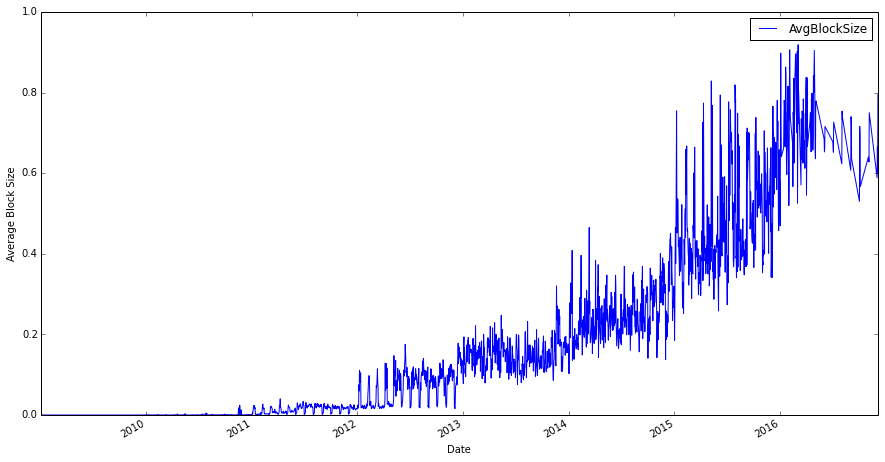
\includegraphics[width=1\linewidth]
    {gfx/avg-block-size-over-time}} 
  \caption{Average Block Size Over Time}
  \label{fig:avg-block-size-over-time}
\end{figure}

In \autoref{fig:avg-block-size-over-time} can be seen how the average
block size has been increasing since the creation of Bitcoin. In 2015
the average block started to dangerously approach the limit of 1 MB,
which is causing a big debate in the Bitcoin community whether they
should increase this limit or not.

\begin{figure}[bth]
  \myfloatalign
  {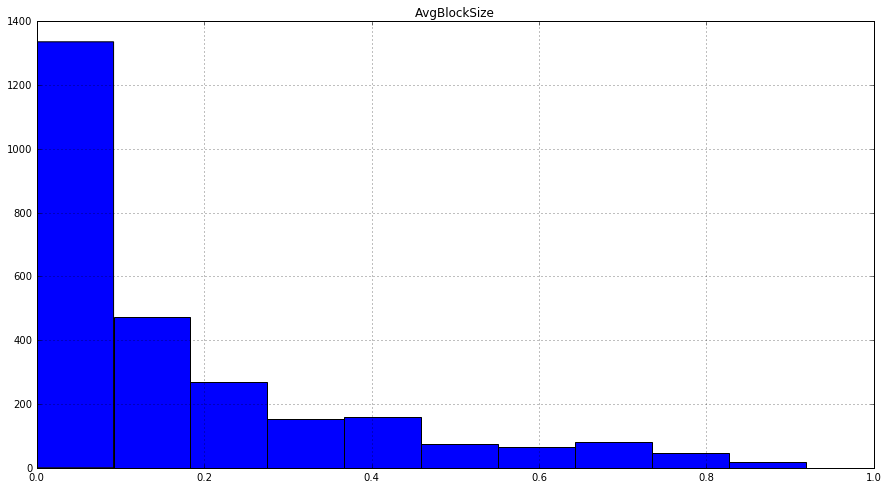
\includegraphics[width=1\linewidth]
    {gfx/avg-block-size-histogram}} 
  \caption{Average Block Size Histogram}
  \label{fig:avg-block-size-histogram}
\end{figure}

\begin{table}
  \myfloatalign
  \small
  \begin{tabularx}{\textwidth}{XX} 
    \toprule
    \tableheadline{Measure} & \tableheadline{Value} \\
    \midrule 
    count  & $2678$\\
    mean   & $0.165078$\\
    median & $0.092355$\\
    std    & $0.209430$\\
    min    & $0.000000$\\
    $25$\% & $0.000899$\\
    $50$\% & $0.092356$\\
    $75$\% & $0.242478$\\
    max    & $0.918519$\\
    \bottomrule
  \end{tabularx}
  \caption{Statistical values for 
    \textit{Average Block Size}}
  \label{tab:stats-avg-block-size}
\end{table}

\begin{figure}[bth]
  \myfloatalign
    {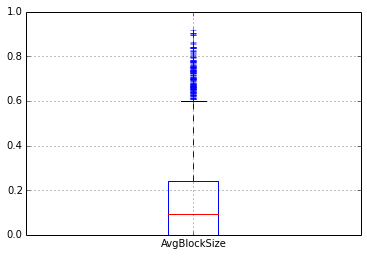
\includegraphics[width=1\linewidth]
      {gfx/avg-block-size-boxplot}}               
    \caption{Average Block Size Boxplot}
    \label{fig:avg-block-size-boxplot}
\end{figure}

\clearpage

%----------------------------------------------------------------------

\subsection{Bitcoin Days Destroyed}
\label{sec:bitcoin-days-destroyed}

\begin{figure}[bth]
  \myfloatalign
  {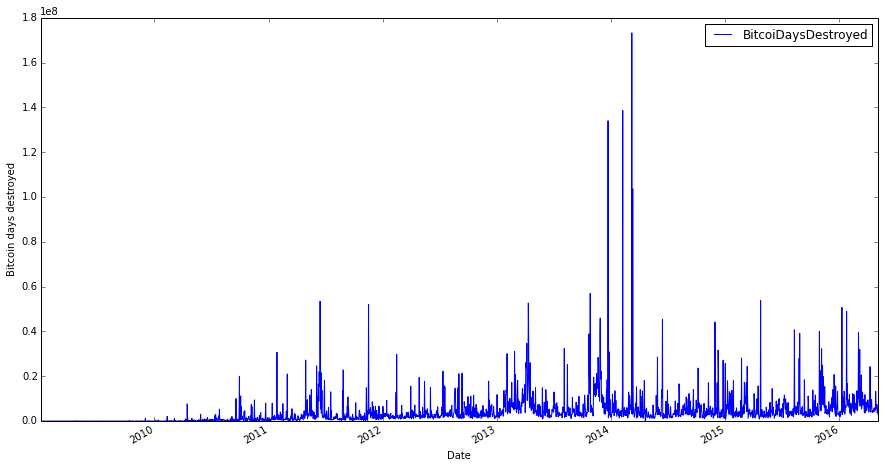
\includegraphics[width=1\linewidth]
    {gfx/bitcoin-days-destroyed-over-time}}
  \caption{Bitcoin Days Destroyed Over Time}
  \label{fig:bitcoin-days-destroyed-over-time}
\end{figure}

Bitcoin Days Destroyed is a weighted measure of aggregate economic
activity, placing value on transacted coins in proportion to the time
they have spent idle on the Bitcoin blockchain. For any given
transaction, Days Destroyed is calculated by multiplying its estimated
transaction value by the number of days since the coins within the
transaction were last spent. Bitcoin Days Destroyed is a useful proxy
for measuring growth in real value transacted on the Bitcoin
blockchain over time, since it controls for rapid movement of coins
between wallets (potentially owned by just one entity). One integer
data point each day, at 18:15:05, spanning from 03/01/2009 to
03/05/2016.

To better understand this variable we include a quote extracted from
\href{http://bitcoin.stackexchange.com/questions/845/what-are-bitcoin-days-destroyed}{Bitcoin
  Beta | Stack Exchange}:

``\textit{The idea of "bitcoin days destroyed" came about because it
  was realized that total transaction volume per day might be an
  inappropriate measure of the level of economic activity in Bitcoin.
  After all, someone could be sending the same money back and forth
  between their own addresses repeatedly. If you sent the same 50 btc
  back and forth 20 times, it would look like 1000 btc worth of
  activity, while in fact it represents almost nothing in terms of
  real transaction volume.}

\textit{With "bitcoin days destroyed", the idea is instead to give
  more weight to coins which haven't been spent in a while. To do
  this, you multiply the amount of each transaction by the number of
  days since those coins were last spent. So, 1 bitcoin that hasn't
  been spent in 100 days (1 bitcoin * 100 days) counts as much as 100
  bitcoins that were just spent yesterday (100 bitcoins * 1 day).
  Because you can think of these "bitcoin days" as building up over
  time until a transaction actually occurs, the actual measure is
  called "bitcoin days destroyed". This is believed to give a better
  indication of how much real economic activity is occurring on the
  bitcoin network.}

\textit{ So how well does it work? Well, it's still not perfect,
  because the other day I moved some coins out of a wallet they've
  been in for several months without spending them or giving them
  away. And some genuine businesses have very rapid turnover in
  bitcoins, so they're not being measured well by this method. But it
  does do a good job of filtering out the "noise" of bitcoins that are
  just "bouncing around" without really going anywhere. The graph of
  overall bitcoin days destroyed is believed to show that the genuine
  level of activity in the Bitcoin economy is continually
  increasing--it's not just one person experimenting by rapidly
  sending the same coins back and forth, flooding the network with
  meaningless chatter. Looks pretty good, hey?}''

\begin{table}
  \myfloatalign
  %\small
  \begin{tabularx}{\textwidth}{XX} 
    \toprule
    \tableheadline{Measure} & \tableheadline{Value} \\
    \midrule 
    count  & $2.679000e+03$ \\
    mean   & $4.146916e+06$ \\
    median & $2456794.0$ \\
    std    & $7.778546e+06$ \\
    min    & $0.000000e+00$ \\
    25\%   & $5.017520e+05$ \\
    50\%   & $2.456794e+06$ \\
    75\%   & $4.745530e+06$ \\
    max    & $1.732980e+08$ \\
    \bottomrule
  \end{tabularx}
  \caption{Statistical values for \textit{Bitcoin Days Destroyed}}
  \label{tab:bitcoin-days-destroyed}
\end{table}

\begin{figure}[bth]
  \myfloatalign
  {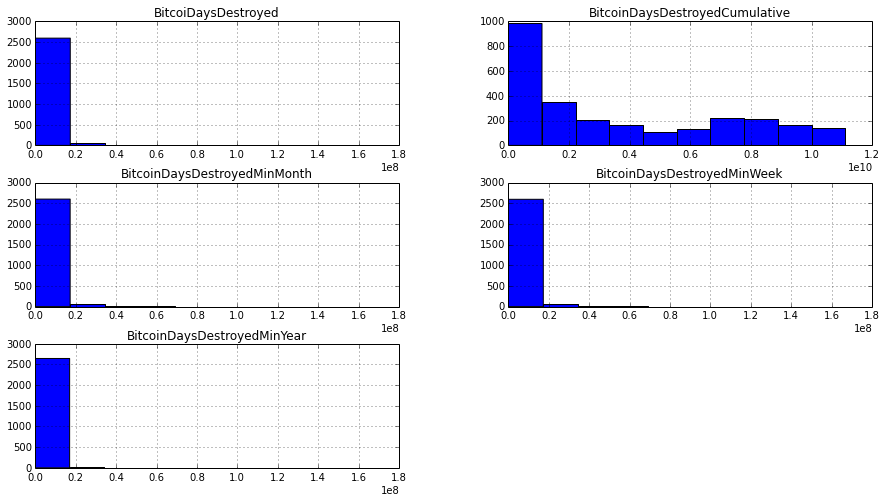
\includegraphics[width=1\linewidth]
    {gfx/bitcoin-days-destroyed-histogram}}
  \caption{Bitcoin Days Destroyed Histogram}
  \label{fig:bitcoin-days-destroyed-histogram}
\end{figure}

\begin{figure}[bth]
  \myfloatalign
  {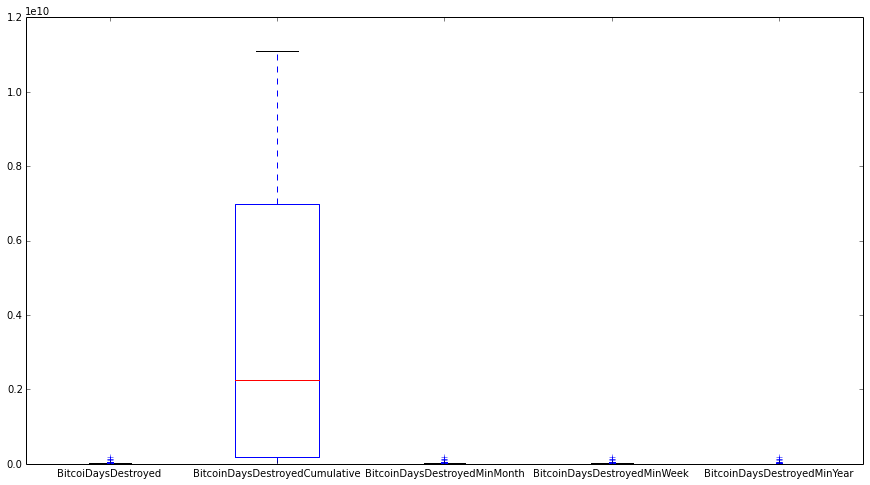
\includegraphics[width=1\linewidth]
    {gfx/bitcoin-days-destroyed-boxplot}}
  \caption{Bitcoin Days Destroyed Boxplot}
  \label{fig:bitcoin-days-destroyed-boxplot}
\end{figure}

\clearpage

%----------------------------------------------------------------------

\subsection{Bitcoin Days Destroyed Min Month}
\label{sec:bitcoin-days-destroyed-min-month}

\begin{figure}[bth]
  \myfloatalign
  {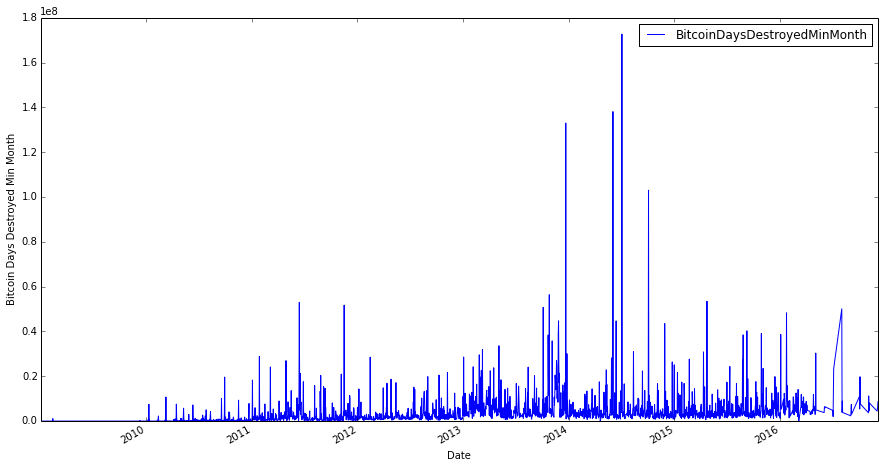
\includegraphics[width=1\linewidth]
    {gfx/bitcoin-days-destroyed-min-month-over-time}}
  \caption{Bitcoin Days Destroyed Min Month Over Time}
  \label{fig:bitcoin-days-destroyed-min-month-over-time}
\end{figure}

Bitcoin Days Destroyed filtered by minimum input age of 1 month. One
integer data point each day at 18:15:05, spanning from 03/01/2009 to
03/05/2016.  

\begin{table}
  \myfloatalign
  %\small
  \begin{tabularx}{\textwidth}{XX} 
    \toprule
    \tableheadline{Measure} & \tableheadline{Value} \\
    \midrule 
    count  & $2.679000e+03$ \\
    mean   & $3.649039e+06$ \\
    median & $1868139$      \\
    std    & $7.629002e+06$ \\
    min    & $0.000000e+00$ \\
    25\%   & $3.028175e+05$ \\
    50\%   & $1.868139e+06$ \\
    75\%   & $4.001042e+06$ \\
    max    & $1.727464e+08$ \\
    \bottomrule
  \end{tabularx}
  \caption{Statistical values for \textit{Bitcoin Days Destroyed Min Month}}
  \label{tab:bitcoin-days-destroyed-min-month}
\end{table}

\begin{figure}[bth]
  \myfloatalign
  {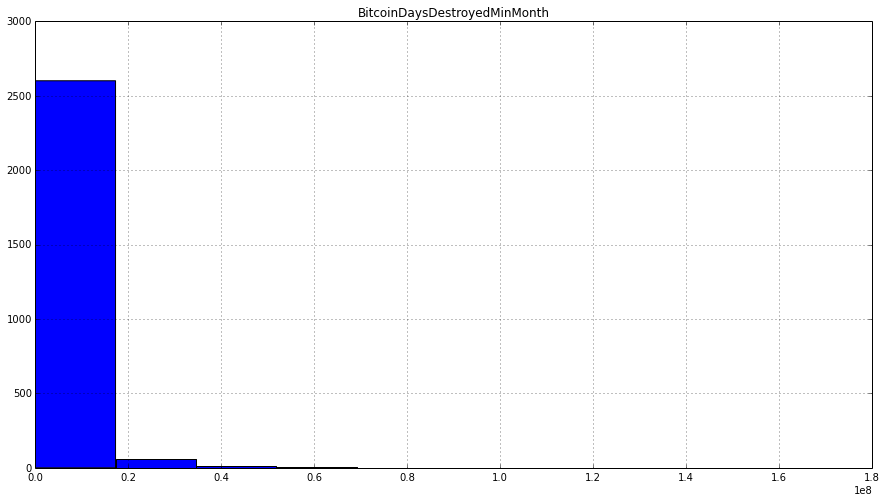
\includegraphics[width=1\linewidth]
    {gfx/bitcoin-days-destroyed-min-month-histogram}}
  \caption{Bitcoin Days Destroyed Min Month Histogram}
  \label{fig:bitcoin-days-destroyed-min-month-histogram}
\end{figure}

\begin{figure}[bth]
  \myfloatalign
  {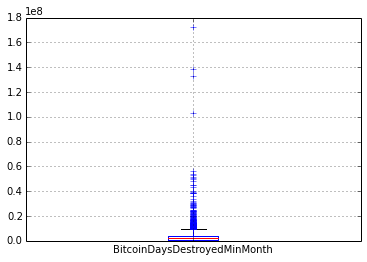
\includegraphics[width=1\linewidth]
    {gfx/bitcoin-days-destroyed-min-month-boxplot}}
  \caption{Bitcoin Days Destroyed Min Month Boxplot}
  \label{fig:bitcoin-days-destroyed-min-month-boxplot}
\end{figure}

\clearpage
%----------------------------------------------------------------------

\subsection{Bitcoin Days Destroyed Min Week}
\label{sec:bitcoin-days-destroyed-min-week}

\begin{figure}[bth]
  \myfloatalign
  {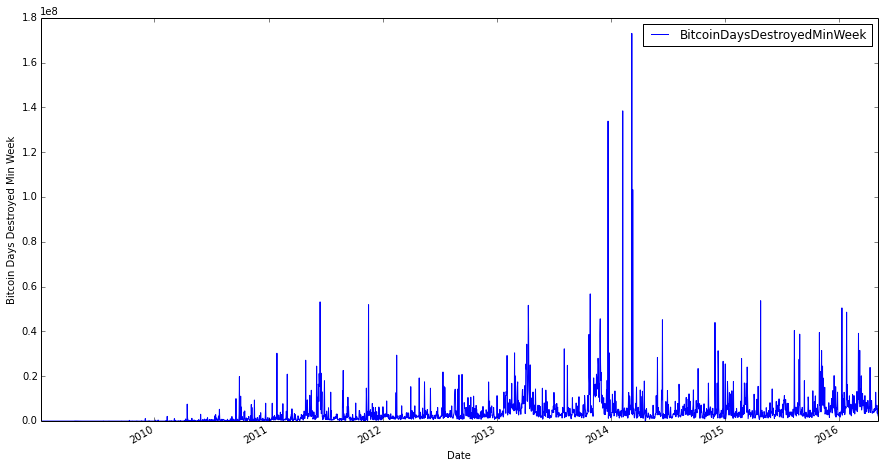
\includegraphics[width=1\linewidth]
    {gfx/bitcoin-days-destroyed-min-week-over-time}}
  \caption{Bitcoin Days Destroyed Min Week Over Time}
  \label{fig:bitcoin-days-destroyed-min-week-over-time}
\end{figure}

Bitcoin Days Destroyed filtered by minimum input age of 1 week. One
integer data point each day at 18:15:05, spanning from 03/01/2009 to
03/05/2016.

\begin{table}
  \myfloatalign
  %\small
  \begin{tabularx}{\textwidth}{XX} 
    \toprule
    \tableheadline{Measure} & \tableheadline{Value} \\
    \midrule 
    count  & $2.679000e+03$ \\
    mean   & $3.947443e+06$ \\
    median & $2210053$      \\
    std    & $7.721971e+06$ \\
    min    & $0.000000e+00$ \\
    25\%   & $4.384805e+05$ \\
    50\%   & $2.210053e+06$ \\
    75\%   & $4.454368e+06$ \\
    max    & $1.730718e+08$ \\
    \bottomrule
  \end{tabularx}
  \caption{Statistical values for \textit{Bitcoin Days Destroyed Min
      Week}} 
  \label{tab:bitcoin-days-destroyed-min-week}
\end{table}

\begin{figure}[bth]
  \myfloatalign
  {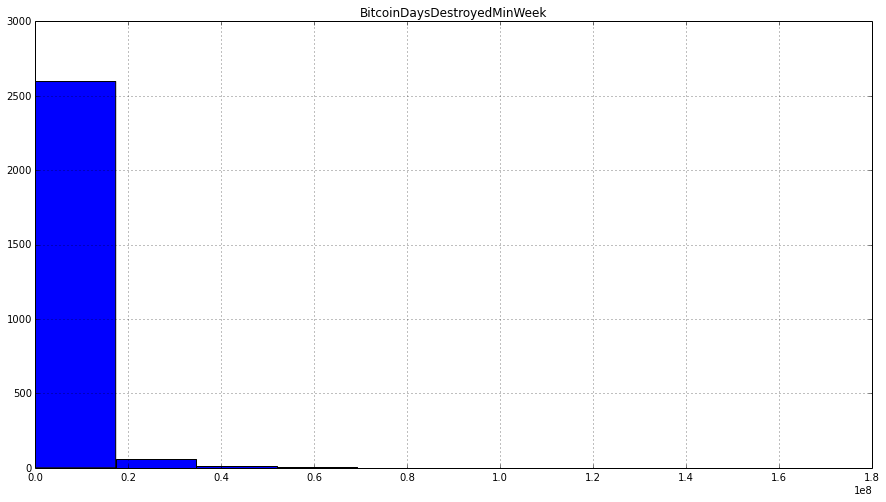
\includegraphics[width=1\linewidth]
    {gfx/bitcoin-days-destroyed-min-week-histogram}}
  \caption{Bitcoin Days Destroyed Min Week Histogram}
  \label{fig:bitcoin-days-destroyed-min-week-histogram}
\end{figure}

\begin{figure}[bth]
  \myfloatalign
  {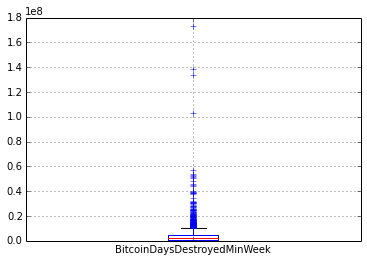
\includegraphics[width=1\linewidth]
    {gfx/bitcoin-days-destroyed-min-week-boxplot}}
  \caption{Bitcoin Days Destroyed Min Week Boxplot}
  \label{fig:bitcoin-days-destroyed-min-week-boxplot}
\end{figure}

\clearpage
%----------------------------------------------------------------------

\subsection{Bitcoin Days Destroyed Min Year}
\label{sec:bitcoin-days-destroyed-min-year}

\begin{figure}[bth]
  \myfloatalign
  {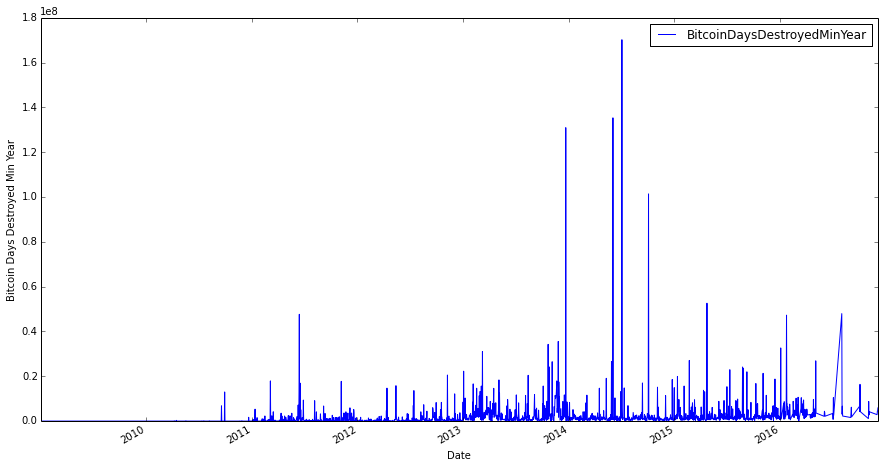
\includegraphics[width=1\linewidth]
    {gfx/bitcoin-days-destroyed-min-year-over-time}}
  \caption{Bitcoin Days Destroyed Min Year Over Time}
  \label{fig:bitcoin-days-destroyed-min-year-over-time}
\end{figure}

Bitcoin Days Destroyed filtered by minimum input age of 1 year. One
integer data point each day at 18:15:05, spanning from 03/01/2009 to
03/05/2016.

\begin{table}
  \myfloatalign
  %\small
  \begin{tabularx}{\textwidth}{XX} 
    \toprule
    \tableheadline{Measure} & \tableheadline{Value} \\
    \midrule 
    count  & $2.679000e+03$ \\
    mean   & $1.774081e+06$ \\
    median & $416483.0$     \\
    std    & $6.404385e+06$ \\
    min    & $0.000000e+00$ \\
    25\%   & $0.000000e+00$ \\
    50\%   & $4.164830e+05$ \\
    75\%   & $1.568172e+06$ \\
    max    & $1.702367e+08$ \\
    \bottomrule
  \end{tabularx}
  \caption{Statistical values for \textit{Bitcoin Days Destroyed Min
      Year}} 
  \label{tab:bitcoin-days-destroyed-min-year}
\end{table}

\begin{figure}[bth]
  \myfloatalign
  {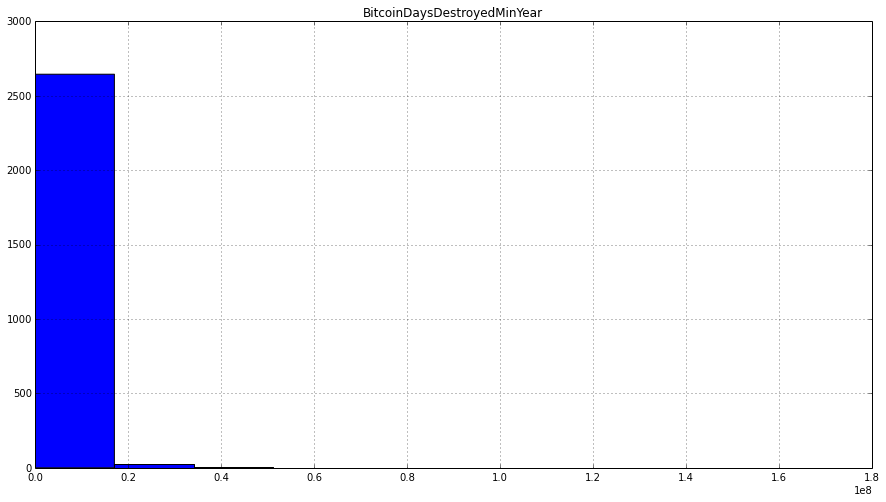
\includegraphics[width=1\linewidth]
    {gfx/bitcoin-days-destroyed-min-year-histogram}}
  \caption{Bitcoin Days Destroyed Min Year Histogram}
  \label{fig:bitcoin-days-destroyed-min-year-histogram}
\end{figure}

\begin{figure}[bth]
  \myfloatalign
  {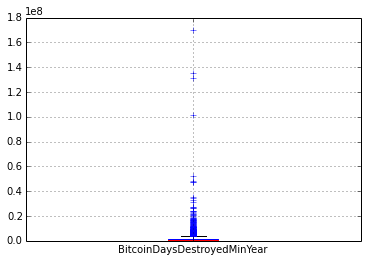
\includegraphics[width=1\linewidth]
    {gfx/bitcoin-days-destroyed-min-year-boxplot}}
  \caption{Bitcoin Days Destroyed Min Year Boxplot}
  \label{fig:bitcoin-days-destroyed-min-year-boxplot}
\end{figure}

\clearpage
%----------------------------------------------------------------------

\subsection{Bitcoin Days Destroyed Cumulative}
\label{sec:bitcoin-days-destroyed-cumulative}

\begin{figure}[bth]
  \myfloatalign
  {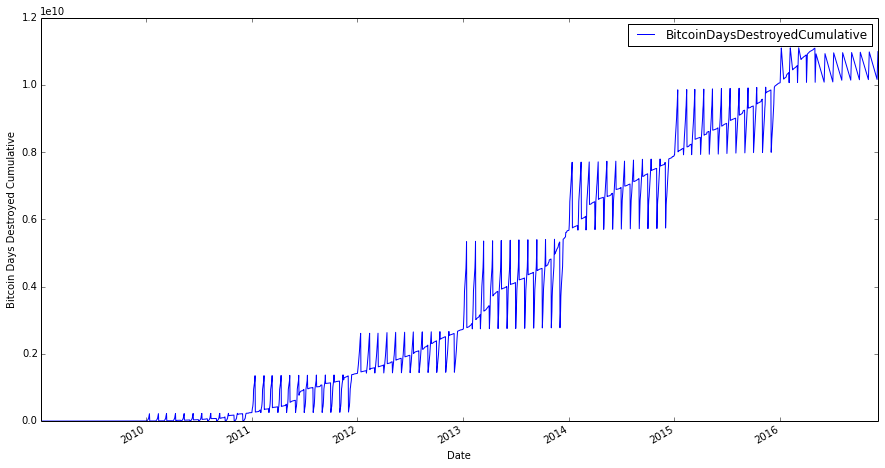
\includegraphics[width=1\linewidth]
    {gfx/bitcoin-days-destroyed-cumulative-over-time}}
  \caption{Bitcoin Days Destroyed Cumulative Over Time}
  \label{fig:bitcoin-days-destroyed-cumulative-over-time}
\end{figure}

Bitcoin Days Destroyed Cumulative acumulates all the bitcoins days
destroyed. That means that the increase of these variable shows the
increase in ``real'' transactions. In
\autoref{fig:bitcoin-days-destroyed-cumulative-over-time} we can see
that the value of this variable keeps growing, which leads us to think
that the ``real'' use of Bitcoin is also growin.

All the ``Bitcoin Days Destroyed'' variables are useful to disciminate
the ``real'' transaction between people and the rapid transaction
that can be done by traders for example.

The dataset comprises one integer data point each day, at
18:15:05, spanning from 03/01/2009 to 03/05/2016.

\begin{table}
  \myfloatalign
  %\small
  \begin{tabularx}{\textwidth}{XX} 
    \toprule
    \tableheadline{Measure} & \tableheadline{Value} \\
    \midrule 
    count  & $2.679000e+03$ \\
    mean   & $3.609471e+09$ \\
    median & $2265772771.0$ \\
    std    & $3.572547e+09$ \\
    min    & $0.000000e+00$ \\
    25\%   & $1.817693e+08$ \\
    50\%   & $2.265773e+09$ \\
    75\%   & $6.971917e+09$ \\
    max    & $1.110959e+10$ \\ 
    \bottomrule
  \end{tabularx}
  \caption{Statistical values for \textit{Bitcoin Days Destroyed Cumulative}}
  \label{tab:bitcoin-days-destroyed-cumulative}
\end{table}

\begin{figure}[bth]
  \myfloatalign
  {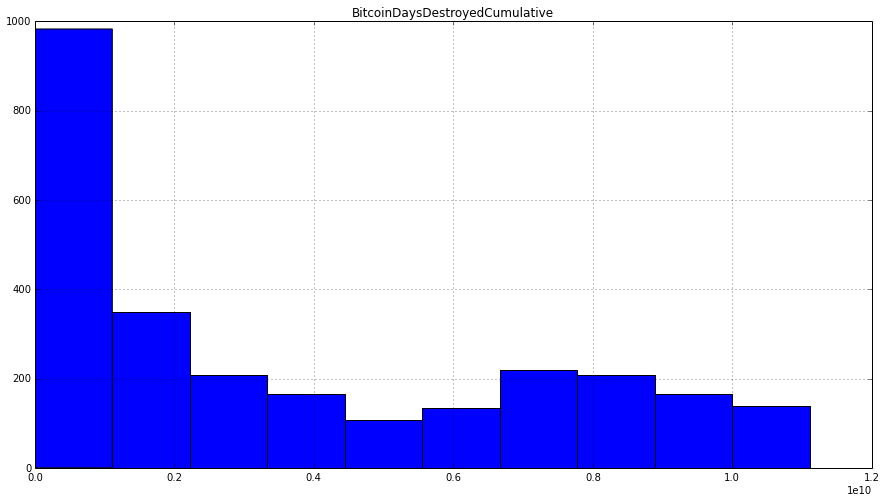
\includegraphics[width=1\linewidth]
    {gfx/bitcoin-days-destroyed-cumulative-histogram}}
  \caption{Bitcoin Days Destroyed Cumulative Histogram}
  \label{fig:bitcoin-days-destroyed-cumulative-histogram}
\end{figure}

\begin{figure}[bth]
  \myfloatalign
  {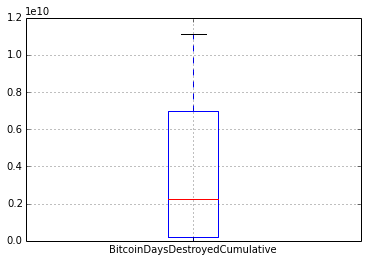
\includegraphics[width=1\linewidth]
    {gfx/bitcoin-days-destroyed-cumulative-boxplot}}
  \caption{Bitcoin Days Destroyed Cumulative Boxplot}
  \label{fig:bitcoin-days-destroyed-cumulative-boxplot}
\end{figure}

\clearpage
%----------------------------------------------------------------------

\subsection{Block Size}
\label{sec:block-size}

\begin{figure}[bth]
  \myfloatalign
  {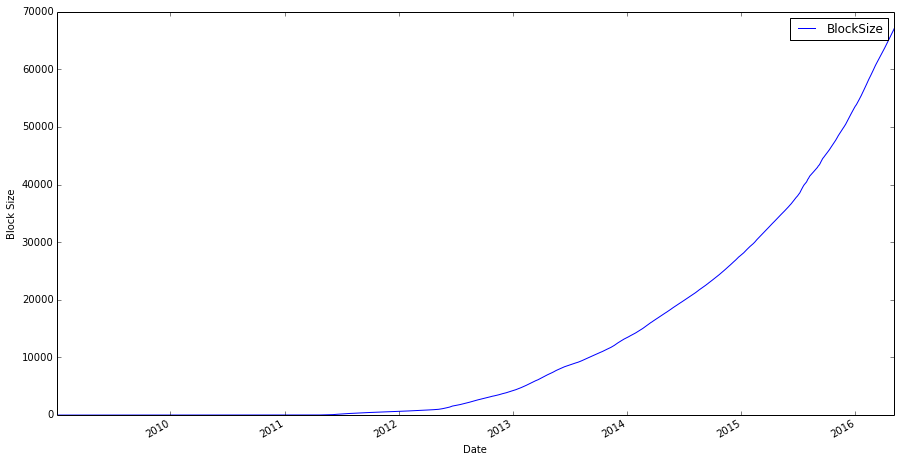
\includegraphics[width=1\linewidth]
    {gfx/block-size-over-time}}
  \caption{Block Size Over Time}
  \label{fig:block-size-over-time}
\end{figure}

The total size (in MB) of all block headers and transactions. Not
including database indexes. One real number data point each day, at
18:15:05, spanning from 03/01/2009 to 03/05/2016.

The total block size is increasing exponentialy as seen in
\autoref{fig:block-size-over-time}. This basically represents that the
total ammount of transactions are increasing at that rate.

\begin{table}
  \myfloatalign
  %\small
  \begin{tabularx}{\textwidth}{XX} 
    \toprule
    \tableheadline{Measure} & \tableheadline{Value} \\
    \midrule 
    count  & $2678.000000$       \\
    mean   & $9.727391$          \\
    median & $6.219650292785771$ \\
    std    & $13.268846$         \\
    min    & $0.000000$          \\
    25\%   & $1.301186$          \\
    50\%   & $6.219650$          \\
    75\%   & $10.401306$         \\
    max    & $90.202095$         \\
    \bottomrule
  \end{tabularx}
  \caption{Statistical values for \textit{Block Size}}
  \label{tab:block-size}
\end{table}

\begin{figure}[bth]
  \myfloatalign
  {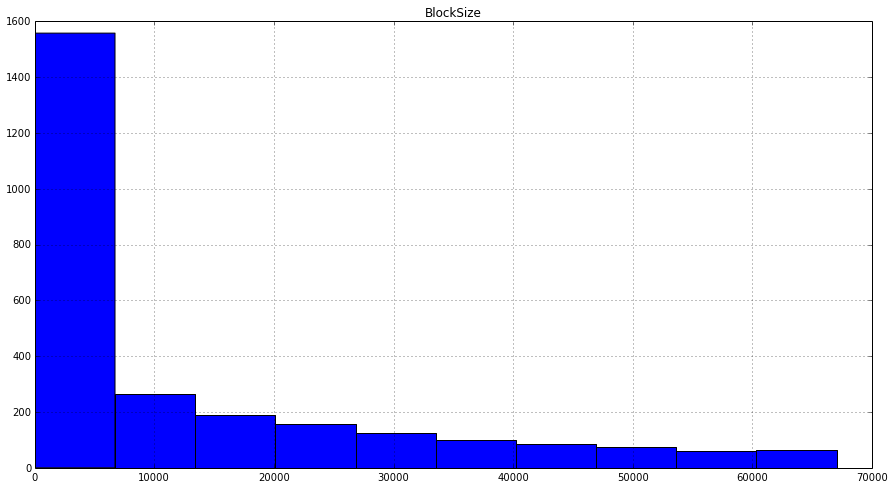
\includegraphics[width=1\linewidth]
    {gfx/block-size-histogram}}
  \caption{Block Size Histogram}
  \label{fig:block-size-histogram}
\end{figure}

\begin{figure}[bth]
  \myfloatalign
  {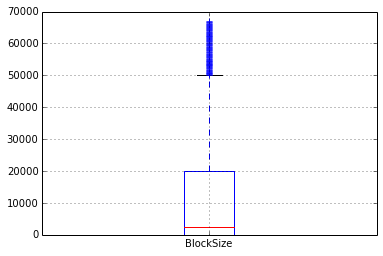
\includegraphics[width=1\linewidth]
    {gfx/block-size-boxplot}}
  \caption{Block Size Boxplot}
  \label{fig:block-size-boxplot}
\end{figure}

\clearpage
%----------------------------------------------------------------------

\subsection{Cost Per Transaction}
\label{sec:cost-per-transaction}

This variable shows miners revenue (in USD) divided by the number of
transactions. To better understand the fluctuations of \textit{Cost
  Per Transaction} show in
\autoref{fig:cost-per-transaction-over-time} we include the next
definition, found
\href{https://en.bitcoin.it/wiki/Transaction_fees}{here}:

\textit{``The transaction fee is processed by and received by the
  bitcoin miner. When a new bitcoin block is generated with a
  successful hash, the information for all of the transactions is
  included with the block and all transaction fees are collected by
  that user creating the block, who is free to assign those fees to
  himself.}

\textit{Transaction fees are voluntary on the part of the person
  making the bitcoin transaction, as the person attempting to make a
  transaction can include any fee or none at all in the transaction.
  On the other hand, nobody mining new bitcoins necessarily needs to
  accept the transactions and include them in the new block being
  created. The transaction fee is therefore an incentive on the part
  of the bitcoin user to make sure that a particular transaction will
  get included into the next block which is generated.''}

Knowing how the fees work in Bitcoin, we can see that the cost depends
on the will of the miner to accept or not the transaction. If we look
at \autoref{fig:n-transactions-over-time} we can see that there is
some correlation between the number of transactions been processed and
the cost of each transaction. The first peek in both figures coincide
around January/2011, after that, in mid 2011 there is a sustained
increase in the number of transactions, which in
\autoref{fig:cost-per-transaction-over-time} has a counterpart peek in
the cost of transactions, probably, because a lot of people wanted to
make transactions and the amount of miners were small. After that the
cost per transaction lowers and doesn't have a significant increase
till mid 2013. This increase is due to an increase in trade volume,
that can be seen clearly in \autoref{fig:trade-volume-over-time}. Next
to that, we see the biggest cost of cost per transaction so far, which
took place in the end of 2013 and start of 2014. This peek also occurs
simultaneously to a trade volume peek.

\begin{figure}[bth]
  \myfloatalign
  {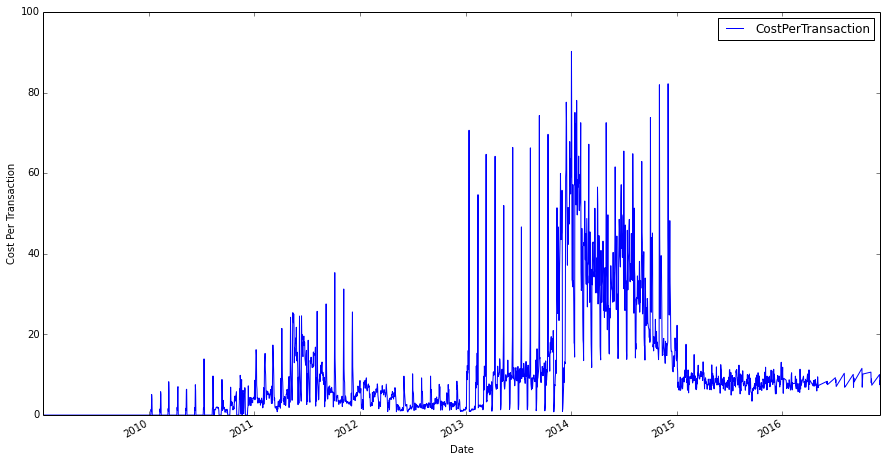
\includegraphics[width=1\linewidth]
    {gfx/cost-per-transaction-over-time}}
  \caption{Cost Per Transaction Over Time}
  \label{fig:cost-per-transaction-over-time}
\end{figure}

The dataset comprises one real number data point each day, at
18:15:05, spanning from 03/01/2009 to 03/05/2016.

\begin{table}
  \myfloatalign
  %\small
  \begin{tabularx}{\textwidth}{XX} 
    \toprule
    \tableheadline{Measure} & \tableheadline{Value} \\
    \midrule 
    count  & $2678$ \\
    mean   & $9.727391$    \\
    median & $6.21965$     \\
    std    & $13.268846$   \\
    min    & $0$    \\
    $25$\  & $1.301186$    \\
    $50$\  & $6.219650$    \\
    $75$\  & $10.401306$   \\
    max    & $90.202095$   \\
    \bottomrule
  \end{tabularx}
  \caption{Statistical values for \textit{Cost Per Transaction}}
  \label{tab:cost-per-transaction}
\end{table}

\begin{figure}[bth]
  \myfloatalign
  {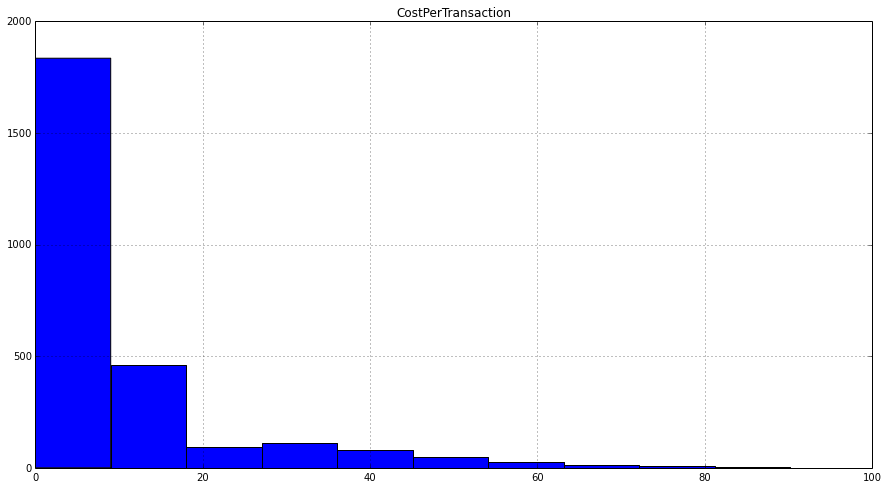
\includegraphics[width=1\linewidth]
    {gfx/cost-per-transaction-histogram}}
  \caption{Cost Per Transaction Histogram}
  \label{fig:cost-per-transaction-histogram}
\end{figure}

\begin{figure}[bth]
  \myfloatalign
  {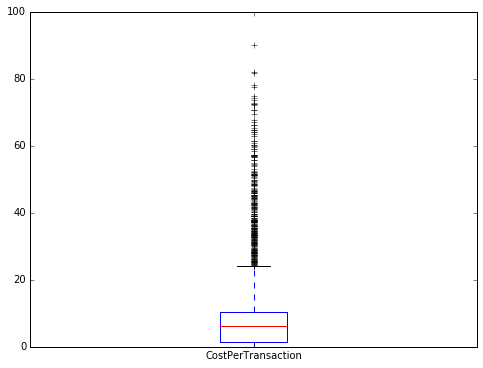
\includegraphics[width=1\linewidth]
    {gfx/cost-per-transaction-boxplot}}
  \caption{Cost Per Transaction Boxplot}
  \label{fig:cost-per-transaction-boxplot}
\end{figure}

\clearpage
%----------------------------------------------------------------------

\subsection{Cost Per Transaction Percent}
\label{sec:cost-per-transaction-percent}

\begin{figure}[bth]
  \myfloatalign
  {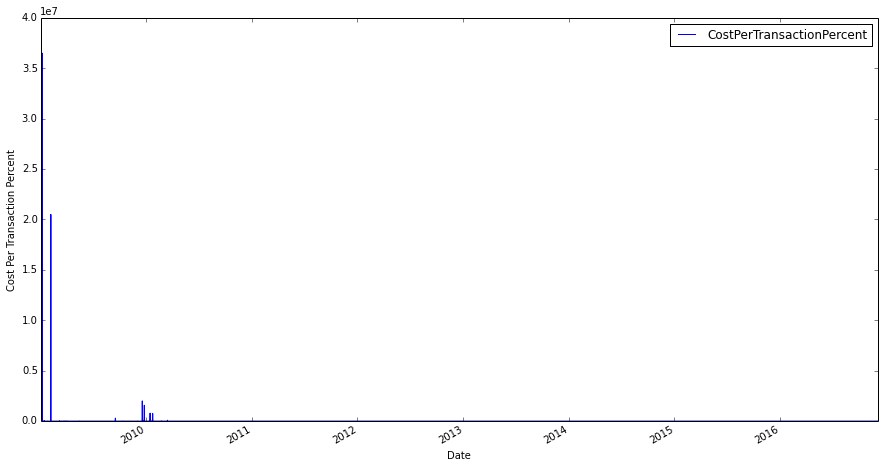
\includegraphics[width=1\linewidth]
    {gfx/cost-per-transaction-percent-over-time}}
  \caption{Cost Per Transaction Percent Over Time}
  \label{fig:cost-per-transaction-percent-over-time}
\end{figure}

This variable shows miners revenue as percentage of the transaction
volume. Basically what
\autoref{fig:cost-per-transaction-percent-over-time} shows is that
over time, the transactions fees are decreasing with respect to the
transaction amount itself. The median, shown in
\autoref{tab:cost-per-transaction-percent}, is $3.283375136886966\%$,
which reflects the percent of transaction that is used mostly in all
Bitcoin transactions.

The dataset comprises one real number data point each day, at
18:15:05, spanning from 03/01/2009 to 03/05/2016.

\begin{table}
  \myfloatalign
  %\small
  \begin{tabularx}{\textwidth}{XX} 
    \toprule
    \tableheadline{Measure} & \tableheadline{Value} \\
    \midrule 
    count  & $2678.000000$       \\
    mean   & $23603.541449$      \\
    median & $3.283375136886966$ \\
    std    & $810554.930805$     \\
    min    & $0.000000$          \\
    25\%   & $1.580112$          \\
    50\%   & $3.283375$          \\
    75\%   & $9.606991$          \\
    max    & $36500000.000000$   \\
    \bottomrule
  \end{tabularx}
  \caption{Statistical values for \textit{Cost Per Transaction Percent}}
  \label{tab:cost-per-transaction-percent}
\end{table}

\begin{figure}[bth]
  \myfloatalign
  {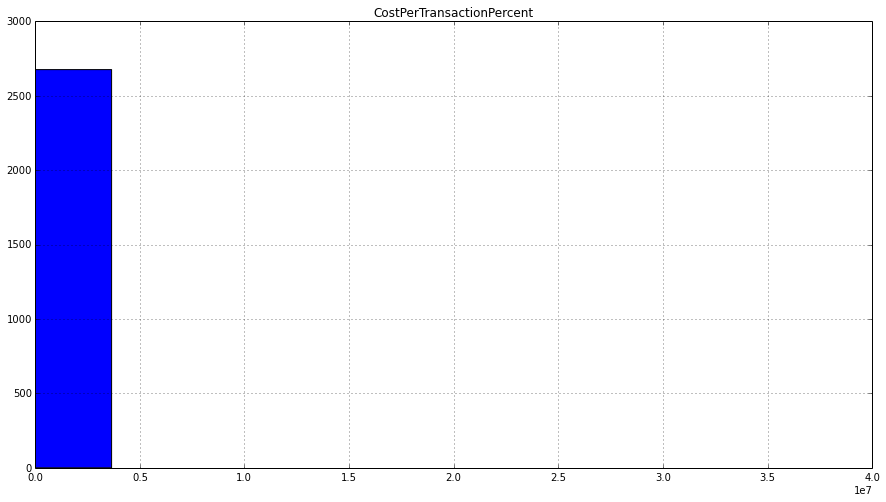
\includegraphics[width=1\linewidth]
    {gfx/cost-per-transaction-percent-histogram}}
  \caption{Cost Per Transaction Percent Histogram}
  \label{fig:cost-per-transaction-percent-histogram}
\end{figure}

\begin{figure}[bth]
  \myfloatalign
  {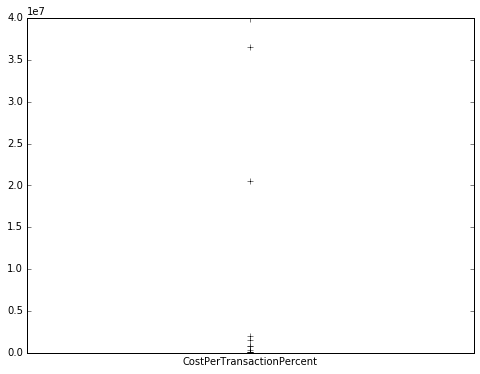
\includegraphics[width=1\linewidth]
    {gfx/cost-per-transaction-percent-boxplot}}
  \caption{Cost Per Transaction Percent Boxplot}
  \label{fig:cost-per-transaction-percent-boxplot}
\end{figure}

\clearpage
%----------------------------------------------------------------------

\subsection{Difficulty}
\label{sec:difficulty}

\begin{figure}[bth]
  \myfloatalign
  {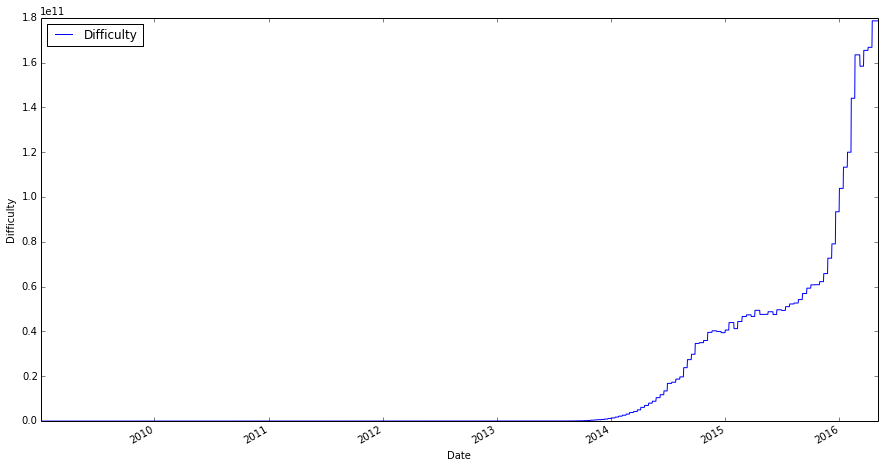
\includegraphics[width=1\linewidth]
    {gfx/difficulty-over-time}}
  \caption{Difficulty Over Time}
  \label{fig:difficulty-over-time}
\end{figure}

A relative measure of how difficult it is to find a new block. The
difficulty is adjusted periodically as a function of how much hashing
power has been deployed by the network of miners. That can be seen
looking at how similar are \autoref{fig:difficulty-over-time} and
\autoref{fig:hash-rate-over-time}. The graphic representing the
difficulty has a discrete shape, that is because the difficulty is
adjusted automatically every 2016 blocks, and changes equally for the
entire Bitcoin network. Until 2014, the difficulty of mining was
very low, it started to raise probably because the trade volume in the
end of 2013 and start of 2014 was approximately 70.000.000\$, which
attracted professional miners with a greater processing power, those
creating more and more blocks and augmenting the difficulty of mining.

The dataset comprises one real number data point each day, at
18:15:05, spanning from 03/01/2009 to 03/05/2016.

\begin{table}
  \myfloatalign
  %\small
  \begin{tabularx}{\textwidth}{XX} 
    \toprule
    \tableheadline{Measure} & \tableheadline{Value} \\
    \midrule 
    count  & $2.678000e+03$      \\
    mean   & $1.683580e+10$      \\
    median & $2440642.606915964$ \\
    std    & $3.561708e+10$      \\
    min    & $0.000000e+00$      \\
    25\%   & $3.091737e+03$      \\
    50\%   & $2.440643e+06$      \\
    75\%   & $1.681846e+10$      \\
    max    & $1.786783e+11$      \\
    \bottomrule
  \end{tabularx}
  \caption{Statistical values for \textit{Difficulty}}
  \label{tab:difficulty}
\end{table}

\begin{figure}[bth]
  \myfloatalign
  {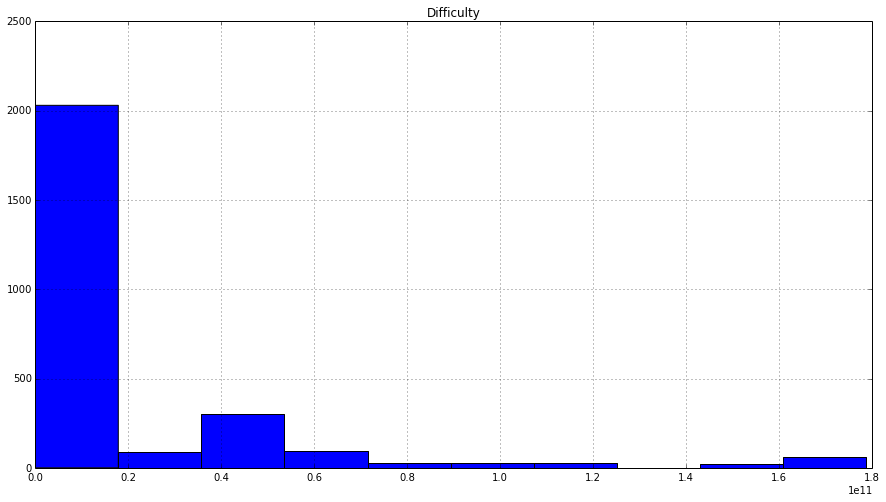
\includegraphics[width=1\linewidth]
    {gfx/difficulty-histogram}}
  \caption{Difficulty Histogram}
  \label{fig:difficulty-histogram}
\end{figure}

\begin{figure}[bth]
  \myfloatalign
  {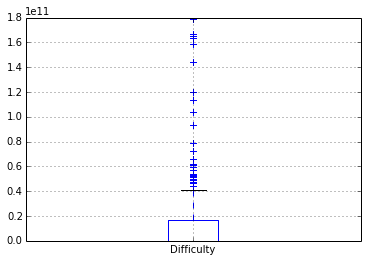
\includegraphics[width=1\linewidth]
    {gfx/difficulty-boxplot}}
  \caption{Difficulty Boxplot}
  \label{fig:difficulty-boxplot}
\end{figure}

\clearpage
%----------------------------------------------------------------------

\subsection{Estimated Transaction Volume}
\label{sec:estimated-transaction-volume}

\begin{figure}[bth]
  \myfloatalign
  {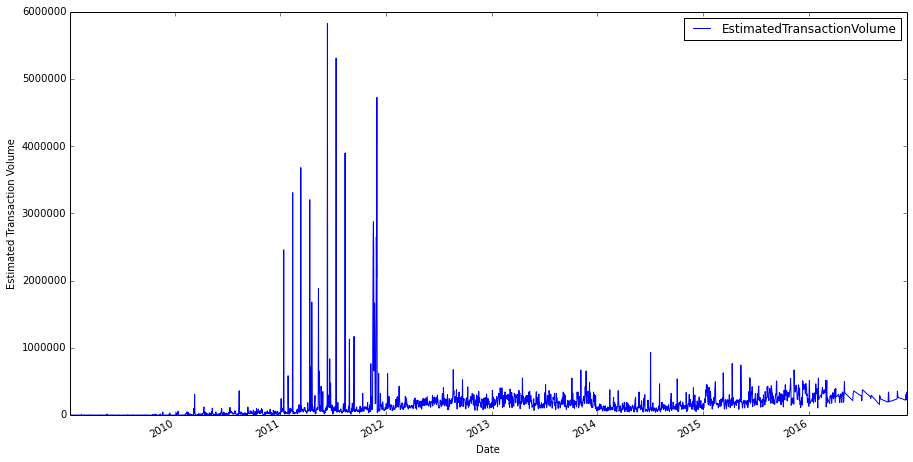
\includegraphics[width=1\linewidth]
    {gfx/estimated-transaction-volume-over-time}}
  \caption{Estimated Transaction Volume Over Time}
  \label{fig:estimated-transaction-volume-over-time}
\end{figure}

The total estimated value of transactions on the Bitcoin blockchain
(does not include coins returned to sender as change). The transaction
volume represented in
\autoref{fig:estimated-transaction-volume-over-time} is very slowly
increasing, meaning that more transactions in Bitcoin are processed.
However, it doesn't represent the actual value of transactions,
because people think in their local currency when trading or shopping,
and Bitcoin's value is volatile. Is more useful the next variable,
\textit{Estimated Transaction Volume USD} that gives as tells the
actual value of transactions. The peak that happened in 2012 wouldn't
occur easily today due to the current value of Bitcoin.

The data-set comprises one integer data point each day, at
18:15:05, spanning from 03/01/2009 to 03/05/2016.

\begin{table}
  \myfloatalign
  %\small
  \begin{tabularx}{\textwidth}{XX} 
    \toprule
    \tableheadline{Measure} & \tableheadline{Value} \\
    \midrule 
    count  & $2679.000000$    \\
    mean   & $157340.920119$  \\
    median & $118843.0$       \\
    std    & $282285.024788$  \\
    min    & $0.000000$       \\
    $25$\% & $30553.000000$   \\
    $50$\% & $118843.000000$  \\
    $75$\% & $210442.000000$  \\
    max    & $5825066.000000$ \\
    \bottomrule
  \end{tabularx}
  \caption{Statistical values for \textit{Estimated Transaction Volume}}
  \label{tab:estimated-transaction-volume}
\end{table}

\begin{figure}[bth]
  \myfloatalign
  {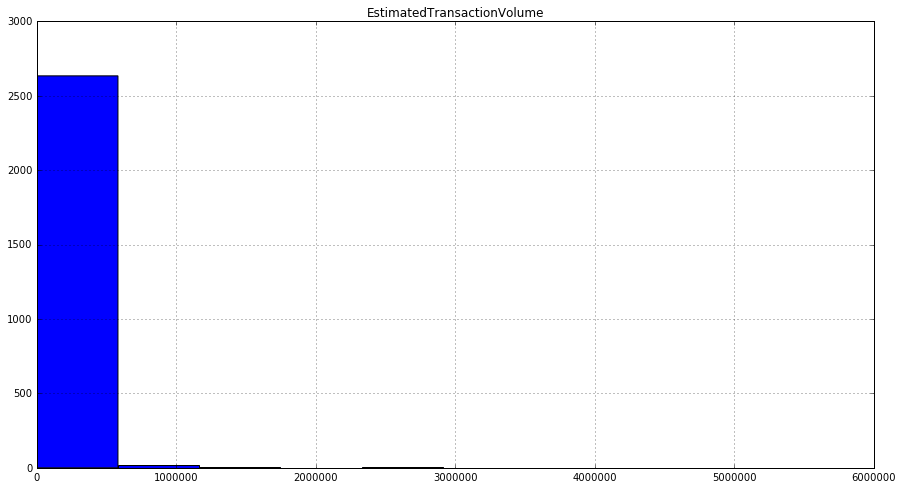
\includegraphics[width=1\linewidth]
    {gfx/estimated-transaction-volume-histogram}}
  \caption{Estimated Transaction Volume Histogram}
  \label{fig:estimated-transaction-volume-histogram}
\end{figure}

\begin{figure}[bth]
  \myfloatalign
  {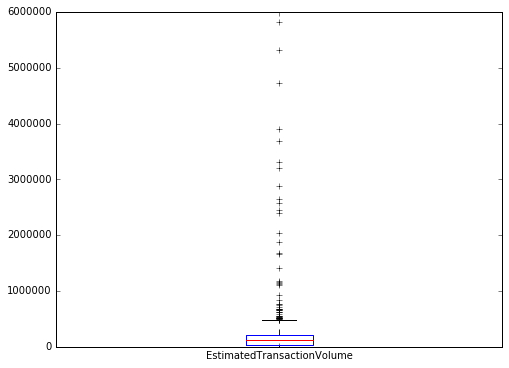
\includegraphics[width=1\linewidth]
    {gfx/estimated-transaction-volume-boxplot}}
  \caption{Estimated Transaction Volume Boxplot}
  \label{fig:estimated-transaction-volume-boxplot}
\end{figure}

\clearpage
%----------------------------------------------------------------------

\subsection{Estimated Transaction Volume USD}
\label{sec:estimated-transaction-volume-usd}

\begin{figure}[bth]
  \myfloatalign
  {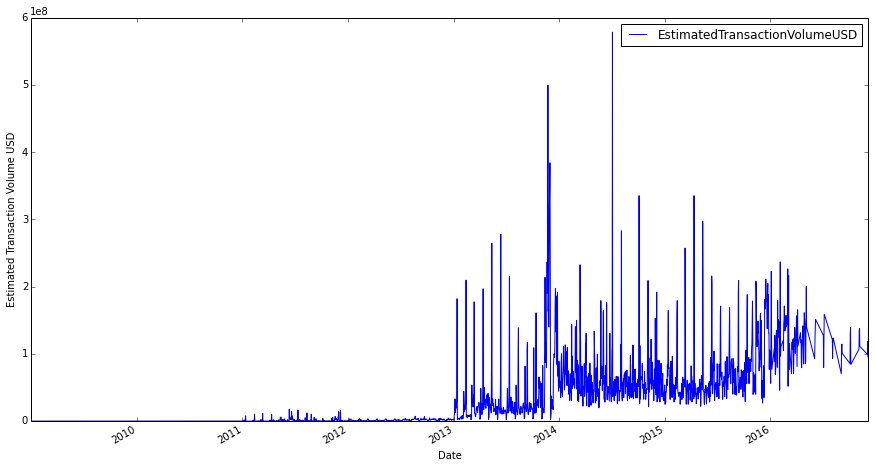
\includegraphics[width=1\linewidth]
    {gfx/estimated-transaction-volume-usd-over-time}}
  \caption{Estimated Transaction Volume USD Over Time}
  \label{fig:estimated-transaction-volume-usd-over-time}
\end{figure}

The Estimated Transaction Volume in USD value, shown in
\autoref{fig:estimated-transaction-volume-usd-over-time}, can be
explained by the average value of Bitcoin, shown in
\autoref{fig:market-price-over-time}, because nearly all the events
are paired in the two figures. There is a small increase in estimated
transaction volume in USD in mid 2011 at the same time than the
average price of Bitcoin increases. Later on, in 2013 there is a
bigger increase in estimated volume that is also reflected in the
average price. Then we have the two biggest peaks around January of
2014 coinciding with the higher average value of Bitcoin (also
represented in two peaks). After that there is decrease in average
price and estimated volume till 2016 where Bitcoin average price
starts to increase at the same time that the estimate transaction
volume increases.

This data-set comprises one integer data point each day, at 18:15:05,
spanning from 03/01/2009 to 03/05/2016.

\begin{table}
  \myfloatalign
  %\small
  \begin{tabularx}{\textwidth}{XX} 
    \toprule
    \tableheadline{Measure} & \tableheadline{Value} \\
    \midrule 
    count  & $2.679000e+03$ \\
    median & $2481424.0$    \\
    mean   & $3.018470e+07$ \\
    std    & $4.923048e+07$ \\
    min    & $0.000000e+00$ \\
    $25$\% & $5.086000e+03$ \\
    $50$\% & $2.481424e+06$ \\
    $75$\% & $4.761785e+07$ \\
    max    & $5.787707e+08$ \\
    \bottomrule
  \end{tabularx}
  \caption{Statistical values for \textit{Estimated Transaction Volume USD}}
  \label{tab:estimated-transaction-volume-usd}
\end{table}

\begin{figure}[bth]
  \myfloatalign
  {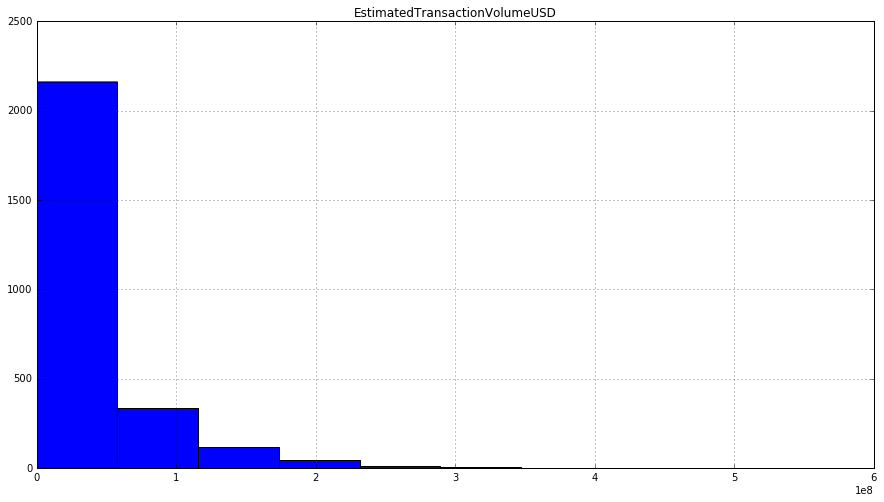
\includegraphics[width=1\linewidth]
    {gfx/estimated-transaction-volume-usd-histogram}}
  \caption{Estimated Transaction Volume USD Histogram}
  \label{fig:estimated-transaction-volume-usd-histogram}
\end{figure}

\begin{figure}[bth]
  \myfloatalign
  {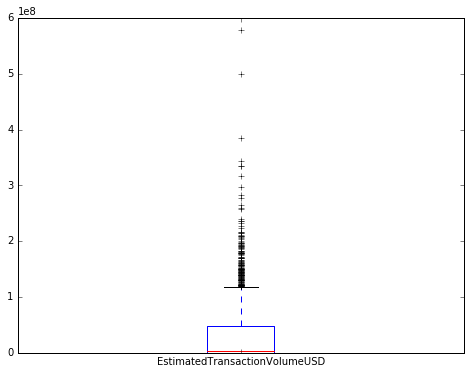
\includegraphics[width=1\linewidth]
    {gfx/estimated-transaction-volume-usd-boxplot}}
  \caption{Estimated Transaction Volume USD Boxplot}
  \label{fig:estimated-transaction-volume-usd-boxplot}
\end{figure}

\clearpage

%----------------------------------------------------------------------

\subsection{Euro price in USD}
\label{sec:euro-price-in-usd}

\begin{figure}[bth]
  \myfloatalign
  {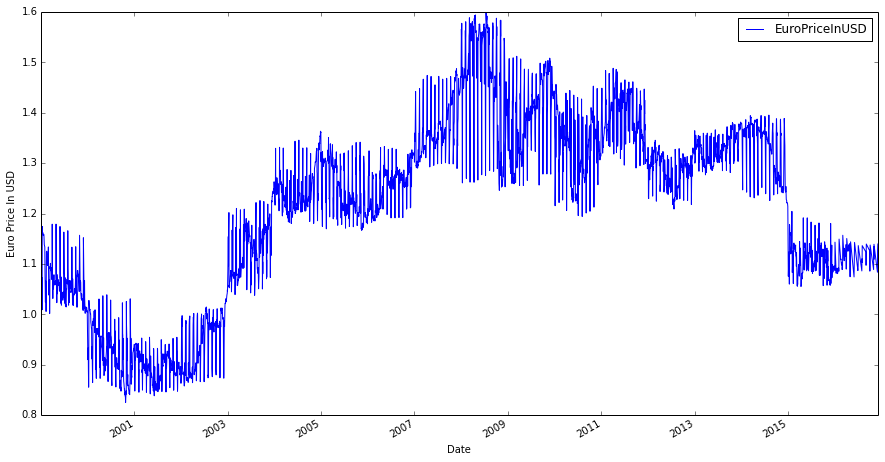
\includegraphics[width=1\linewidth]
    {gfx/euro-price-in-usd-over-time}} 
  \caption{Euro price in USD Over Time}
  \label{fig:euro-price-in-usd-over-time}
\end{figure}

Euro price in USD provided by the European Central Bank from the
creation of the Euro. One real data entry per day, spanning from
04/01/1999 to 10/05/2016.

This dataset has latent values. We have used interpolation in order to
fill the missing values.

As shown in \autoref{fig:euro-price-in-usd-over-time} the value of Euro
has been above that of the USD from its creation, been the period of
2000 through 2003 its closer price to each other. From 2003 to 2007
the price of the Euro increased, coinciding with an increase on the
interest imposed by the BCE. This increase in the interest of the
credits is followed by the collapse of the housing bubble in 2007,
where the price of the Euro kept increasing, altough the interest was
maintained by the BCE until 2009 where the BCE started to lower it.
The increase in the Euro price is probably due to strategies of the
Federal Reserve to lower the price of the USD. Finally in 2015, the
BCE lowered the interests of credits approaching the $0.0\%$, and
that's reflected with a decrease in the price of the Euro with respect
to USD.

\begin{table}
  \myfloatalign
  %\small
  \begin{tabularx}{\textwidth}{XX} 
    \toprule
    \tableheadline{Measure} & \tableheadline{Value} \\
    \midrule 
    count & 4443\\
    mean  & 1.216306\\
    median & 1.2579\\
    std   & 0.177679\\
    min   & 0.825200\\
    25\%  & 1.088300\\
    50\%  & 1.257900\\
    75\%  & 1.345050\\
    max   & 1.599000\\
    \bottomrule
  \end{tabularx}
  \caption{Statistical values for \textit{Euro price in USD}}
  \label{tab:euro-price-in-usd}
\end{table}

There are 62 missing values in the data which has been interpolated
after obtaining the descriptive variables of
\autoref{tab:euro-price-in-usd}

\begin{figure}[bth]
  \myfloatalign
  {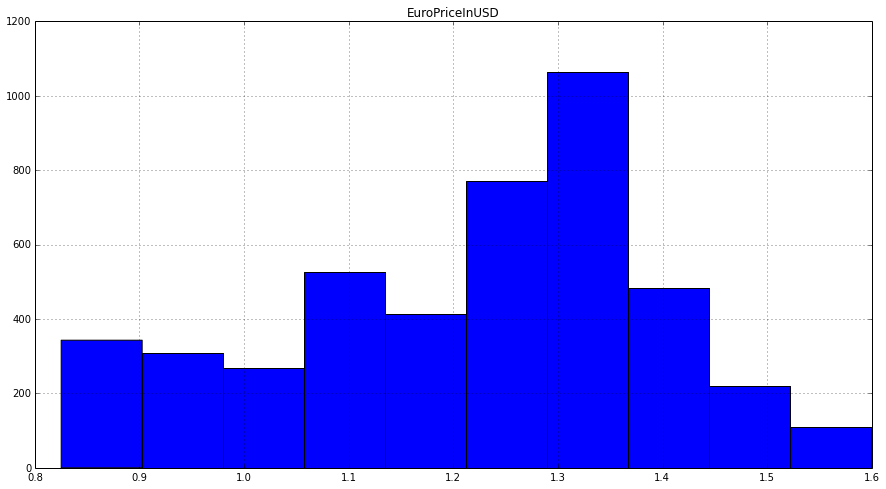
\includegraphics[width=1\linewidth]
    {gfx/euro-price-in-usd-histogram}} 
  \caption{Euro price in USD Histogram}
  \label{fig:euro-price-in-usd-histogram}
\end{figure}

\begin{figure}[bth]
  \myfloatalign
  {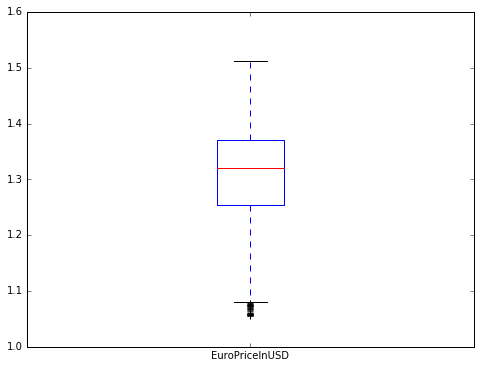
\includegraphics[width=1\linewidth]
    {gfx/euro-price-in-usd-boxplot}}
  \caption{Euro price in USD Boxplot}
  \label{fig:euro-price-in-usd-boxplot}
\end{figure}

\clearpage

%----------------------------------------------------------------------

\subsection{Hash Rate}
\label{sec:hash-rate}

\begin{figure}[bth]
  \myfloatalign
  {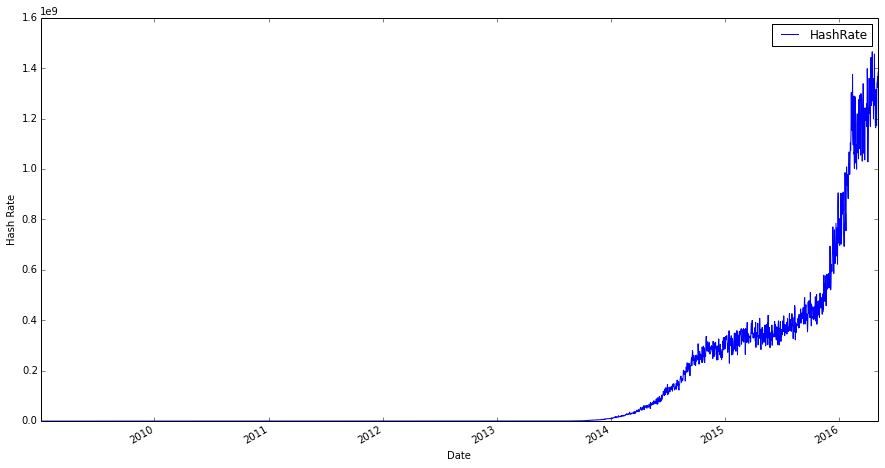
\includegraphics[width=1\linewidth]
    {gfx/hash-rate-over-time}}
  \caption{Hash Rate Over Time}
  \label{fig:hash-rate-over-time}
\end{figure}

The estimated number of giga hashes per second (billions of hashes per
second) the Bitcoin network is performing. The chart in
\autoref{fig:hash-rate-over-time} shows us how mining really started
when Bitcoin raised to its highest value around 2014, reaching more
than 1000\$ per BTC. From that point on, the processing to mining has
increased at approximately $0.2 \times 10^9$ hashes per second, and in
2016, at the same time that the Bitcoin price is starting to increase,
the hash rate started to grow at $1 \times 10^9$ hashes per second in
just a few months. 

This data-set comprises one real number data point each day, at
18:15:05, spanning from 03/01/2009 to 03/05/2016.

\begin{table}
  \myfloatalign
  %\small
  \begin{tabularx}{\textwidth}{XX}
    \toprule
    \tableheadline{Measure} & \tableheadline{Value} \\
    \midrule
    count  & $2.678000e+03$      \\
    mean   & $1.265485e+08$      \\
    median & $19063.08687085293$ \\
    std    & $2.683517e+08$      \\
    min    & $0.000000e+00$      \\
    $25$\% & $2.973922e+01$      \\
    $50$\% & $1.906309e+04$      \\
    $75$\% & $1.250993e+08$      \\
    max    & $1.465554e+09$      \\
    \bottomrule
  \end{tabularx}
  \caption{Statistical values for \textit{Hash Rate}}
  \label{tab:hash-rate}
\end{table}

\begin{figure}[bth]
  \myfloatalign
  {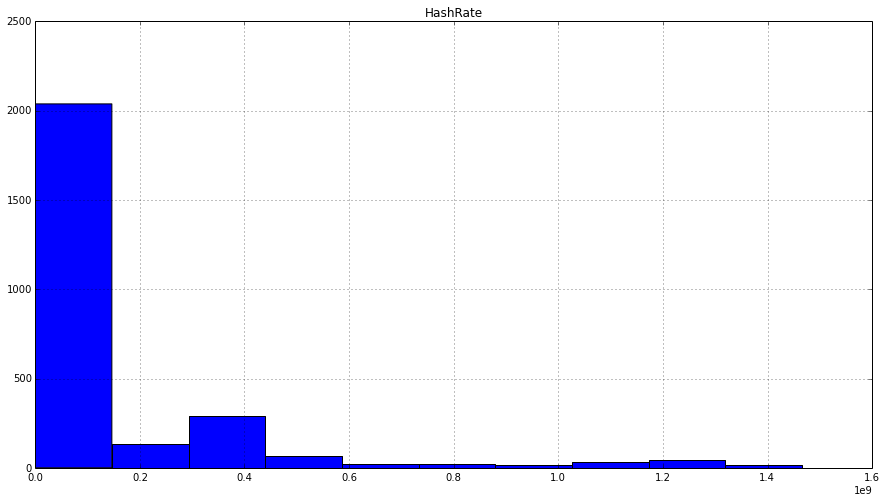
\includegraphics[width=1\linewidth]
    {gfx/hash-rate-histogram}}
  \caption{Hash Rate Histogram}
  \label{fig:hash-rate-histogram}
\end{figure}

\begin{figure}[bth]
  \myfloatalign
  {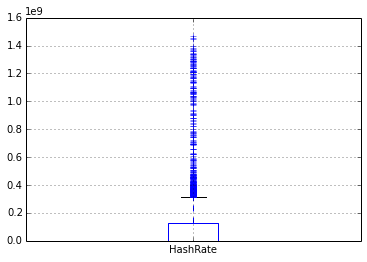
\includegraphics[width=1\linewidth]
    {gfx/hash-rate-boxplot}}
  \caption{Hash Rate Boxplot}
  \label{fig:hash-rate-boxplot}
\end{figure}

\clearpage
%----------------------------------------------------------------------

\subsection{Market Capitalization}
\label{sec:market-cap}

\begin{figure}[bth]
  \myfloatalign
  {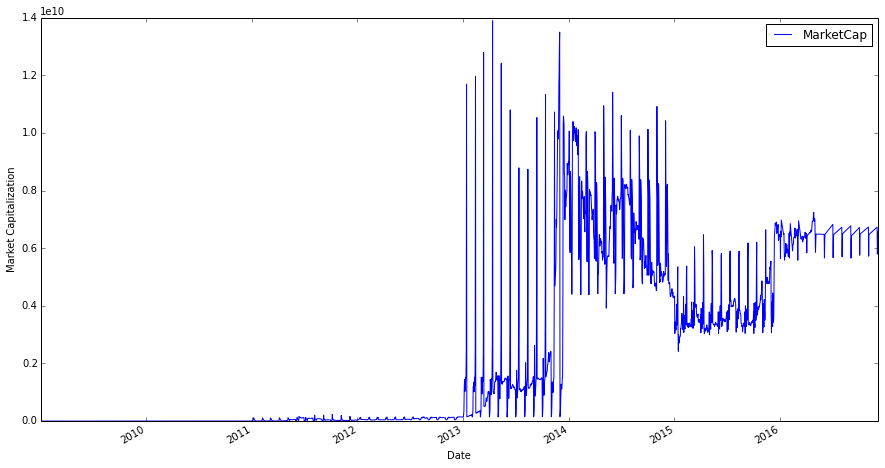
\includegraphics[width=1\linewidth]
    {gfx/market-cap-over-time}}
  \caption{Market Capitalization Over Time}
  \label{fig:market-cap-over-time}
\end{figure}

The total USD value of bitcoin supply in circulation, as calculated by
the daily average market price across major exchanges. This variable
is related to many others, starting with the Bitcoin market price,
with is virtually the same as this one, the number of transactions,
that can explain the fluctuations in the Bitcoin price and different
events. In March 9, 2011, the Bitcoin reaches parity with USD which is
shown in a timid growth in market capitalization followed by a
decrease. After that there isn't a big growth until 2013, where
several things happen, Mega, the cloud storage service, starts
accepting Bitcoins, Internet Archive starts accepting Bitcoins, a new
food service \href{PizzaForCoins.com}{PizzaForCoins.com} accepts
Bitcoins as a payment for food, CoinDesk is launched by Spotify
investor and Coinbase receives 5 million USD in funding. This, and
several other events increase the market capitalization for Bitcoin.

After that there is a decrease in market capitalization of Bitcoin,
maybe because MtGox, the largest exchange operator at the time, was
seized by The United States Department of Homeland Security.

In the second half of 2013, various events happen that can be the
cause of the raise of Bitcoin market capitalization, first, in August
6th, Bitcoin is ruled currency by a Texas judge, then in August 20th,
Bitcoin is ruled as private money in Germany, then in August 28th,
RoboCoin, a Bitcoin ATM manufacturer, starts accepting orders. This
can be the cause of the huge peek at the end of 2013 and start of
2014. There are no clear events in the Bitcoin history that explain
the period after 2014, which leads us to think that the price has been
fluctuating due to trading strategies.

This data-set comprises one real number data point each day, at
18:15:05, spanning from 03/01/2009 to 03/05/2016.

\begin{table}
  \myfloatalign
  %\small
  \begin{tabularx}{\textwidth}{XX} 
    \toprule
    \tableheadline{Measure} & \tableheadline{Value} \\
    \midrule 
    count  & $2.678000e+03$  \\
    mean   & $2.072915e+09$  \\
    median & $115624066.175$ \\
    std    & $2.879009e+09$  \\
    min    & $0.000000e+00$  \\
    $25$\% & $1.005470e+06$  \\
    $50$\% & $1.156241e+08$  \\
    $75$\% & $3.850512e+09$  \\
    max    & $1.390005e+10$  \\
    \bottomrule
  \end{tabularx}
  \caption{Statistical values for \textit{Market Capitalization}}
  \label{tab:market-cap}
\end{table}

\begin{figure}[bth]
  \myfloatalign
  {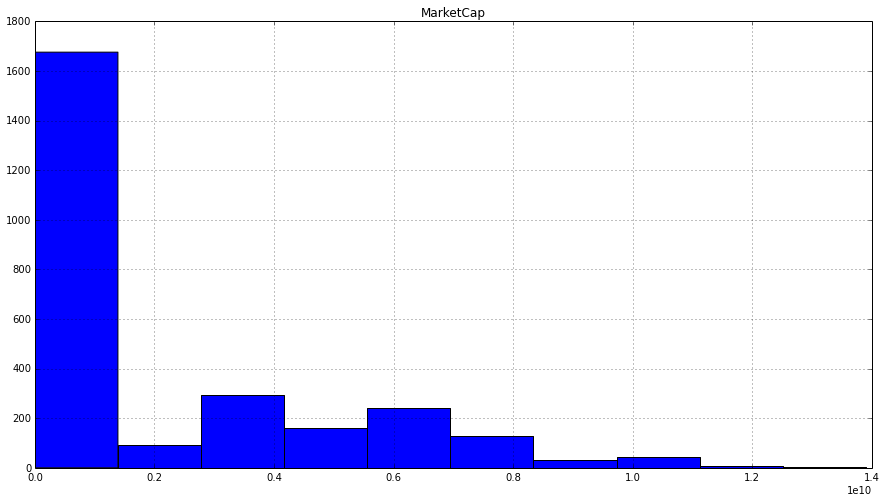
\includegraphics[width=1\linewidth]
    {gfx/market-cap-histogram}}
  \caption{Market Capitalization Histogram}
  \label{fig:market-cap-histogram}
\end{figure}

\begin{figure}[bth]
  \myfloatalign
  {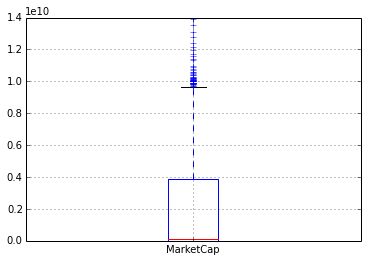
\includegraphics[width=1\linewidth]
    {gfx/market-cap-boxplot}}
  \caption{Market Capitalization Boxplot}
  \label{fig:market-cap-boxplot}
\end{figure}

\clearpage
%----------------------------------------------------------------------

\subsection{Market Price}
\label{sec:market-price}

\begin{figure}[bth]
  \myfloatalign
  {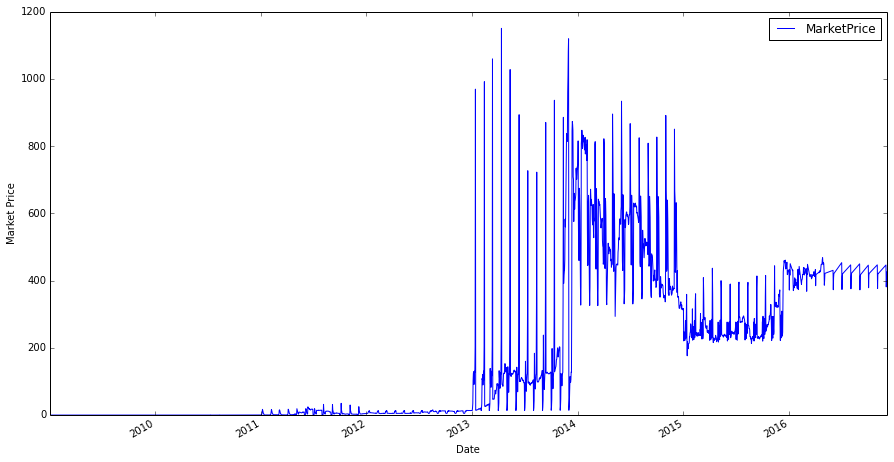
\includegraphics[width=1\linewidth]
    {gfx/market-price-over-time}}
  \caption{Market Price Over Time}
  \label{fig:market-price-over-time}
\end{figure}

Average USD market price across major Bitcoin exchanges.
\autoref{fig:market-price-over-time} is identical to the one in
\autoref{fig:market-cap-over-time} except for the scale. The same
events that produced the market capitalization fluctuation apply to
the market price. Added to that, the average market price across mayor
Bitcoin exchange operators is a variable very closely related to the
market capitalization of Bitcoin.

Is important to note how volatile is the Bitcoin average price,
ranging from nearly $0$ USD to $1100$ USD in just a year, and now, in
2016 fluctuating in a range bigger than $10$ USD on average. This
fluctuations, if predicted, can be very profitable for the trader. 

The data-set comprises one real number data point each day, at
18:15:05, spanning from 03/01/2009 to 03/05/2016.

\begin{table}
  \myfloatalign
  %\small
  \begin{tabularx}{\textwidth}{XX} 
    \toprule
    \tableheadline{Measure} & \tableheadline{Value} \\
    \midrule 
    count  & $2678.000000$ \\
    mean   & $155.924369$  \\
    median & $12.37856$    \\
    std    & $218.563332$  \\
    min    & $0.000000$    \\
    $25$\% & $0.209250$    \\
    $50$\% & $12.378560$   \\
    $75$\% & $271.335000$  \\
    max    & $1151.000000$ \\
    \bottomrule
  \end{tabularx}
  \caption{Statistical values for \textit{Market Price}}
  \label{tab:market-price}
\end{table}

\begin{figure}[bth]
  \myfloatalign
  {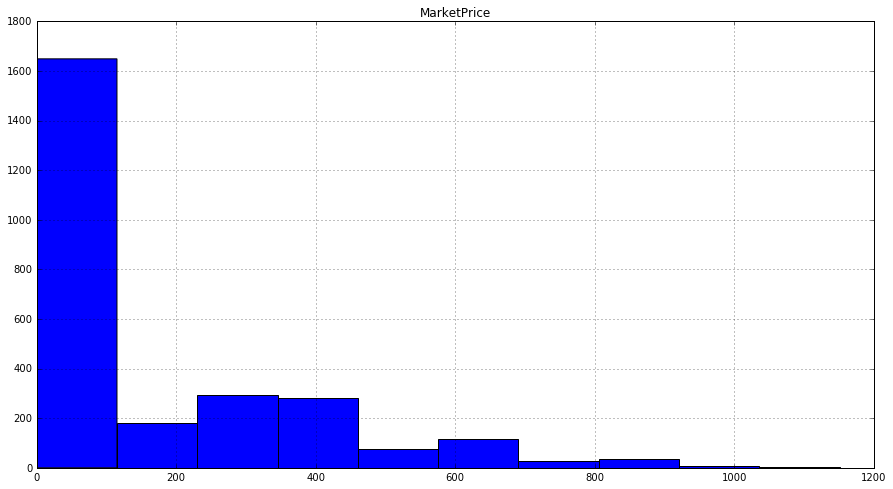
\includegraphics[width=1\linewidth]
    {gfx/market-price-histogram}}
  \caption{Market Price Histogram}
  \label{fig:market-price-histogram}
\end{figure}

\begin{figure}[bth]
  \myfloatalign
  {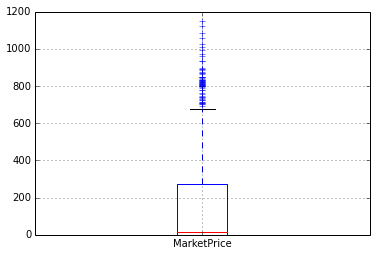
\includegraphics[width=1\linewidth]
    {gfx/market-price-boxplot}}
  \caption{Market Price Boxplot}
  \label{fig:market-price-boxplot}
\end{figure}

\clearpage
%----------------------------------------------------------------------

\subsection{Median Confirmation Time}
\label{sec:median-confirmation-time}

\begin{figure}[bth]
  \myfloatalign
  {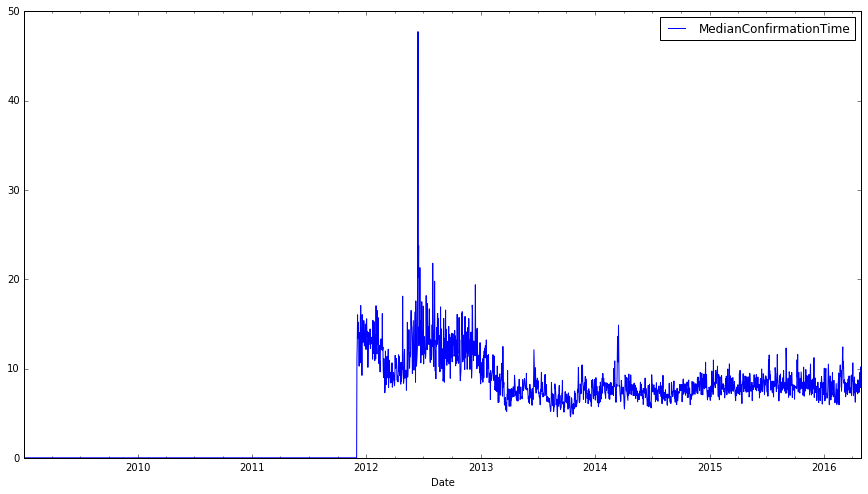
\includegraphics[width=1\linewidth]
    {gfx/median-confirmation-time-over-time}}
  \caption{Median Confirmation Time Over Time}
  \label{fig:median-confirmation-time-over-time}
\end{figure}

The median time for a transaction to be accepted into a mined block
and added to the public ledger (note: only includes transactions with
miner fees). Until the end of 2011, the confirmation time is
negligible. There is an important event that can be related to the
growth of the median confirmation time, and that is the largest
Bitcoin fee in a single transaction, in December 12, 171 Bitcoins was
paids as fee in block 157235.

If we look at \autoref{fig:median-confirmation-time-over-time} there
is a peak in mid 2012, that can coincide with the increase in number
of transactions seen in \autoref{fig:n-transactions-over-time}. After
that even though the number of transactions is growing, there is also
in increment in the hash rate, so the number of transactions can be
included in blocks thanks to the amount of miners and their processing
power.

 One real number data point each day, at 18:15:05,
spanning from 03/01/2009 to 03/05/2016.

\begin{table}
  \myfloatalign
  %\small
  \begin{tabularx}{\textwidth}{XX} 
    \toprule
    \tableheadline{Measure} & \tableheadline{Value} \\
    \midrule 
    count  & $2678.000000$ \\
    mean   & $5.385540$    \\
    median & $6.975$       \\
    std    & $4.859709$    \\
    min    & $0.000000$    \\
    $25$\% & $0.000000$    \\
    $50$\% & $6.975000$    \\
    $75$\% & $8.500000$    \\
    max    & $47.733333$   \\
    \bottomrule
  \end{tabularx}
  \caption{Statistical values for 
    \textit{Median Confirmation Time}}
  \label{tab:median-confirmation-time}
\end{table}

\begin{figure}[bth]
  \myfloatalign
  {\includegraphics[width=1\linewidth]
    {gfx/median-confirmation-time-histogram}}
  \caption{Median Confirmation Time Histogram}
  \label{fig:median-confirmation-time-histogram}
\end{figure}

\begin{figure}[bth]
  \myfloatalign
  {\includegraphics[width=1\linewidth]
    {gfx/median-confirmation-time-boxplot}}
  \caption{Median Confirmation Time Boxplot}
  \label{fig:median-confirmation-time-boxplot}
\end{figure}

\clearpage
%----------------------------------------------------------------------

\subsection{Miners Revenue}
\label{sec:miners-revenue}

\begin{figure}[bth]
  \myfloatalign
  {\includegraphics[width=1\linewidth]
    {gfx/miners-revenue-over-time}}
  \caption{Miners Revenue Over Time}
  \label{fig:miners-revenue-over-time}
\end{figure}

Total value of coinbase block rewards and transaction fees paid to
miners, expressed in USD. To understand the rewards and fees, we
include this quote, extracted the 1st of June of 2016 from
\href{https://en.bitcoin.it/wiki/Mining}{https://en.bitcoin.it/wiki/Mining}:

\textit{``When a block is discovered, the discoverer may award
  themselves a certain number of bitcoins, which is agreed-upon by
  everyone in the network. Currently this bounty is 25 bitcoins; this
  value will halve every 210,000 blocks. [...]. } 

\textit{Additionally, the miner is awarded the fees paid by users
  sending transactions. The fee is an incentive for the miner to
  include the transaction in their block. In the future, as the number
  of new bitcoins miners are allowed to create in each block dwindles,
  the fees will make up a much more important percentage of mining
  income.''}

Taking the previous quote into consideration, we know that the miner
reward is fixed, so its fluctuation will depend upon the price of the
Bitcoin itself, therefore the resemblance between miners revenue
(\autoref{fig:miners-revenue-over-time}) and Bitcoin price
(\autoref{fig:market-price-over-time}).

In 2016, the transaction fees represent a very small amount of the
BTCs of the miners revenue. We can see in
\autoref{tab:cost-per-transaction} that the average transaction has a
value of $9.727391$. On the other hand, the average number of
transactions per block $306.632248$. Thus the expected revenue due to
fees of a single miner is $9.727391 \times 306.632248 = $
$2982.7317695049683$ USD.

If we analyze the revenue thanks to the reward of discovering a block
we have that the average market price of the
Bitcoin(\autoref{tab:market-price}) is $155.924369$ USD and the reward
is $25$ BTC per block discovered, that makes an amount of $155.924369
\times 25 = 3898.109225$ USD per block discovered. Added to that, we
have to keep in mind that, as of June the $2^{nd}$, the current price
of Bitcoin is $536.99$ USD, which makes the rewards value increase to
$536.99 \times 25 = 13424.75$ USD per blocked discovered. We can
conclude that nowadays, the main source of revenues for miners is the
block discovery, but in the future, as it goes getting harder to
discover blocks, the fees will start to be an important source of
income for miners. 

This data-set comprises one real number data point each day, at
18:15:05, spanning from 03/01/2009 to 03/05/2016.

\begin{table}
  \myfloatalign
  %\small
  \begin{tabularx}{\textwidth}{XX} 
    \toprule
    \tableheadline{Measure} & \tableheadline{Value} \\
    \midrule 
    count  & $2678.000000$    \\
    mean   & $638331.424709$  \\
    median & $85611.64705$    \\
    std    & $911565.967412$  \\
    min    & $0.000000$       \\
    $25$\% & $1895.375000$    \\
    $50$\% & $85611.647050$   \\
    $75$\% & $1023087.365000$ \\
    max    & $5117346.000000$ \\
    \bottomrule
  \end{tabularx}
  \caption{Statistical values for \textit{Miners Revenue}}
  \label{tab:miners-revenue}
\end{table}

\begin{figure}[bth]
  \myfloatalign
  {\includegraphics[width=1\linewidth]
    {gfx/miners-revenue-histogram}}
  \caption{Miners Revenue Histogram}
  \label{fig:miners-revenue-histogram}
\end{figure}

\begin{figure}[bth]
  \myfloatalign
  {\includegraphics[width=1\linewidth]
    {gfx/miners-revenue-boxplot}}
  \caption{Miners Revenue Boxplot}
  \label{fig:miners-revenue-boxplot}
\end{figure}

\clearpage
%----------------------------------------------------------------------

\subsection{Network Deficit}
\label{sec:network-deficit}

\begin{figure}[bth]
  \myfloatalign
  {\includegraphics[width=1\linewidth]
    {gfx/network-deficit-over-time}}
  \caption{Network Deficit Over Time}
  \label{fig:network-deficit-over-time}
\end{figure}

Shows difference between transaction fees and cost of bitcoin mining.
One real number data point each day, at 18:15:05, spanning from
03/01/2009 to 03/05/2016.


\begin{table}
  \myfloatalign
  %\small
  \begin{tabularx}{\textwidth}{XX} 
    \toprule
    \tableheadline{Measure} & \tableheadline{Value} \\
    \midrule 
    count  & $2678.000000$ \\
    mean   & -$631395.059680$ \\
    median & -$84958.600143$ \\
    std    & $903713.147531$ \\
    min    & -$5068845.988395$ \\
    $25$\% & -$1009464.098582$ \\
    $50$\% & -$84958.600143$ \\
    $75$\% & -$1895.354052$ \\
    max    & $0.000000$ \\
    \bottomrule
  \end{tabularx}
  \caption{Statistical values for \textit{Network Deficit}}
  \label{tab:network-deficit}
\end{table}

\begin{figure}[bth]
  \myfloatalign
  {\includegraphics[width=1\linewidth]
    {gfx/network-deficit-histogram}}
  \caption{Network Deficit Histogram}
  \label{fig:network-deficit-histogram}
\end{figure}

\begin{figure}[bth]
  \myfloatalign
  {\includegraphics[width=1\linewidth]
    {gfx/network-deficit-boxplot}}
  \caption{Network Deficit Boxplot}
  \label{fig:network-deficit-boxplot}
\end{figure}

\clearpage
%----------------------------------------------------------------------

\subsection{Number of Orphaned Blocks}
\label{sec:n-orphaned-blocks}

\begin{figure}[bth]
  \myfloatalign
  {\includegraphics[width=1\linewidth]
    {gfx/n-orphaned-blocks-over-time}}
  \caption{Number of Orphaned Blocks Over Time}
  \label{fig:n-orphaned-blocks-over-time}
\end{figure}

The total number of blocks mined but ultimately not attached to the
main Bitcoin blockchain. One integer data point each day, at 18:15:05,
spanning from 03/01/2009 to 03/05/2016.

\begin{table}
  \myfloatalign
  %\small
  \begin{tabularx}{\textwidth}{XX} 
    \toprule
    \tableheadline{Measure} & \tableheadline{Value} \\
    \midrule 
    count  & $2678.000000$ \\
    mean   & $0.344287$    \\
    median & $0$           \\
    std    & $0.849656$    \\
    min    & $0.000000$    \\
    $25$\% & $0.000000$    \\
    $50$\% & $0.000000$    \\
    $75$\% & $0.000000$    \\
    max    & $7.000000$    \\
    \bottomrule
  \end{tabularx}
  \caption{Statistical values for \textit{Number of Orphaned Blocks}}
  \label{tab:n-orphaned-blocks}
\end{table}

\begin{figure}[bth]
  \myfloatalign
  {\includegraphics[width=1\linewidth]
    {gfx/n-orphaned-blocks-histogram}}
  \caption{Number of Orphaned Blocks Histogram}
  \label{fig:n-orphaned-blocks-histogram}
\end{figure}

\begin{figure}[bth]
  \myfloatalign
  {\includegraphics[width=1\linewidth]
    {gfx/n-orphaned-blocks-boxplot}}
  \caption{Number of Orphaned Blocks Boxplot}
  \label{fig:n-orphaned-blocks-boxplot}
\end{figure}

\clearpage
%----------------------------------------------------------------------

\subsection{Number of Transactions}
\label{sec:n-transactions}

\begin{figure}[bth]
  \myfloatalign
  {\includegraphics[width=1\linewidth]
    {gfx/n-transactions-over-time}}
  \caption{Number of Transactions Over Time}
  \label{fig:n-transactions-over-time}
\end{figure}

The number of daily confirmed Bitcoin transactions. One integer data
point each day, at 18:15:05, spanning from 03/01/2009 to 03/05/2016.

\begin{table}
  \myfloatalign
  %\small
  \begin{tabularx}{\textwidth}{XX} 
    \toprule
    \tableheadline{Measure} & \tableheadline{Value} \\
    \midrule 
    count  & $2678.000000$   \\
    mean   & $47255.265497$  \\
    median & $31214$         \\
    std    & $56769.848304$  \\
    min    & $0.000000$      \\
    $25$\% & $501.500000$    \\
    $50$\% & $31214.000000$  \\
    $75$\% & $69853.000000$  \\
    max    & $276448.000000$ \\
    \bottomrule
  \end{tabularx}
  \caption{Statistical values for \textit{Number of Transactions}}
  \label{tab:n-transactions}
\end{table}

\begin{figure}[bth]
  \myfloatalign
  {\includegraphics[width=1\linewidth]
    {gfx/n-transactions-histogram}}
  \caption{Number of Transactions Histogram}
  \label{fig:n-transactions-histogram}
\end{figure}

\begin{figure}[bth]
  \myfloatalign
  {\includegraphics[width=1\linewidth]
    {gfx/n-transactions-boxplot}}
  \caption{Number of Transactions Boxplot}
  \label{fig:n-transactions-boxplot}
\end{figure}

\clearpage
%----------------------------------------------------------------------

\subsection{Number of Transactions Excluding Chains Longer Than 10000}
\label{sec:n-transactions-excluding-chains-longer-than-10000}

\begin{figure}[bth]
  \myfloatalign
  {\includegraphics[width=1\linewidth]
    {gfx/n-transactions-excluding-chains-longer-than-10000-over-time}}
  \caption{Number of Transactions Excluding Chains Longer Than 10000 Over Time}
  \label{fig:n-transactions-excluding-chains-longer-than-10000-over-time}
\end{figure}

The total number of Bitcoin transactions per day excluding those part
of transaction chains longer that 10000. One integer data point each
day, at 18:15:05, spanning from 03/01/2009 to 03/05/2016.

\begin{table}
  \myfloatalign
  %\small
  \begin{tabularx}{\textwidth}{XX} 
    \toprule
    \tableheadline{Measure} & \tableheadline{Value} \\
    \midrule 
    count  & $2678.000000$   \\
    mean   & $39117.017177$  \\
    median & $22558$         \\
    std    & $46391.775343$  \\
    min    & $0.000000$      \\
    $25$\% & $501.500000$    \\
    $50$\% & $22558.000000$  \\
    $75$\% & $61130.000000$  \\
    max    & $227830.000000$ \\
    \bottomrule
  \end{tabularx}
  \caption{Statistical values for \textit{Number of Transactions
      Excluding Chains Longer Than 10000}}
  \label{tab:n-transactions-excluding-chains-longer-than-10000}
\end{table}

\begin{figure}[bth]
  \myfloatalign
  {\includegraphics[width=1\linewidth]
    {gfx/n-transactions-excluding-chains-longer-than-10000-histogram}}
  \caption{Number of Transactions Excluding Chains Longer Than 10000
    Histogram}
  \label{fig:n-transactions-excluding-chains-longer-than-10000-histogram}
\end{figure}

\begin{figure}[bth]
  \myfloatalign
  {\includegraphics[width=1\linewidth]
    {gfx/n-transactions-excluding-chains-longer-than-10000-boxplot}}
  \caption{Number of Transactions Excluding Chains Longer Than 10000
    Boxplot}
  \label{fig:n-transactions-excluding-chains-longer-than-10000-boxplot}
\end{figure}

\clearpage
%----------------------------------------------------------------------

\subsection{Number of Transactions Excluding Chains Longer Than 1000}
\label{sec:n-transactions-excluding-chains-longer-than-1000}

\begin{figure}[bth]
  \myfloatalign
  {\includegraphics[width=1\linewidth]
    {gfx/n-transactions-excluding-chains-longer-than-1000-over-time}}
  \caption{Number of Transactions Excluding Chains Longer Than 1000
    Over Time}
  \label{fig:n-transactions-excluding-chains-longer-than-1000-over-time}
\end{figure}

The total number of Bitcoin transactions per day excluding those part
of transaction chains longer that 1000. One integer data point each
day, at 18:15:05, spanning from 03/01/2009 to 03/05/2016.

\begin{table}
  \myfloatalign
  %\small
  \begin{tabularx}{\textwidth}{XX} 
    \toprule
    \tableheadline{Measure} & \tableheadline{Value} \\
    \midrule 
    count  & $2678.000000$ \\
    mean   & $32665.966019$ \\
    median & $16915$ \\
    std    & $40035.066692$ \\
    min    & $0.000000$ \\
    $25$\% & $486.250000$ \\
    $50$\% & $16915.000000$ \\
    $75$\% & $50210.750000$ \\
    max    & $206184.000000$ \\
    \bottomrule
  \end{tabularx}
  \caption{Statistical values for \textit{Number of Transactions 
      Excluding Chains Longer Than 1000}}
  \label{tab:n-transactions-excluding-chains-longer-than-1000}
\end{table}

\begin{figure}[bth]
  \myfloatalign
  {\includegraphics[width=1\linewidth]
    {gfx/n-transactions-excluding-chains-longer-than-1000-histogram}}
  \caption{Number of Transactions Excluding Chains Longer Than 1000
    Histogram}
  \label{fig:n-transactions-excluding-chains-longer-than-1000-histogram}
\end{figure}

\begin{figure}[bth]
  \myfloatalign
  {\includegraphics[width=1\linewidth]
    {gfx/n-transactions-excluding-chains-longer-than-1000-boxplot}}
  \caption{Number of Transactions Excluding Chains Longer Than 1000
    Boxplot}
  \label{fig:n-transactions-excluding-chains-longer-than-1000-boxplot}
\end{figure}

\clearpage
%----------------------------------------------------------------------

\subsection{Number of Transactions Excluding Chains Longer Than 100}
\label{sec:n-transactions-excluding-chains-longer-than-100}

\begin{figure}[bth]
  \myfloatalign
  {\includegraphics[width=1\linewidth]
    {gfx/n-transactions-excluding-chains-longer-than-100-over-time}}
  \caption{Number of Transactions Excluding Chains Longer Than 100
    Over Time}
  \label{fig:n-transactions-excluding-chains-longer-than-100-over-time}
\end{figure}

The total number of Bitcoin transactions per day excluding those part
of long transaction chains. There are many legitimate reasons to
create long transaction chains; however, they may also be caused by
coin mixing or possible attempts to manipulate transaction volume. One
integer data point each day, at 18:15:05, spanning from 03/01/2009 to
03/05/2016.

\begin{table}
  \myfloatalign
  %\small
  \begin{tabularx}{\textwidth}{XX} 
    \toprule
    \tableheadline{Measure} & \tableheadline{Value} \\
    \midrule 
    count  & $2678.000000$   \\
    mean   & $26050.881255$  \\
    median & $12810$         \\
    std    & $32164.862369$  \\
    min    & $0.000000$      \\
    $25$\% & $426.250000$    \\
    $50$\% & $12810.000000$  \\
    $75$\% & $39936.750000$  \\
    max    & $187035.000000$ \\
    \bottomrule
  \end{tabularx}
  \caption{Statistical values for \textit{Number of Transactions 
      Excluding Chains Longer Than 100}}
  \label{tab:n-transactions-excluding-chains-longer-than-100}
\end{table}

\begin{figure}[bth]
  \myfloatalign
  {\includegraphics[width=1\linewidth]
    {gfx/n-transactions-excluding-chains-longer-than-100-histogram}}
  \caption{Number of Transactions Excluding Chains Longer Than 100
    Histogram}
  \label{fig:n-transactions-excluding-chains-longer-than-100-histogram}
\end{figure}

\begin{figure}[bth]
  \myfloatalign
  {\includegraphics[width=1\linewidth]
    {gfx/n-transactions-excluding-chains-longer-than-100-boxplot}}
  \caption{Number of Transactions Excluding Chains Longer Than 100
    Boxplot}
  \label{fig:n-transactions-excluding-chains-longer-than-100-boxplot}
\end{figure}

\clearpage
%----------------------------------------------------------------------

\subsection{Number of Transactions Excluding Chains Longer Than 10}
\label{sec:n-transactions-excluding-chains-longer-than-10}

\begin{figure}[bth]
  \myfloatalign
  {\includegraphics[width=1\linewidth]
    {gfx/n-transactions-excluding-chains-longer-than-10-over-time}}
  \caption{Number of Transactions Excluding Chains Longer Than 10
    Over Time}
  \label{fig:n-transactions-excluding-chains-longer-than-10-over-time}
\end{figure}

The total number of Bitcoin transactions per day excluding those part
of transaction chains longer that 10. One integer data point each day,
at 18:15:05, spanning from 03/01/2009 to 03/05/2016.

\begin{table}
  \myfloatalign
  %\small
  \begin{tabularx}{\textwidth}{XX} 
    \toprule
    \tableheadline{Measure} & \tableheadline{Value} \\
    \midrule 
    count  & $2678.000000$   \\
    mean   & $15589.578790$  \\
    median & $7115$          \\
    std    & $20367.504877$  \\
    min    & $0.000000$      \\
    $25$\% & $337.000000$    \\
    $50$\% & $7115.000000$   \\
    $75$\% & $23695.500000$  \\
    max    & $157002.000000$ \\
    \bottomrule
  \end{tabularx}
  \caption{Statistical values for \textit{Number of Transactions 
      Excluding Chains Longer Than 10}}
  \label{tab:n-transactions-excluding-chains-longer-than-10}
\end{table}

\begin{figure}[bth]
  \myfloatalign
  {\includegraphics[width=1\linewidth]
    {gfx/n-transactions-excluding-chains-longer-than-10-histogram}}
  \caption{Number of Transactions Excluding Chains Longer Than 10
    Histogram}
  \label{fig:n-transactions-excluding-chains-longer-than-10-histogram}
\end{figure}

\begin{figure}[bth]
  \myfloatalign
  {\includegraphics[width=1\linewidth]
    {gfx/n-transactions-excluding-chains-longer-than-10-boxplot}}
  \caption{Number of Transactions Excluding Chains Longer Than 10
    Boxplot}
  \label{fig:n-transactions-excluding-chains-longer-than-10-boxplot}
\end{figure}

\clearpage
%----------------------------------------------------------------------

\subsection{Number of Transactions Excluding Popular}
\label{sec:n-transactions-excluding-popular}

\begin{figure}[bth]
  \myfloatalign
  {\includegraphics[width=1\linewidth]
    {gfx/n-transactions-excluding-popular-over-time}}
  \caption{Number of Transactions Excluding Popular
    Over Time}
  \label{fig:n-transactions-excluding-popular-over-time}
\end{figure}

The total number of Bitcoin transactions, excluding those involving
any of the network's 100 most popular addresses. One integer data
point each day, at 18:15:05, spanning from 03/01/2009 to 03/05/2016.

\begin{table}
  \myfloatalign
  %\small
  \begin{tabularx}{\textwidth}{XX} 
    \toprule
    \tableheadline{Measure} & \tableheadline{Value} \\
    \midrule 
    count  & $2678.000000$   \\
    mean   & $40400.536968$  \\
    median & $12597.5$       \\
    std    & $55357.260528$  \\
    min    & $0.000000$      \\
    $25$\% & $501.500000$    \\
    $50$\% & $12597.500000$  \\
    $75$\% & $63434.250000$  \\
    max    & $262461.000000$ \\
    \bottomrule
  \end{tabularx}
  \caption{Statistical values for \textit{Number of Transactions 
      Excluding Popular}}
  \label{tab:n-transactions-excluding-popular}
\end{table}

\begin{figure}[bth]
  \myfloatalign
  {\includegraphics[width=1\linewidth]
    {gfx/n-transactions-excluding-popular-histogram}}
  \caption{Number of Transactions Excluding Popular
    Histogram}
  \label{fig:n-transactions-excluding-popular-histogram}
\end{figure}

\begin{figure}[bth]
  \myfloatalign
  {\includegraphics[width=1\linewidth]
    {gfx/n-transactions-excluding-popular-boxplot}}
  \caption{Number of Transactions Excluding Popular
    Boxplot}
  \label{fig:n-transactions-excluding-popular-boxplot}
\end{figure}

\clearpage
%----------------------------------------------------------------------

\subsection{Number of Transactions Per Block}
\label{sec:n-transactions-per-block}

\begin{figure}[bth]
  \myfloatalign
  {\includegraphics[width=1\linewidth]
    {gfx/n-transactions-per-block-over-time}}
  \caption{Number of Transactions Per Block
    Over Time}
  \label{fig:n-transactions-per-block-over-time}
\end{figure}

The average number of transactions per block. One integer data point
each day, at 18:15:05, spanning from 03/01/2009 to 28/04/2016.

\begin{table}
  \myfloatalign
  %\small
  \begin{tabularx}{\textwidth}{XX} 
    \toprule
    \tableheadline{Measure} & \tableheadline{Value} \\
    \midrule 
    count  & $2673$ \\
    mean   & $306.632248$  \\
    median & $205$         \\
    std    & $377.986965$  \\
    min    & $1$    \\
    $25$\% & $2$    \\
    $50$\% & $205$  \\
    $75$\% & $435$  \\
    max    & $2036$ \\
    \bottomrule
  \end{tabularx}
  \caption{Statistical values for \textit{Number of Transactions 
      Per Block}}
  \label{tab:n-transactions-per-block}
\end{table}

\begin{figure}[bth]
  \myfloatalign
  {\includegraphics[width=1\linewidth]
    {gfx/n-transactions-per-block-histogram}}
  \caption{Number of Transactions Per Block
    Histogram}
  \label{fig:n-transactions-per-block-histogram}
\end{figure}

\begin{figure}[bth]
  \myfloatalign
  {\includegraphics[width=1\linewidth]
    {gfx/n-transactions-per-block-boxplot}}
  \caption{Number of Transactions Per Block
    Boxplot}
  \label{fig:n-transactions-per-block-boxplot}
\end{figure}

\clearpage
%---------------------------------------------------------------------- 

\subsection{Number of Total Transactions}
\label{sec:n-transactions-total}

\begin{figure}[bth]
  \myfloatalign
  {\includegraphics[width=1\linewidth]
    {gfx/n-transactions-total-over-time}}
  \caption{Number of Total Transactions
    Over Time}
  \label{fig:n-transactions-total-over-time}
\end{figure}

Total number of transactions. One integer data point each day, at
18:15:05, spanning from 03/01/2009 to 03/05/2016.

\begin{table}
  \myfloatalign
  %\small
  \begin{tabularx}{\textwidth}{XX} 
    \toprule
    \tableheadline{Measure} & \tableheadline{Value} \\
    \midrule 
    count  & $2.678000e+03$ \\
    mean   & $2.491078e+07$ \\
    median & $6685067$      \\
    std    & $3.308262e+07$ \\
    min    & $1.000000e+00$ \\
    $25$\% & $1.384448e+05$ \\
    $50$\% & $6.685067e+06$ \\
    $75$\% & $4.191287e+07$ \\
    max    & $1.265496e+08$ \\
    \bottomrule
  \end{tabularx}
  \caption{Statistical values for \textit{Number of Total
      Transactions}}
  \label{tab:n-transactions-total}
\end{table}

\begin{figure}[bth]
  \myfloatalign
  {\includegraphics[width=1\linewidth]
    {gfx/n-transactions-total-histogram}}
  \caption{Number of Total Transactions
    Histogram}
  \label{fig:n-transactions-total-histogram}
\end{figure}

\begin{figure}[bth]
  \myfloatalign
  {\includegraphics[width=1\linewidth]
    {gfx/n-transactions-total-boxplot}}
  \caption{Number of Total Transactions
    Boxplot}
  \label{fig:n-transactions-total-boxplot}
\end{figure}

\clearpage
%---------------------------------------------------------------------- 

\subsection{Number of Unique Addresses}
\label{sec:n-unique-addresses}

\begin{figure}[bth]
  \myfloatalign
  {\includegraphics[width=1\linewidth]
    {gfx/n-unique-addresses-over-time}}
  \caption{Number of Unique Addresses
    Over Time}
  \label{fig:n-unique-addresses-over-time}
\end{figure}

The total number of unique addresses used on the Bitcoin blockchain.
One integer data point each day, at 18:15:05, spanning from 03/01/2009
to 03/05/2016.

\begin{table}
  \myfloatalign
  %\small
  \begin{tabularx}{\textwidth}{XX} 
    \toprule
    \tableheadline{Measure} & \tableheadline{Value} \\
    \midrule 
    count &        $2678.000000$ \\
    mean &        $86921.616878$ \\
    median &        $29205.5$ \\
    std &        $112219.880994$ \\
    min &             $0.000000$ \\
    $25$\% &          $609.250000$ \\
    $50$\% &        $29205.500000$ \\
    $75$\% &       $152308.500000$ \\
    max &        $483756.000000$ \\
    \bottomrule
  \end{tabularx}
  \caption{Statistical values for \textit{Number of Unique Addresses}}
  \label{tab:n-unique-addresses}
\end{table}

\begin{figure}[bth]
  \myfloatalign
  {\includegraphics[width=1\linewidth]
    {gfx/n-unique-addresses-histogram}}
  \caption{Number of Unique Addresses
    Histogram}
  \label{fig:n-unique-addresses-histogram}
\end{figure}

\begin{figure}[bth]
  \myfloatalign
  {\includegraphics[width=1\linewidth]
    {gfx/n-unique-addresses-boxplot}}
  \caption{Number of Unique Addresses
    Boxplot}
  \label{fig:n-unique-addresses-boxplot}
\end{figure}

\clearpage
%--------------------------------------------------------------------- 

\subsection{Output Volume}
\label{sec:output-volume}

\begin{figure}[bth]
  \myfloatalign
  {\includegraphics[width=1\linewidth]
    {gfx/output-volume-over-time}}
  \caption{Output Volume
    Over Time}
  \label{fig:output-volume-over-time}
\end{figure}

The total value of all transaction outputs per day (includes coins
returned to the sender as change). One real number data point each
day, at 18:15:05, spanning from 03/01/2009 to 03/05/2016.

\begin{table}
  \myfloatalign
  %\small
  \begin{tabularx}{\textwidth}{XX} 
    \toprule
    \tableheadline{Measure} & \tableheadline{Value} \\
    \midrule 
    count &      $2679.000000$ \\
    mean &    $1134859.870780$ \\
    median &       $661019.796765$ \\
    std &     $2333431.889695$ \\
    min &           $0.000000$ \\
    $25$\% &      $73233.013445$ \\
    $50$\% &     $661019.796765$ \\
    $75$\% &    $1286432.155226$ \\
    max &    $45992222.558034$ \\
    \bottomrule
  \end{tabularx}
  \caption{Statistical values for \textit{Output Volume}}
  \label{tab:output-volume}
\end{table}

\begin{figure}[bth]
  \myfloatalign
  {\includegraphics[width=1\linewidth]
    {gfx/output-volume-histogram}}
  \caption{Output Volume
    Histogram}
  \label{fig:output-volume-histogram}
\end{figure}

\begin{figure}[bth]
  \myfloatalign
  {\includegraphics[width=1\linewidth]
    {gfx/output-volume-boxplot}}
  \caption{Output Volume
    Boxplot}
  \label{fig:output-volume-boxplot}
\end{figure}

\clearpage
%--------------------------------------------------------------------- 

\subsection{Standard Output Volume Poors 500}
\label{sec:standard-and-poors-500}

\begin{figure}[bth]
  \myfloatalign
  {\includegraphics[width=1\linewidth]
    {gfx/standard-and-poors-500-over-time}}
  \caption{Standard Output Volume Poors 500
    Over Time}
  \label{fig:standard-and-poors-500-over-time}
\end{figure}

Six real data point entry each day, spanning from 03/01/1950 to
09/05/2016. The variable names are \textit{Open}, \textit{High},
\textit{Low}, \textit{Close}, \textit{Volume}, \textit{Adj} and
\textit{Close}, representing different characteristics of the index
price.

From the Wikipedia: ``\textit{The Standard \& Poor's 500, often
  abbreviated as the S\&P 500, or just "the S\&P", is an American
  stock market index based on the market capitalizations of 500 large
  companies having common stock listed on the NYSE or NASDAQ. The S\&P
  500 index components and their weightings are determined by S\&P Dow
  Jones Indices. It differs from other U.S. stock market indices, such
  as the Dow Jones Industrial Average or the Nasdaq Composite index,
  because of its diverse constituency and weighting methodology. It is
  one of the most commonly followed equity indices, and many consider
  it one of the best representations of the U.S. stock market, and a
  bellwether for the U.S. economy. The National Bureau of Economic
  Research has classified common stocks as a leading indicator of
  business cycles.}''

\begin{table}
  \myfloatalign
  \tiny
  \begin{tabularx}{\textwidth}{XXXXXXX} 
    \toprule
    \tableheadline{Measure} & \tableheadline{Open} &
    \tableheadline{High} & \tableheadline{Low} & \tableheadline{Close}
    & \tableheadline{Volume} & \tableheadline{Adj Close}\\
    \midrule 
    count  & $16695$       & $16695$       & $16695$       & $16695$       & $1.669500e+04$ & $16695$       \\
    mean   & $492.103240$  & $495.207861$  & $488.827423$  & $492.221084$  & $8.157494e+08$ & $492.221084$  \\
    median & $150.910004$  & $151.619995$  & $150.240005$  & $151.039993$  & $75180000$     & $151.039993$  \\
    std    & $566.001594$  & $569.347411$  & $562.382420$  & $566.107954$  & $1.478957e+09$ & $566.107954$  \\
    min    & $16.660000$   & $16.660000$   & $16.660000$   & $16.660000$   & $6.800000e+05$ & $16.660000$   \\
    $25$\% & $84.099998$   & $84.765000$   & $83.459999$   & $84.099998$   & $7.805000e+06$ & $84.099998$   \\
    $50$\% & $150.910004$  & $151.619995$  & $150.240005$  & $151.039993$  & $7.518000e+07$ & $151.039993$  \\
    $75$\% & $974.309998$  & $983.190002$  & $964.844971$  & $974.904999$  & $8.428500e+08$ & $974.904999$  \\
    max    & $2130.360107$ & $2134.719971$ & $2126.060059$ & $2130.820068$ & $1.145623e+10$ & $2130.820068$ \\
    \bottomrule
  \end{tabularx}
  \caption{Statistical values for \textit{Standard Output Volume Poors 500}}
  \label{tab:standard-and-poors-500}
\end{table}

\begin{figure}[bth]
  \myfloatalign
  {\includegraphics[width=1\linewidth]
    {gfx/standard-and-poors-500-histogram}}
  \caption{Standard Output Volume Poors 500
    Histogram}
  \label{fig:standard-and-poors-500-histogram}
\end{figure}

\begin{figure}[bth]
  \myfloatalign
  {\includegraphics[width=1\linewidth]
    {gfx/standard-and-poors-500-boxplot}}
  \caption{Standard Output Volume Poors 500
    Boxplot}
  \label{fig:standard-and-poors-500-boxplot}
\end{figure}

Due to the difference in scale of the variable \textit{Volume}
compared to the rest of variables it's not possible to see their
boxplots in \autoref{fig:standard-and-poors-500-boxplot}. We need
another boxplot, seen in
\autoref{fig:standard-and-poors-500-rest-boxplot}, for the rest of the
variables to be seen clearly.

\begin{figure}[bth]
  \myfloatalign
  {\includegraphics[width=1\linewidth]
    {gfx/standard-and-poors-500-rest-boxplot}}
  \caption{Standard Output Volume Poors 500
    Rest of Variables Boxplot}
  \label{fig:standard-and-poors-500-rest-boxplot}
\end{figure}

\clearpage
%--------------------------------------------------------------------- 

\subsection{Total Bitcoins}
\label{sec:total-bitcoins}

\begin{figure}[bth]
  \myfloatalign
  {\includegraphics[width=1\linewidth]
    {gfx/total-bitcoins-over-time}}
  \caption{Total Bitcoins
    Over Time}
  \label{fig:total-bitcoins-over-time}
\end{figure}

The total number of bitcoins that have already been mined; in other
words, the current supply of bitcoins on the network. One integer data
point each day, at 18:15:05, spanning from 03/01/2009 to 03/05/2016.

\begin{table}
  \myfloatalign
  %\small
  \begin{tabularx}{\textwidth}{XX} 
    \toprule
    \tableheadline{Measure} & \tableheadline{Value} \\
    \midrule 
    count  & $2.678000e+03$ \\
    mean   & $8.723580e+06$ \\
    median & $9849250.0$    \\
    std    & $4.819287e+06$ \\
    min    & $5.000000e+01$ \\
    $25$\% & $4.472438e+06$ \\
    $50$\% & $9.849250e+06$ \\
    $75$\% & $1.297915e+07$ \\
    max    & $1.550142e+07$ \\
    \bottomrule
  \end{tabularx}
  \caption{Statistical values for \textit{Total Bitcoins}}
  \label{tab:total-bitcoins}
\end{table}

\begin{figure}[bth]
  \myfloatalign
  {\includegraphics[width=1\linewidth]
    {gfx/total-bitcoins-histogram}}
  \caption{Total Bitcoins
    Histogram}
  \label{fig:total-bitcoins-histogram}
\end{figure}

\begin{figure}[bth]
  \myfloatalign
  {\includegraphics[width=1\linewidth]
    {gfx/total-bitcoins-boxplot}}
  \caption{Total Bitcoins
    Boxplot}
  \label{fig:total-bitcoins-boxplot}
\end{figure}

\clearpage
%--------------------------------------------------------------------- 

\subsection{Trade Volume}
\label{sec:trade-volume}

\begin{figure}[bth]
  \myfloatalign
  {\includegraphics[width=1\linewidth]
    {gfx/trade-volume-over-time}}
  \caption{Trade Volume
    Over Time}
  \label{fig:trade-volume-over-time}
\end{figure}

The total USD value of trading volume on major bitcoin exchanges. One
real number data point each day, at 18:15:05, spanning from 03/01/2009
to 03/05/2016.

\begin{table}
  \myfloatalign
  %\small
  \begin{tabularx}{\textwidth}{XX} 
    \toprule
    \tableheadline{Measure} & \tableheadline{Value} \\
    \midrule 
    count  & $2.678000e+03$  \\
    mean   & $2.768062e+06$  \\
    median & $529334.610415$ \\
    std    & $5.819032e+06$  \\
    min    & $0.000000e+00$  \\
    $25$\% & $1.341996e+03$  \\
    $50$\% & $5.293346e+05$  \\
    $75$\% & $3.014521e+06$  \\
    max    & $7.205049e+07$  \\
    \bottomrule
  \end{tabularx}
  \caption{Statistical values for \textit{Trade Volume}}
  \label{tab:trade-volume}
\end{table}

\begin{figure}[bth]
  \myfloatalign
  {\includegraphics[width=1\linewidth]
    {gfx/trade-volume-histogram}}
  \caption{Trade Volume
    Histogram}
  \label{fig:trade-volume-histogram}
\end{figure}

\begin{figure}[bth]
  \myfloatalign
  {\includegraphics[width=1\linewidth]
    {gfx/trade-volume-boxplot}}
  \caption{Trade Volume
    Boxplot}
  \label{fig:trade-volume-boxplot}
\end{figure}

\clearpage
%--------------------------------------------------------------------- 

\subsection{Transaction Fees}
\label{sec:transaction-fees}

\begin{figure}[bth]
  \myfloatalign
  {\includegraphics[width=1\linewidth]
    {gfx/transaction-fees-over-time}}
  \caption{Transaction Fees
    Over Time}
  \label{fig:transaction-fees-over-time}
\end{figure}

The total value of all transaction fees paid to miners (not including
the coinbase value of block rewards) in BTC. One real number data
point each day, at 18:15:05, spanning from 03/01/2009 to 03/05/2016.

\begin{table}
  \myfloatalign
  %\small
  \begin{tabularx}{\textwidth}{XX} 
    \toprule
    \tableheadline{Measure} & \tableheadline{Value} \\
    \midrule 
    count  & $2678.000000$ \\
    mean   & $16.273161$   \\
    median & $12.23832$    \\
    std    & $20.839539$   \\
    min    & $0.000000$    \\
    $25$\% & $0.070599$    \\
    $50$\% & $12.238320$   \\
    $75$\% & $25.172616$   \\
    max    & $336.577055$  \\
    \bottomrule
  \end{tabularx}
  \caption{Statistical values for \textit{Transaction Fees}}
  \label{tab:transaction-fees}
\end{table}

\begin{figure}[bth]
  \myfloatalign
  {\includegraphics[width=1\linewidth]
    {gfx/transaction-fees-histogram}}
  \caption{Transaction Fees
    Histogram}
  \label{fig:transaction-fees-histogram}
\end{figure}

\begin{figure}[bth]
  \myfloatalign
  {\includegraphics[width=1\linewidth]
    {gfx/transaction-fees-boxplot}}
  \caption{Transaction Fees
    Boxplot}
  \label{fig:transaction-fees-boxplot}
\end{figure}

\clearpage
%--------------------------------------------------------------------- 

\subsection{Transaction Fees USD}
\label{sec:transaction-fees-usd}

\begin{figure}[bth]
  \myfloatalign
  {\includegraphics[width=1\linewidth]
    {gfx/transaction-fees-usd-over-time}}
  \caption{Transaction Fees USD
    Over Time}
  \label{fig:transaction-fees-usd-over-time}
\end{figure}

The total value of all transaction fees paid to miners (not including
the coinbase value of block rewards) in USD. One real number data
point each day, at 18:15:05, spanning from 03/01/2009 to 03/05/2016.

\begin{table}
  \myfloatalign
  %\small
  \begin{tabularx}{\textwidth}{XX} 
    \toprule
    \tableheadline{Measure} & \tableheadline{Value} \\
    \midrule 
    count  & $2678.000000$   \\
    mean   & $3506.944567$   \\
    median & $274.790467$    \\
    std    & $6026.088862$   \\
    min    & $0.000000$      \\
    $25$\% & $0.002192$      \\
    $50$\% & $274.790467$    \\
    $75$\% & $5384.674418$   \\
    max    & $157676.252853$ \\
    \bottomrule
  \end{tabularx}
  \caption{Statistical values for \textit{Transaction Fees USD}}
  \label{tab:transaction-fees-usd}
\end{table}

\begin{figure}[bth]
  \myfloatalign
  {\includegraphics[width=1\linewidth]
    {gfx/transaction-fees-usd-histogram}}
  \caption{Transaction Fees USD
    Histogram}
  \label{fig:transaction-fees-usd-histogram}
\end{figure}

\begin{figure}[bth]
  \myfloatalign
  {\includegraphics[width=1\linewidth]
    {gfx/transaction-fees-usd-boxplot}}
  \caption{Transaction Fees USD
    Boxplot}
  \label{fig:transaction-fees-usd-boxplot}
\end{figure}

\clearpage
%--------------------------------------------------------------------- 

\subsection{Transactions/Trade Ratio}
\label{sec:tx-trade-ratio}

\begin{figure}[bth]
  \myfloatalign
  {\includegraphics[width=1\linewidth]
    {gfx/tx-trade-ratio-over-time}}
  \caption{Transactions/Trade Ratio
    Over Time}
  \label{fig:tx-trade-ratio-over-time}
\end{figure}

Chart showing the relationship between BTC transaction volume and USD
exchange volume. One real number data point each day, at 18:15:0,
spanning from 03/01/2009 to 03/05/2016.

\begin{table}
  \myfloatalign
  %\small
  \begin{tabularx}{\textwidth}{XX} 
    \toprule
    \tableheadline{Measure} & \tableheadline{Value} \\
    \midrule 
    count  & $2679.000000$ \\
    mean   & $10.863982$   \\
    median & $5.164688$    \\
    std    & $16.936518$   \\
    min    & $0.000000$    \\
    $25$\% & $1.099395$    \\
    $50$\% & $5.164688$    \\
    $75$\% & $13.101565$   \\
    max    & $224.065347$  \\
    \bottomrule
  \end{tabularx}
  \caption{Statistical values for \textit{Transactions/Trade Ratio}}
  \label{tab:tx-trade-ratio}
\end{table}

\begin{figure}[bth]
  \myfloatalign
  {\includegraphics[width=1\linewidth]
    {gfx/tx-trade-ratio-histogram}}
  \caption{Transactions/Trade Ratio
    Histogram}
  \label{fig:tx-trade-ratio-histogram}
\end{figure}

\begin{figure}[bth]
  \myfloatalign
  {\includegraphics[width=1\linewidth]
    {gfx/tx-trade-ratio-boxplot}}
  \caption{Transactions/Trade Ratio
    Boxplot}
  \label{fig:tx-trade-ratio-boxplot}
\end{figure}

\clearpage
%--------------------------------------------------------------------- 

\subsection{Wikipedia Trend for Bitcoin}
\label{sec:wikipedia-trend-for-bitcoin}

\begin{figure}[bth]
  \myfloatalign
  {\includegraphics[width=1\linewidth]
    {gfx/wikipedia-trend-for-bitcoin-over-time}}
  \caption{Wikipedia Trend for Bitcoin
    Over Time}
  \label{fig:wikipedia-trend-for-bitcoin-over-time}
\end{figure}

The particular trend used in this case is the page views of the
Bitcoin article in the English version of Wikipedia. There are more
advanced trends that get information from not only the views, but the
number of edits of an article, the lines added or substracted, the
number of unique editors, etc...

We have a daily integer entry dataset ranging from 01/01/2008 till
24/05/2016.

\begin{table}
  \myfloatalign
  %\small
  \begin{tabularx}{\textwidth}{XX} 
    \toprule
    \tableheadline{Measure} & \tableheadline{Value} \\
    \midrule 
    count  & $3067.000000$   \\
    mean   & $7258.160091$   \\
    median & $3093.0$        \\
    std    & $24458.410959$  \\
    min    & $0.000000$      \\
    $25$\% & $16.000000$     \\
    $50$\% & $3093.000000$   \\
    $75$\% & $8044.500000$   \\
    max    & $923659.000000$ \\
    \bottomrule
  \end{tabularx}
  \caption{Statistical values for \textit{Wikipedia Trend for Bitcoin}}
  \label{tab:wikipedia-trend-for-bitcoin}
\end{table}

\begin{figure}[bth]
  \myfloatalign
  {\includegraphics[width=1\linewidth]
    {gfx/wikipedia-trend-for-bitcoin-histogram}}
  \caption{Wikipedia Trend for Bitcoin
    Histogram}
  \label{fig:wikipedia-trend-for-bitcoin-histogram}
\end{figure}

\begin{figure}[bth]
  \myfloatalign
  {\includegraphics[width=1\linewidth]
    {gfx/wikipedia-trend-for-bitcoin-boxplot}}
  \caption{Wikipedia Trend for Bitcoin
    Boxplot}
  \label{fig:wikipedia-trend-for-bitcoin-boxplot}
\end{figure}

\clearpage
%--------------------------------------------------------------------- 

After analyzing the date span of each variable, we conclude that the
interesction of all the sets is in the range between 03/01/2009 and
28/04/2016.

%\enlargethispage{2cm}

%------------------------------------------------

%%% Local Variables:
%%% mode: latex
%%% TeX-master: "../main"
%%% End:


\cleardoublepage % Empty page before the start of the next part

%----------------------------------------------------------------------
%	THESIS CONTENT - APPENDICES
%----------------------------------------------------------------------

% \appendix

% \part{Appendix} % New part of the thesis for the appendix

% % Appendix A

\chapter{Appendix Test}

%----------------------------------------------------------------------------------------

\lipsum[13-14]

%----------------------------------------------------------------------------------------

\section{Appendix Section Test}
\lipsum[15]

\graffito{More dummy text}
\lipsum[16]

%----------------------------------------------------------------------------------------

\section{Another Appendix Section Test}
\lipsum[17]

\begin{table}
\myfloatalign
\begin{tabularx}{\textwidth}{Xll} \toprule
\tableheadline{labitur bonorum pri no} & \tableheadline{que vista}
& \tableheadline{human} \\ \midrule
fastidii ea ius & germano &  demonstratea \\
suscipit instructior & titulo & personas \\
\midrule
quaestio philosophia & facto & demonstrated \\
\bottomrule
\end{tabularx}
\caption[Autem usu id]{Autem usu id.}
\label{tab:moreexample}
\end{table}

\lipsum[18]

There is also a useless Pascal listing below: \autoref{lst:useless}.

\begin{lstlisting}[float=b,language=Pascal,frame=tb,caption={A floating example (\texttt{listings} manual)},label=lst:useless]
for i:=maxint downto 0 do
begin
{ do nothing }
end;
\end{lstlisting} % Appendix A
%% Appendix X

\chapter{Appendix Title}

%----------------------------------------------------------------------------------------

% Content begins here % Appendix B - empty template

%----------------------------------------------------------------------
%	POST-CONTENT THESIS PAGES
%----------------------------------------------------------------------

\cleardoublepage% Bibliography

\label{app:bibliography} % Reference the bibliography elsewhere with
                         % \autoref{app:bibliography} 

\manualmark % Work-around to have small caps also here in the headline 
\markboth{\spacedlowsmallcaps{\bibname}}{\spacedlowsmallcaps{\bibname}}
% Work-around to have small caps also 
%\phantomsection
\refstepcounter{dummy}

\addtocontents{toc}{\protect\vspace{\beforebibskip}} % Place the
                                % bibliography slightly below the rest
                                % of the document content in the table
                                % of contents 
\addcontentsline{toc}{chapter}{\tocEntry{\bibname}}

\printbibliography % Bibliography

\cleardoublepage% Declaration

\refstepcounter{dummy}
\pdfbookmark[0]{Declaration}{declaration} % Bookmark name visible in a PDF viewer

\chapter*{Declaration} % Declaration section text

\thispagestyle{empty}

Put your declaration here.
\bigskip
 
\noindent\textit{\myLocation, \myTime}

\smallskip

\begin{flushright}
\begin{tabular}{m{5cm}}
\\ \hline
\centering\myName \\
\end{tabular}
\end{flushright}
 % Declaration

\cleardoublepage% Colophon (a brief description of publication or production notes relevant to the edition)

\pagestyle{empty}

\hfill

\vfill

\pdfbookmark[0]{Colophon}{colophon}

\section*{Colophon}

This document was typeset using the typographical look-and-feel \texttt{classicthesis} developed by Andr\'e Miede. The style was inspired by Robert Bringhurst's seminal book on typography ``\emph{The Elements of Typographic Style}''. \texttt{classicthesis} is available for both \LaTeX\ and \mLyX: 

\begin{center}
\url{https://bitbucket.org/amiede/classicthesis/}
\end{center}

\noindent Happy users of \texttt{classicthesis} usually send a real postcard to the author, a collection of postcards received so far is featured here: 

\begin{center}
\url{http://postcards.miede.de/}
\end{center}
 
\bigskip

\noindent\finalVersionString % Colophon

%----------------------------------------------------------------------

\end{document}

%%% Local Variables:
%%% mode: latex
%%% TeX-master: t
%%% End:
